%%%%%%%%%%%%%%%%%%%%%%%%%%%%%%%%%%%%%%%%%%%%%%%%%%%%%%%%%%%%%%%%%%%%%%%%%%
% NOTE: THIS IS A ROUGH TEMPLATE THAT WILL MOST LIKELY NEED CHANGES TO
% CONFORM TO YOUR INDIVIDUAL SITUATION
% THERE IS NO GUARANTEE OF ACCURACY OR COMPLETENESS TO THE TEMPLATE
%%%%%%%%%%%%%%%%%%%%%%%%%%%%%%%%%%%%%%%%%%%%%%%%%%%%%%%%%%%%%%%%%%%%%%%%%%

\documentclass[12pt,a4paper,twoside,openright,final,titlepage]{report}
%\documentclass[12pt,a4paper,twoside,openright,titlepage,draft]{report}
\usepackage[utf8]{inputenc}
\usepackage{amsmath}
\usepackage{amsfonts}
\usepackage{amssymb}
\usepackage{makeidx}
\usepackage[dvipdfmx]{graphicx}
\usepackage[dvipdfmx]{color}
\usepackage{layout}
\usepackage{lscape}
\usepackage{xfrac}
\usepackage{tabularx}
\usepackage{rotating}
\usepackage{longtable}
%\usepackage{todonotes}
\usepackage{booktabs}   % Showing the table from pandas
\usepackage{lscape}     % Enable rotating
\usepackage[colorlinks=true,
							citecolor=black,
							linkcolor=black,
							urlcolor=red,
							linktocpage=true,
							hyperfootnotes=false,
                            dvipdfmx]{hyperref}

\usepackage[square,sort,numbers,authoryear]{natbib}
%\usepackage{chapterbib}
\setlength\bibhang{.3in}


\usepackage{lineno}
\usepackage{setspace}
\onehalfspacing%
\usepackage{microtype}
\usepackage{color}
\usepackage{fancyhdr}
\usepackage[labelfont=bf]{caption}
% For electronic submission use:
\usepackage[inner=2.5cm,outer=2.5cm,top=2cm=bottom=2cm]{geometry}
% For printing use:
%\usepackage[inner=4cm,outer=2cm,top=2cm=bottom=2cm]{geometry}
\usepackage{tocbibind}


\renewcommand{\chaptermark}[1]{\markboth{\MakeUppercase{\thechapter. #1 }}{}}
\renewcommand{\sectionmark}[1]{}
%%%%% AUTHORS - PLACE YOUR OWN COMMANDS HERE %%%%%

% Please keep new commands to a minimum, and use \newcommand not \def to avoid
% overwriting existing commands. Example:
%\newcommand{\pcm}{\,cm$^{-2}$}	% per cm-squared
\newcommand{\rd}{\mathrm{d}}
\newcommand{\mc}[1]{\mathcal{#1}}
\newcommand{\mr}[1]{\mathrm{#1}}
\newcommand{\msb}[1]{_{\mathrm{#1}}}
\newcommand{\msu}[1]{^{\mathrm{#1}}}
\newcommand{\brp}[1]{\left(#1\right)}
\newcommand{\brb}[1]{\left[#1\right]}
\newcommand{\brc}[1]{\left\{#1\right\}}
\newcommand{\bra}[1]{\left\langle#1\right\rangle}
\newcommand{\arcs}{\,\mathrm{arcsec}}
\newcommand{\arcm}{\,\mathrm{arcmin}}
\newcommand{\GHz}{\,\mathrm{GHz}}
\newcommand{\MHz}{\,\mathrm{MHz}}
\newcommand{\micron}{\,\mathrm{\mu m}}
\newcommand{\nh}{H\textsc{i}}
\newcommand{\ih}{H\textsc{ii}}
\newcommand{\qn}{q_{\nu}}
\newcommand{\q}[1]{q_{\mathrm{#1}}}
%%%%%%%%%%%%%%%%%%%%%%%%%%%%%%%%%%%%%%%%%%%%%%%%%%

\fancyhf{}
\fancyhead[RO]{\bfseries\rightmark}
\fancyhead[LE]{\bfseries\leftmark}
\fancyfoot[C]{\thepage}
\pagestyle{fancy}

\newcommand\frontmatter{\pagenumbering{roman}}
\newcommand\mainmatter{\cleardoublepage\pagenumbering{arabic}}
\bibpunct{(}{)}{;}{a}{}{,}

%\newenvironment{chapabstract}{%
%	\begin{center}%
%		\singlespacing%
%		\bfseries ABSTRACT
%	\end{center}}%
\newenvironment{chapabstract}{%
	\begin{center}%
		\singlespacing%

	\end{center}}%

\begin{document}

%	\layout
	\begin{titlepage}
		\centering
		\vfill
		\textit{This thesis is presented for the master's degree of Nagoya University}\\
        \vspace{5cm}
		{\bfseries\LARGE
				Estimation of galaxy SFRs from low radio frequencies \\}

        \vspace{1.5cm}

		%\includegraphics[width=.40\linewidth]{UWA_new}
        \vspace{6cm}
        Shunraro YOSHIDA (ID:\@261801444)\\
		%B.Sc. in FieldA; B.Sc. in FieldB; M.Sc in FieldC \\
		March 2020\\
        \vspace{0.5cm}
        The laboratory of Galaxy Evolution ($\Omega$ lab.)\\
        Division of Particle and Astrophysical Science, Graduate School of Science\\
        Nagoya University, Japan\\
        \vspace{1.5cm}
 		\textbf{Supervisors:}
 		    Dr.\ Tsutomu\ T.\ Takeuchi\\
 			Dr.\ Barbara Catinella\\
 			Dr.\ Luca Cortese\\
 			Dr.\ O.\ Ivy Wong\\
	\end{titlepage}
	%\maketitle
	\frontmatter
%	\linenumbers
	\clearpage
	\thispagestyle{empty}
	\phantom{a}
	\vfill
	\vfill

%	\section*{Thesis Declaration}
\vskip 0.8cm
\begin{flushleft}
I, insert name, certify that: [DELETE ALL IRRELEVANT STATEMENTS]
\vskip 0.5cm 
This thesis has been substantially accomplished during enrolment in the degree.
\vskip 0.25cm
This thesis does not contain material which has been accepted for the award of any other degree or diploma in my name, in any university or other tertiary institution.
\vskip 0.25cm
No part of this work will, in the future, be used in a submission in my name, for any other degree or diploma in any university or other tertiary institution without the prior approval of The University of Western Australia and where applicable, any partner institution responsible for the joint-award of this degree.
\vskip 0.25cm
This thesis does not contain any material previously published or written by another person, except where due reference has been made in the text. 
\vskip 0.25cm
The work(s) are not in any way a violation or infringement of any copyright, trademark, patent, or other rights whatsoever of any person.
\vskip 0.25cm
The research involving human data reported in this thesis was assessed and approved by The University of Western Australia Human Research Ethics Committee. Approval \#: [insert approval number(s)].
\vskip 0.25cm
Written patient consent has been received and archived for the research involving patient data reported in this thesis.
\vskip 0.25cm
The research involving animal data reported in this thesis was assessed and approved by The University of Western Australia Animal Ethics Committee. Approval \#: [insert approval number(s)].
\vskip 0.25cm
The research involving animals reported in this thesis followed The University of Western Australia and national standards for the care and use of laboratory animals.
\vskip 0.25cm
The following approvals were obtained prior to commencing the relevant work described in this thesis: [List approvals here].
\vskip 0.25cm
Third party editorial assistance was provided in preparation of the thesis by [insert name/company].
\vskip 0.25cm
The work described in this thesis was funded by [insert name of grant and grant identification numbers].
\vskip 0.25cm
Technical assistance was kindly provided by [insert name of assistant(s)] for [insert description of assistance] that is described in [insert location in thesis].
\vskip 0.25cm
This thesis contains published work and/or work prepared for publication, some of which has been co-authored. 
\vskip 0.5cm
Signature: [Sign here]
\vskip 0.25cm
Date: [Insert date here]
\end{flushleft}


	\begin{abstract}
        Star formation rate (SFR) is one of the most fundamental quantities of a galaxy.
        Recombination lines, far-ultraviolet, and infrared (IR) luminosities, for example, are commonly used observational indicators of the SFR (e.g., Kennicutt \& Evans 2012).
        In addition, some references (e.g., Condon 1992) have suggested the use of low-frequency emission (at GHz or lower) as a possibly better-performing SFR indicator compared to the traditional indicators, since it is insensitive to dust extinction.
        Such an indicator is desirable for deepening the understanding of galaxy evolution because the effect of dust might be the biggest source of uncertainty for the SFR estimation at high-$z$.
        %Since the low-frequency emission is insensitive to the dust extinction and will be observed even from distant galaxies by the telescope with higher sensitivity and angular resolution, we anticipate its usefulness.
        % An indicator that is unaffected by dust will be reliable for deepening the understanding of galaxy evolution.
        However, we still do not understand the galaxy spectral energy distribution at low frequencies due to the lack of observational data up to now.
        Low-frequency emission is often approximated as a power-law, and recent spatially resolved radio observations show that the spectral index shows a large variety depending on the location in a galaxy (Kapi\'{n}ska et al., 2017; For et al., 2018).
        This suggests that the radio emission from star-forming galaxies may not have a simple frequency dependence.
        Therefore, we must investigate how the relation between radio emission and star-formation (SF) activity varies across the low frequencies.
        In this study, we investigate the frequency dependence of the global low-frequency radio and IR luminosity relation, as measures of SF activity in nearby star-forming galaxies.
        We select galaxies from the Herschel Reference Survey (HRS) catalog (Boselli et al., 2010), which is assumed to be representative of local galaxies.
        We identify 18 star-forming galaxies with high-quality radio data from the GaLactic Extragalactic All-sky MWA (GLEAM) survey catalog (Hurley-Walker et al., 2017).
        The radio sources compiled by the catalog have 20 narrow bands at $72\mbox{--}231\,\mathrm{MHz}$, which allows for a more accurate examination of the frequency dependence.
        Firstly, we find that a single power-law fitting is valid for modeling the relation of radio with IR luminosities from MWA frequencies to $1.5\,\mathrm{GHz}$.
        The result suggests that the variation of the spectral index on the local spatial scales do not affect the global relation significantly.
        Secondly, we find that SFR calculated from the low-frequency radio emission is consistent with SFRs obtained from IR luminosities.
        We calculated the SFR in two ways: 1) use the fitting result of each galaxy as the calibration for the indicator, and 2) use the averaged quantities for calibration from all sampled galaxies.
        While the former method gives us more consistent results with a scatter of $\sim20\%$, the latter results in two times more scatter than the former.
        Larger scatter in the latter method would be attributed to the intrinsic uncertainty of the calibration.
        In conclusion, we propose to use the individual spectral energy distribution for calculating the radio SFR with less uncertainty.
        This study provides a powerful tool for future radio surveys, like the Square Kilometre Array (SKA).
	\end{abstract}

	\chapter*{\Large Acknowledgments}

I would like to thank Dr.\ Luca Cortese, Dr.\ O. Ivy Wong, and Dr.\ Barbara Catinella for their extraordinary support in my master's research.
When I started this research in Australia in August 2018, every single step was new and hard for me.
I did not know many things about basic galaxy properties, radio astronomy, and even how to make progress in the research.
However, every time I faced a problem, they spared so much time and gave me help and advice.
I am grateful for their kindness, and I think my research project can't reach the level without their help.
I also thank all of my friends I met in the International Centre for Radio Astronomy Research (ICRAR), Australia.
They were always kind to me and gave me much help when I had a problem to do research and to live in a foreign country.
During my stay there in a total of about five months, I discussed various fields of astrophysics and also the general topics with them.
This experience broadens my horizons and makes my two years master's course much more fruitful than I expected. \\
I also would like to thank Dr.\ Tsutomu T. Takeuchi, who is my supervisor at Nagoya University.
He gave me so many opportunities to go the outside university and to get extensive knowledge not only in astronomy.
He was thoughtful and gave me shrewd advice every time I got stuck on a problem.
His admired expertise in astrophysics, statistics, linguistics expands my perspectives.
I am grateful for everything he has done for me. \\
I would like to thank my colleagues and friends in Nagoya University and Osaka University also.
They always supported me when I was suffering from the research and my life. \\
I also appreciate my parents to raise me with so much money and time. \\
This project would have been impossible without funding from Nagoya University (Overseas Challenge Program for Young Researchers 2019).


%    \section*{AUTHORSHIP DECLARATION: CO-AUTHORED PUBLICATIONS}
\begin{flushleft}
This thesis contains work that has been [published and/or prepared for publication]. 
\vskip 0.5cm
\begin{tabular}{l}
		Details of the work: \\
        (insert text)      \\ 
        Location in thesis: \\
        (insert text)      \\ 
        Student contribution to work: \\
        (insert text) \\
		Co-author signatures and dates: \\
        (insert text)
\end{tabular} 
\vskip 0.5cm
\begin{tabular}{l}
		Details of the work: \\
        (insert text)      \\ 
        Location in thesis: \\
        (insert text)      \\ 
        Student contribution to work: \\
        (insert text) \\
		Co-author signatures and dates: \\
        (insert text)
\end{tabular} 
\vskip 0.5cm
\begin{tabular}{l}
Student signature: [insert signature] \\
Date: [insert date]\\
\end{tabular}
\vskip 0.5cm
\begin{tabular}{l}
I, [name of coordinating supervisor] certify that the student statements \\ regarding their contribution to each of the works listed above are correct. \\
Coordinating supervisor signature: [insert signature]\\
Date: [insert date]
\end{tabular}
\end{flushleft}



	\setcounter{tocdepth}{2}
	\tableofcontents
	\listoffigures
	\listoftables
	\mainmatter%
	\raggedbottom%
	\chapter{Introduction}\label{chap:introduction}
\begin{chapabstract}

In this chapter, I introduce three fundamental topics in astrophysics related to our study.
In Section~\ref{sec:starformationrate}, I mention the importance of studying star formation activity in galaxies and the basic method to measure it.
In Section~\ref{sec:cosmicstarformationhistory}, I introduce the idea of the cosmic star formation density and the previous result.
In Section~\ref{sec:lowradiofrequenciesandsfr}, I explain why the low-frequency emission is important for measuring SFR\@.
Here, I also mention the IR-Radio correlation which is one of the most critical relations in a galactic radio astronomy.


\end{chapabstract}

\section{Star Formation Rate (SFR)}\label{sec:starformationrate}

Star formation in galaxies is one of the most complex processes.
In modern astronomy, understanding it and its evolution is still a challenging problem.
To explain these, we need an advanced knowledge of dark matter and baryon physics.
The evolution of dark matter is now interpreted by the ``$\Lambda$ CDM (Cold Dark Matter) model'' which indicates structures in the universe have been forming hierarchically (bottom-up) \citep[e.g.,][]{Peebles1982}.
This model explains that a galaxy forms in a small dark halo once and merges into other halos to form larger systems as time goes on \citep{Blumenthal1984}.
With the advance of computational methods, a cosmological simulation can model this scenario and reproduce structures in the universe \citep[e.g.,][]{Navarro2000, Vale2004}.
However, the baryon evolution inside dark halos is much more difficult to understand because its evolution attributes to the composition of different scale of physics.
Revealing these physics needs as a first step to find constraints by measuring the star formation activity accurately.
When we measure the star formation activity at each era in the universe, we can constrain the galaxy evolution scenario observationally (Section~\ref{sec:cosmicstarformationhistory}).
The star formation rate (SFR) is the total mass of stars formed in a galaxy per year, and it is typically used for representing the star formation activity in a galaxy.
SFR is one of the most fundamental and important values for understanding galaxy properties and its evolution.

Here, we present the SFR calibration methods.
The fundamental equation to calculate SFR at time $t$ from intrinsic stellar luminosity at wavelength of $\lambda$ is shown below \citep{Buat1991}:

\begin{equation}\label{eq:Buat1991eq1}
    L\brp{\lambda,\,t}=\int_{0}^{t} \int_{\mr{M}\msb{low}}^{\mr{M}\msb{up}} F_{\lambda}\brp{m, \theta}\,\mr{SFR}\brp{t-\theta}\,\psi\brp{m}\,\mr{d}m \mr{d} \theta
\end{equation}
where $F_{\lambda}\brp{m, \theta}$ is the evolutionary stellar tracks, $\psi\brp{m}$ is the Initial Mass Function (IMF;~\citealt{Salpeter1955, Kroupa2001, Chabrier2003}) and $\mr{M}\msb{up}$ $\brp{\mr{M}\msb{low}}$ is the upper (lower) limit of the stellar mass considered for the calculation.

Indeed, we can calculate SFR from Equation~\ref{eq:Buat1991eq1} in two ways.
One way is to assume a certain stellar synthesis model and star formation history, and to calculate parameters to reproduce luminosities which we can observe at present.
This method is called SED fitting and it is useful even for the galaxies experienced not stable star formation recently.
However, this method highly depends on the star formation history chosen for the calculation.

Another way is to assume that $\mr{SFR}$ is constant over a certain timescale $T$ and SFR is proportional to the luminosity.
Although the timescale $T$ depends on the wavelength for measuring, it is simple to calculate SFR with a specific luminosity.
In this case, we can measure SFR with the following equation:

\begin{equation}\label{eq:Buat1991sfrproportion}
    \mr{SFR} = C \times L\brp{\lambda}
\end{equation}
where $C$ is a constant.

This method is relatively easy to measure SFR from an observation, but the assumption of a constant SFR is sometimes problematic.
Previous research show the required time to reach the steady state is $\sim\mr{Myr}$ for hydrogen recombination lines (e.g., $\mr{H\alpha};\,\lambda = 6563\,\mr{\AA}, \mr{H\beta};\,\lambda = 4861\,\mr{\AA}$), $\sim 100\,\mr{Myr}$ for the Far-ultraviolet (FUV) to IR emissions \citep{Hao2011, Murphy2011, Kennicutt2012}.
These result show that the SFR calculated from Equation~\ref{eq:Buat1991sfrproportion} is different from the true value if SFR varies among $\sim 10\,\mr{Myr}$ (e.g., intensive starburst).

Considering this problem, hydrogen recombination lines emitted by the young ($\leq 10^7\,\mr{yr}$) and massive ($M > 10\,M_{\odot}$) OB stars are more reliable SFR indicators.
However, in these cases, we should correct the dust extinction with the Balmer decrement which is the ratio between $\mr{H\alpha}$ and $\mr{H\beta}$ fluxes \citep{Lequeux1981}, or with IR luminosities \citep{Kennicutt2009}.
In addition to this, we need to eliminate [N\textsc{ii}] line contamination ($\lambda = 6548\,\mr{\AA}, 6584\,\mr{\AA}$) from $\mr{H}\alpha$ emission, and correct the absorption of $\mr{H\beta}$ by the young stellar atmosphere.
Although recombination lines are good SFR indicator in terms of the time scale in a constant star formation, the calibration for them gives us non-negligible uncertainty.

FUV emission is emitted by the AB stars and it is reliable as SFR indicator if the star formation timescale can be assumed more than $10^8\,\mr{yr}$.
Because of its wavelength ({\it GALEX\/} FUV;~$1516\,\mr{\AA}$), we need to correct the dust extinction also for FUV\@.
We often use IR luminosities for the dust correction based on the idea that dust grains absorbing FUV light re-emits it at a wavelength range of IR \citep{Kennicutt1998, Murphy2011}.
The combination of FUV and IR emissions for estimating SFR is one of the most popular SFR indicators (e.g., $\mr{FUV + 24mic}$, $\mr{FUV + total\,IR}$).

Besides these indicators, in this study, we focus on the low-frequency radio emission around\\ $\sim100\MHz$ because it is also a SFR indicator guaranteed by its correlated with (Far) IR emissions and SFR in galaxies (Section~\ref{sec:lowradiofrequenciesandsfr}).





\section{Cosmic Star Formation History}\label{sec:cosmicstarformationhistory}

\citet{Tinsley1980} proposed the cosmic star formation history which shows the SFR density evolution in the universe.
While no one could observe much more high-z galaxies enough to do the statistics at that time, we can now observe intrinsic FUV and IR luminosities from a large number of galaxies up to $z \sim 4$ (and up to $z \sim 7$ with only ultraviolet).
    Recent studies \citep{Hopkins2006, Madau2014} make a cosmic star formation history with a consistent IMF over all the redshift range.
Their plots represent that the peak of the star formation happened at $z\sim1.9$ where $3.5\,\mr{Gyr}$ after the Big Bang (Figure~\ref{fig:Madau2014_figure9}).
The era when the SFR density was the highest is called ``Cosmic Noon'' because the star formation in the universe was the most active.
The era before Cosmic Noon ($z > 1.9$) is called  ``Cosmic dawn''.

\begin{figure}[htbp]
	\centering
	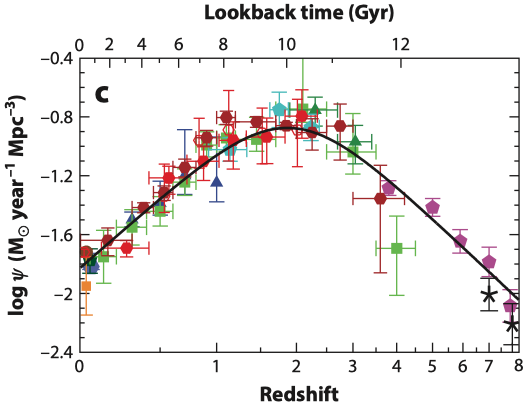
\includegraphics[width=.7\linewidth]{Chapter_1/Figures/Madau2014_Figure9.png}
    \caption[Reprint from \citet{Madau2014} (Figure~9)]{\label{fig:Madau2014_figure9}
        (Reprint from \citet{Madau2014}, Figure~9)\\
        This figure shows the cosmic star formation history from UV and IR emissions.
        For calculating SFR, they adopt Salpeter IMF\@.
        The black solid line shows the best fitting line.
        We can see the peak of SFR density in the universe at $z\sim1.9$
    }
\end{figure}

Although now we know the cosmic star formation history up to $z\sim8$ ($z > 4$ is still ambiguous due to the lack of IR observation), extending it to the earlier universe is quite difficult because we do not have a telescope to observe IR luminosity from high-z galaxies with a large field of view.
FUV emission from high-z galaxies is also difficult to be calibrated because the dust correction for high-z galaxies still have a large uncertainty.

On the contorary, the low-frequency emission is a extinction-free estimator and we will be able to observe high-z galaxies with a high sensitivity and large field of view enough to extend the cosmic star formation history.





\section{Low radio frequencies and SFR}\label{sec:lowradiofrequenciesandsfr}

The low-frequency radio emission from star-forming galaxies has been studied for many years.
In this paper, we use the term ``Low frequency'' as the frequency of a few $\mr{GHz}$ and less than that.
At this frequency range, synchrotron emission is supposed to be dominant in star-forming galaxies \citep{Condon1992a}.
The importance of this emission increased after the global log-linear correlation with infrared (IR) had been found.
This correlation was discovered by \citet{Helou1985} using integrated far-infrared (FIR;\@$60\,\micron$ and $100\,\micron$) and $1.4\GHz$ radio luminosities in star-forming galaxies (Figure~\ref{fig:Helou1985_figure2}).
Hereafter, we use the term ``IR-Radio Correlation (IRC)'' although this correlation is originally called FIR-Radio Correlation.
This is because we tend to examine the correlation of radio with the total IR luminosity instead of FIR after \citet{Bell2003}.

\begin{figure}[htbp]
	\centering
	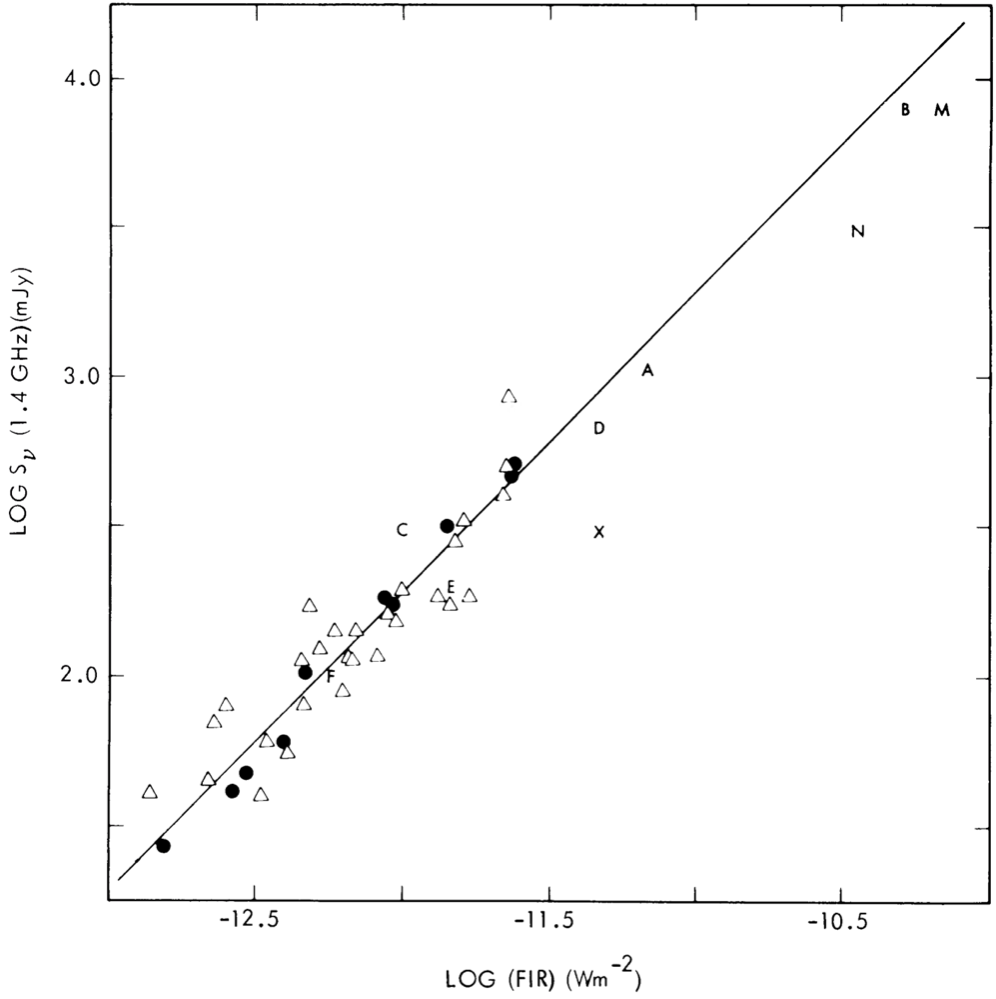
\includegraphics[width=.6\linewidth]{Chapter_1/Figures/Helou1985_Figure2.png}
    \caption[Adapted from \citet{Helou1985} (Figure~2)]{\label{fig:Helou1985_figure2}
        (Adapted from \citet{Helou1985}, Figure~2)\\
        This figure shows the comparison between FIR and radio at $1.4\GHz$ fluxes for each galaxy.
        We can see the tight correlation between them.
    }
\end{figure}

\citet{Condon1991a,Yun2001a, Bell2003} have examined this global correlation using a different sample set and found it holds the tightness across more than three orders of magnitude.
Recently, the low-frequency survey at around $100\MHz$ was operated by the LOw Frequency Array (LOFAR;~\citealt{VanHaarlem2013}) and the Murchison Widefield Array (MWA;~\citealt{Tingay2013a}).
With the advent of these telescopes, \citet{CalistroRivera2017a, Read2018, Wang2019} extend the study to at an order of magnitude lower frequency and find the correlation is held at not only $1.4\GHz$ but also $\sim 100\MHz$.
Thanks to this correlation, we can regard the low-frequency emission as a SFR indicator.
Synchrotron emission supposed to be dominant at low frequencies is emitted by the high-energy electrons accelerated by supernova remnants with the magnetic field in a galaxy, and it should trace the star formation activity in star-forming galaxies.
% Write a Calorimeter model
To explain IRC physically, \citet{Volk1989} proposed ``the calorimeter model''.
This model says that all energies from high energy electrons consumed before they escaping from galaxies is linearly correlated with all energies re-radiated as IR emissions by dust absorbing all FUV emission from young stars.
If this model is valid, IRC has a slope of unity.
However, recent studies shows that the slope is not unity and calorimeter model is not always accurate \citep{CalistroRivera2017a, Read2018}.
Since the low-frequency emission is not affected by the dust extinction \citep{Yun2001a, Murphy2011} and it will be observed from distant galaxies by the future extended survey, we anticipate its usefulness and need a further investigation of the relation between the radio and IR luminosities, especially its frequency dependence.

However, the spatially-resolved studies show that a star-forming galaxy emits the radio emission whose spectral index depends on the galaxy region \citep{Kapinska2017a, For2018a, Heesen2019} (Figure~\ref{fig:Kapinska2017_Figure5} and~\ref{fig:For2018_Figure6}).
This means that the radio emission is sensitive to the local density environment of the ISM and it is not guaranteed a simple frequency dependence of the global relation between the integrated radio and IR luminosities.

\begin{figure}[htbp]
	\centering
	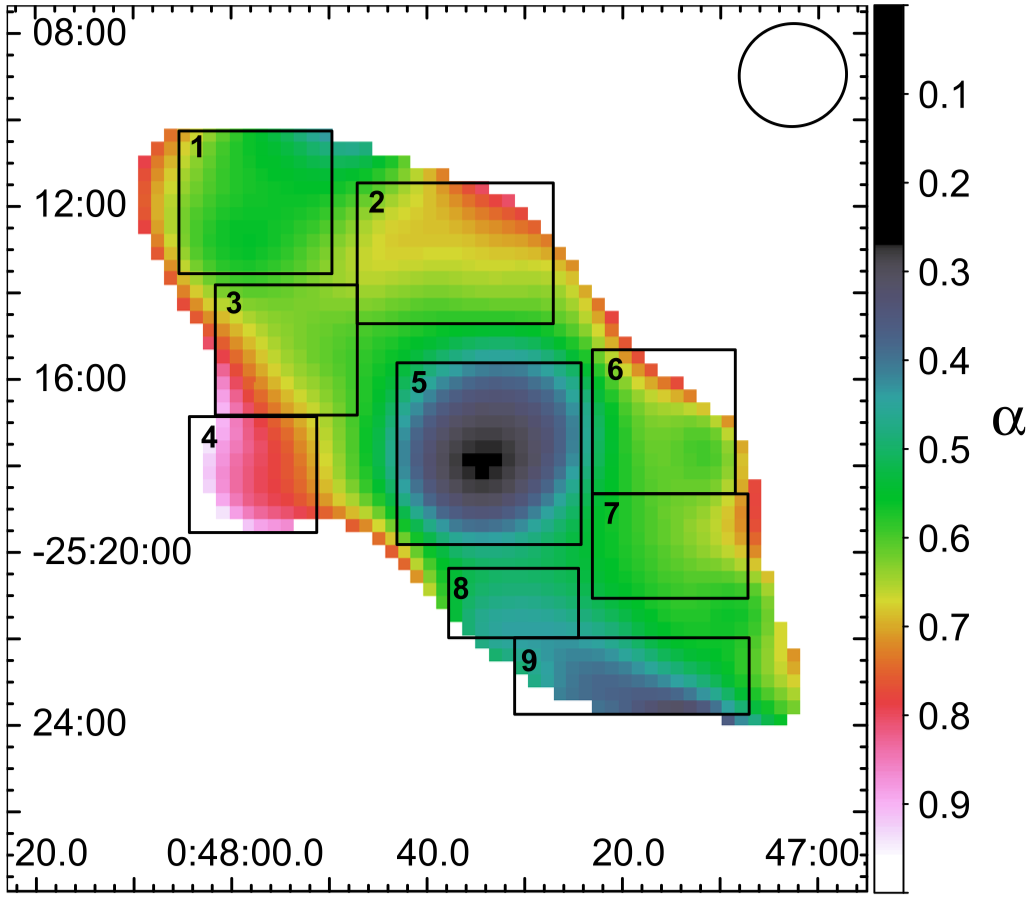
\includegraphics[width=.6\linewidth]{Chapter_1/Figures/Kapinska2017_Figure5.png}
    \caption[Adaptedfrom \citet{Kapinska2017a} (Figure~5)]{\label{fig:Kapinska2017_Figure5}
        (Adapted from \citet{Kapinska2017a}, Figure~5)\\
        This figure shows the distribution of the radio spectral index in NGC 253.
        They do the fitting between $200\MHz$ (GLEAM;\@\citealt{Hurley-Walker2017a}) and $1.465\GHz$ \citep{Carilli1992}.
        The color scale is for the spectral index and the pixel size is $18 \times 18 \arcs^2$.
    }
\end{figure}

\begin{figure}[htbp]
	\centering
	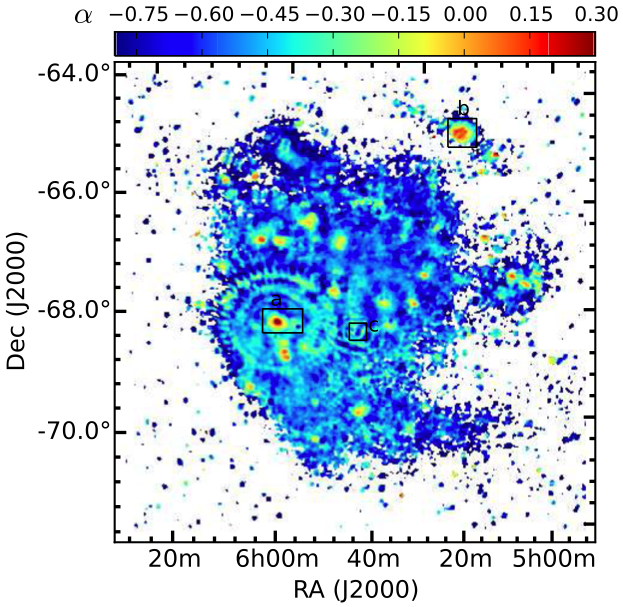
\includegraphics[width=.6\linewidth]{Chapter_1/Figures/For2018_Figure6.png}
    \caption[Adapted from \citet{For2018a} (Figure~6)]{\label{fig:For2018_Figure6}
        (Adapted from \citet{For2018a}, Figure~6)\\
        This figure shows the distribution of the radio spectral index in Large Magellanic Could (LMC).
        They do the fitting between $166\MHz$ (GLEAM;\@\citealt{Hurley-Walker2017a}) and $1.4\GHz$ \citep{Hughes2007}.
        The color scale is for the spectral index and the pixel size is $34.9 \times 34.9 \arcs^2$ at GLEAM 166MHz.
    }
\end{figure}

The integrated radio emission in star-forming galaxies across $100\MHz$ to $1.4\GHz$ is supposed to compose of a few percent to $10\%$ free-free and the synchrotron radiations \citep{Condon1992a}.
Each radiation is emitted by electrons interacted with the electric field of ions in the \ih~region or the magnetic field in a galaxy.
For emitting the synchrotron radiation, an electron needs to be accelerated to the light speed by the supernova remnant.
While the synchrotron emission is expected to be dominant at these low frequencies, previous studies find the sign of the free-free absorption and flatter or turnover spectral \citep{Schober2017, Chyzy2018}.
If the radio emission has a significant turnover among low frequencies, global IRC does not have a simple frequency dependence and the radio emission is no longer useful as a SFR indicator.

In this study, we investigate nearby star-forming galaxies from the reference sample for ensuring the reliability of measuring the SFR from the low-frequency emission.
For examining the general trend, we use star-forming galaxy samples from the Herschel Reference Survey (HRS;~\citealt{Boselli2010}) catalog which are supposed to represent the galaxy samples and the low-frequency emission from The GaLactic Extragalactic All-sky MWA (GLEAM;~\citealt{Hurley-Walker2017a}) survey which observes the mJy scale radio emission from large areas with their 20 narrow bands.

This paper is organized as follows.
In Chapter~\ref{chap:data}, I introduce our galaxy samples and the low-frequency emissions used in this study.
In Chapter~\ref{chap:methods}, I mention the way to investigate its frequency dependence and derive the radio SFR\@.
In Chapter~\ref{chap:results}, I show our results about the frequency dependence of IRC and the consistency of the radio SFR\@.
In Chapter~\ref{chap:discussions}, I compare our results with previous studies.
Finally, we summarize our study in Chapter~\ref{chap:summary}.



%\bibliographystyle{mnras}
%%\bibliography{example} % if your bibtex file is called example.bib
%\bibliography{masterthesis}




%Reference Table \ref{tab:Table1}.  And blah blah blah.
%
%\begin{table}[t]
%\caption[TOC Table Description]{Caption.}
%	\centering
%	\begin{tabular}{lcc}
%		\hline
%        {\textbf{Setting}}                      & \multicolumn{2}{c}{\textbf{Mt C/y}} \\
%		                                                           &         Min          &     Max      \\ \hline
%		AAA                         &          40          &      66      \\
%		BBB                               &          14          &      66      \\
%		CCC                                       &          18          &      43      \\
%		DDD      &          4           &    $>$12     \\
%		EEE                                  &          0           &      47      \\
%		FFF                    & 1$ \times $10$^{-4}$ &      52      \\
%		GGG &          8           &      42      \\ \hline
%	\end{tabular}
%    \label{tab:Table1}
%\end{table}
%
%\section{Figures}
%Reference Figure~\ref{fig:Fig1}.
%
%\subsection{This is a subsection}
%\begin{figure}[t]
%	\centering
%	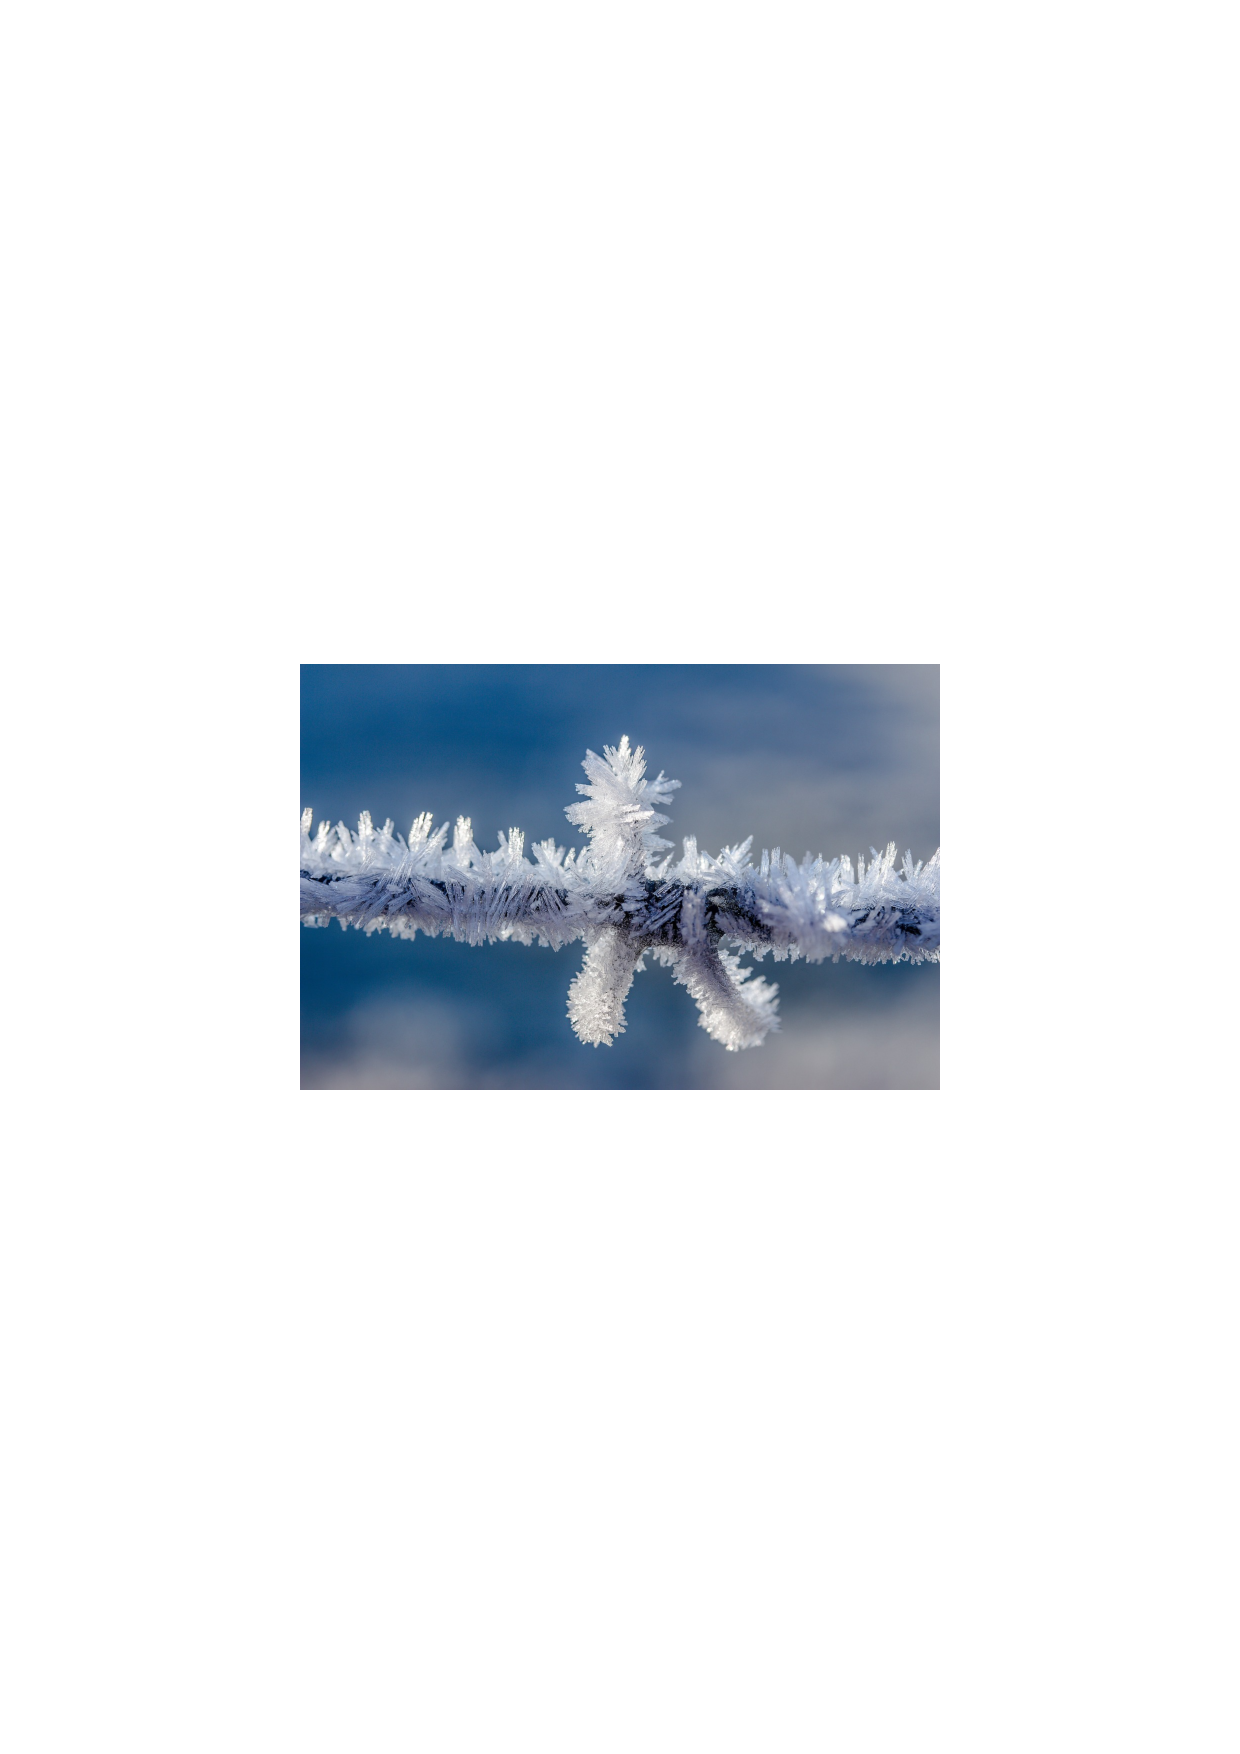
\includegraphics[width=.6\linewidth]{sFigs/Fig1.pdf}
%	\caption[TOC Figure Description]{Caption.}
%	\label{fig:Fig1}
%\end{figure}
%\subsubsection{This is a subsubsection}
%Citations are like \cite{goossens93,AbedonHymanThomas2003}.  Or maybe \cite{Abedon1994} said something.  Or \cite{Cerveny} which is an example of how to make a bib file that includes an author whose name begins with a non-English character and \cite{forgues96}: an example of referencing a Ph.D. thesis and yet more non-English characters.




%\bibliographystyle{abbrvnat}
%\bibliography{Chapter_1/ref1}

    \chapter{Theoretical Background}\label{chap:theory}
\begin{chapabstract}

    In this chapter, I describe physical mechanisms of radio emissions related to our study.
    At low frequencies, we observe free-free\footnote{\url{https://www.cv.nrao.edu/~sransom/web/Ch4.html}} (Bremsstrahlung) and synchrotron\footnote{\url{https://www.cv.nrao.edu/~sransom/web/Ch5.html}} radiations.
    Both radiations are the continuum emission.
    While the free-free radiation is usually dominant from a galaxy at $30 \sim 200\GHz$, the synchrotron radiation is dominant less than $30\GHz$ (Figure~\ref{fig:Condon1992_figure1}).\\ \vspace{0.2cm}
\begin{figure}[htbp]
	\centering
	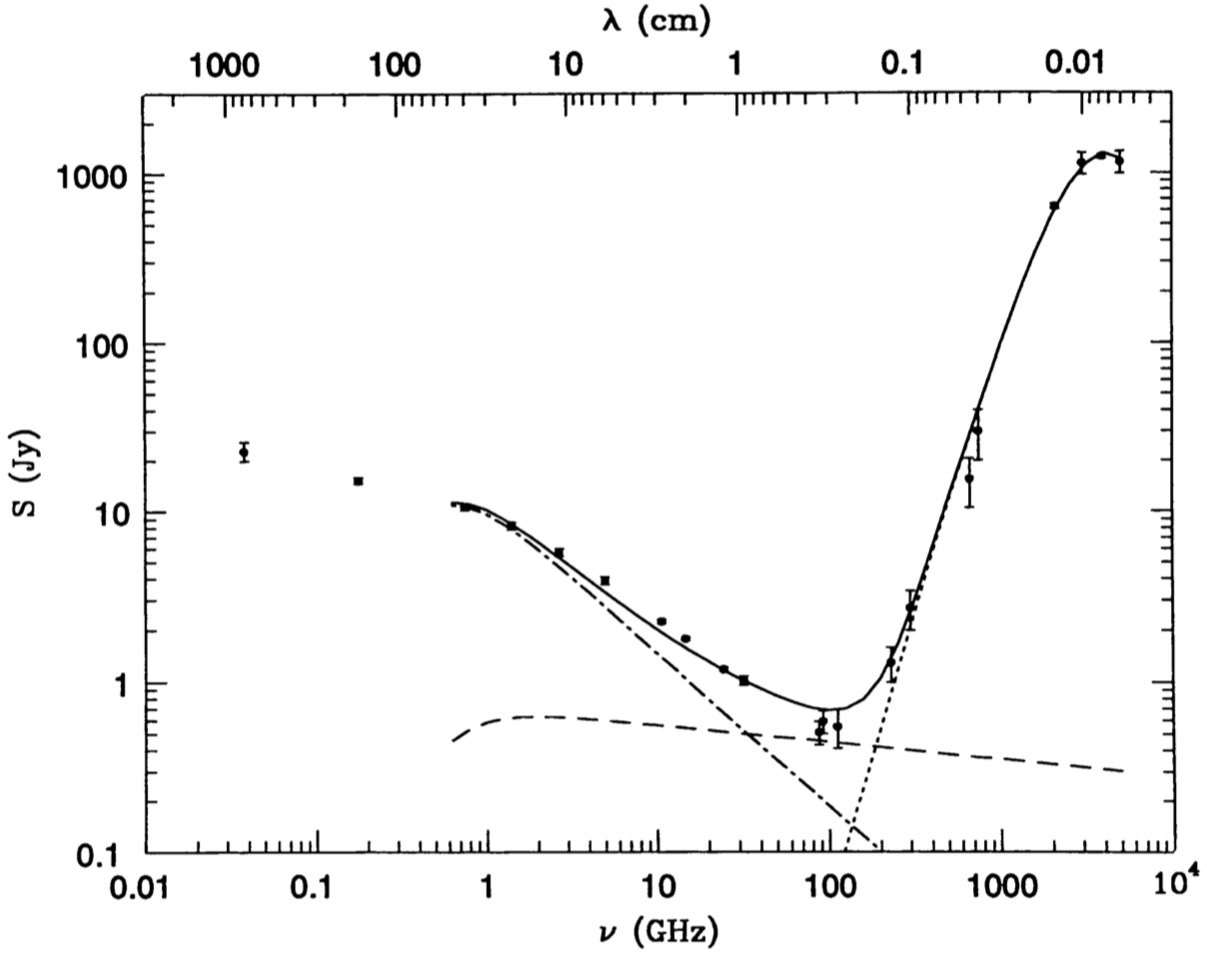
\includegraphics[width=.7\linewidth]{Chapter_2/Figures/Condon1992_Figure1.png}
    \caption[Reprint from \citet{Condon1992a} (Figure~1)]{\label{fig:Condon1992_figure1}
        (Reprint from \citet{Condon1992a}, Figure~1)\\
        This figure shows the spectral energy distribution of M82.
        The dotted line shows the dust thermal emission which is dominant at higher than $200\GHz$.
        The dashed line shows the free-free radiation from the \ih~regions around massive stars, which is dominant at $30 \sim 200\GHz$.
        The dot-dash line shows the synchrotron radiation emitted by the high energy electrons, which is dominant at less than $30\GHz$.
    }
\end{figure}

\end{chapabstract}



\section{Free-free radiation}\label{sec:freefreeradiation}

The free electrons produce free-free radiation by scattering off ions.
In star-forming galaxies, the radiation source is the \ih~region where young massive (OB) stars ionized most of the hydrogen atoms.
In this section, we consider the radiation mechanism of free-free radiation.
Here, I consider only electrons emit the radiation because an electron is much more accelerated than an ion due to the difference of their mass (an electron is 1840 times lighter than a proton).

Firstly, I consider the simplest case that a single electron passes by the ion and emits the radiation.
Note that the path of the electron does not change after the interaction because the energy of radio emission is much smaller than the mean electron energy in a plasma:

\begin{equation}\label{eq:essential_radio4n12}
    \frac{E\msb{10\GHz}}{\bra{E_e}} = \frac{h \times 10^{10}\,\mr{Hz}}{3kT / 2} = \frac{6.63 \times 10^{-27} \mr{erg\,s} \times 10^{10}\,\mr{Hz}}{1.5 \cdot 1.38 \times 10^{-16}\,\mr{erg\,K^{-1}} \cdot 10^4\,\mr{K}} = 3.3 \times 10^{-5}
\end{equation}

During the interaction, the electron is accelerated by the electric field by the ion.
Then, we can write the equation of motion for parallel and perpendicular to the electron's path (Figure~\ref{fig:nrao_radio4n2}):

\begin{figure}[htbp]
	\centering
	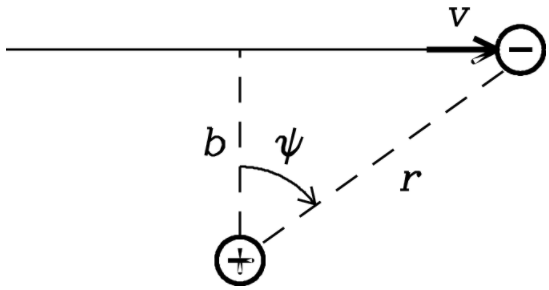
\includegraphics[width=.5\linewidth]{Chapter_2/Figures/NRAO_radio4n2.png}
    \caption[The schematic image of the interaction of an electron with the ion]{\label{fig:nrao_radio4n2}
        This figure shows the schematic picture of the interaction of an electron with the ion.
        $b$ and $\tau = b/v$ are called the impact parameter and the collision time, respectively.
    }
\end{figure}
\begin{align}
    F_{\|} &= m_{\mr{e}} \dot{v}_{\|}=\frac{-Z e^{2}}{r^{2}} \sin \psi=\frac{-Z e^{2} \sin \psi \cos ^{2} \psi}{b^{2}}\label{eq:essential_radio4n15}\\
    F_{\perp} &= m_{\mr{e}} \dot{v}_{\perp}=\frac{Z e^{2}}{r^{2}} \cos \psi=\frac{Z e^{2} \cos ^{3} \psi}{b^{2}}\label{eq:essential_radio4n16}
\end{align}
where $b$ is the impact parameter and $\cos\psi = \frac{b}{r}$.

These accelerations show different shapes of the pulse (Figure~\ref{fig:nrao_radio4n3}).
Since the parallel acceleration produces some infrared radiation with the angular frequency $\omega \sim \tau^{-1} = \frac{v}{b}$ ($\tau$ is the collision time), its contribution is negligible at radio frequency.

\begin{figure}[htbp]
\centering
	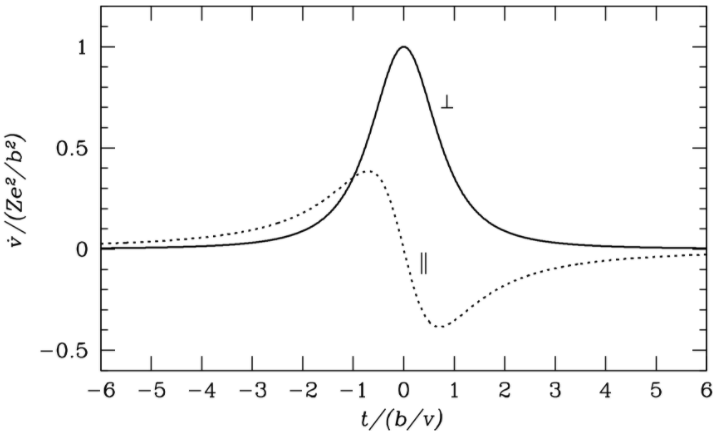
\includegraphics[width=.7\linewidth]{Chapter_2/Figures/NRAO_radio4n3.png}
    \caption[The acceleration of an electron by an ion]{\label{fig:nrao_radio4n3}
        This figure shows the acceleration of an electron.
        The solid and dotted lines show the case of perpendicular and parallel to the electron's velocity, respectively.
    }
\end{figure}

Therefore, the power of free-free radiation from the acceleration perpendicular to the electron's velocity is:

\begin{equation}\label{eq:essential_radio4n17}
    P=\frac{2}{3} \frac{e^{2} \dot{v}_{\perp}^{2}}{c^{3}}=\frac{2 e^{2}}{3 c^{3}} \frac{Z^{2} e^{4}}{m_{\mr{e}}^{2}}\brp{\frac{\cos ^{3} \psi}{b^{2}}}^{2}
\end{equation}
where we insert $\dot{v}_{\perp}$ into the Larmor's formula $\brp{P = \frac{2}{3}\frac{q^2\dot{v}^2}{c^3},\,q\,\mr{is\,a\,charge}}$, which shows the power emitted by the accelerated particles.

We can get the total energy of $W$ by the pulse as follows:

\begin{equation}\label{eq:essential_radio4n18}
    W = \int^{\infty}_{-\infty} P\,\mr{d}t
\end{equation}

As I have noted above, the electron's velocity does not change so that we can change of variables:

\begin{equation}\label{eq:essential_radio4n19}
    v = \frac{\rd x}{\rd t}\ \ \ \mr{and}\ \ \ \tan\psi = \frac{x}{b}
\end{equation}

then,

\begin{equation}\label{eq:essential_radio4n20}
    v=\frac{b\,\rd\brp{\tan \psi}}{\rd t} = \frac{b\,\rd \psi}{\cos ^{2}\psi\,\rd t}
\end{equation}

and

\begin{equation}\label{eq:essential_radio4n21}
    \rd t=\frac{b}{v} \frac{\rd \psi}{\cos ^{2} \psi}
\end{equation}

Substituting Equation~\ref{eq:essential_radio4n17} and~\ref{eq:essential_radio4n21} into Equation~\ref{eq:essential_radio4n18} yields

\begin{equation}\label{eq:essential_radio4n22}
    W=\frac{2}{3} \frac{Z^{2} e^{6}}{c^{3} m_{\mathrm{e}}^{2} b^{4}} \int_{-\pi / 2}^{\pi / 2} \frac{b}{v} \frac{\cos ^{6} \psi}{\cos ^{2} \psi} \rd \psi=\frac{4}{3} \frac{Z^{2} e^{6}}{c^{3} m_{\mathrm{e}}^{2} b^{3} v} \int_{0}^{\pi / 2} \cos ^{4} \psi\ \rd \psi = \frac{\pi Z^2 e^6}{4 c^3 m_{\mr{e}}^2}\brp{\frac{1}{b^3v}}
\end{equation}
where $\int_{0}^{\pi / 2} \cos ^{4} \psi\,\rd \psi=\frac{3 \pi}{16}$.

The pulse energy $W$ shows the total energy emitted by a single electron interaction characterized by the impact parameter $b$ and the electron's velocity $v$.\\ \vspace{0.2cm}

Secondly, I consider the strength and spectral of free-free radiation from \ih~region with several simple assumptions.
Here, I assume the local thermodynamic equilibrium (LTE) in the \ih~region.
In LTE, electrons have a much higher speed than ions because of the difference of their mass, although the average kinetic energy of electrons and ions are equal.
Therefore, it is reasonable to think ions do not move by the interactions.

When I consider the cylindrical shell around the ion (Figure~\ref{fig:nrao_radio4n5}), I can calculate the number of electrons passing the ion per unit time between $b$ and $b + \rd b$ under the velocity range of $\rd v$:

\begin{figure}[htbp]
	\centering
	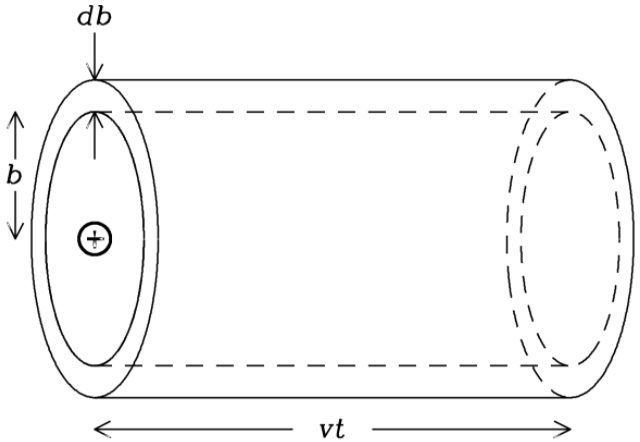
\includegraphics[width=.6\linewidth]{Chapter_2/Figures/NRAO_radio4n5.png}
    \caption[The schematic picuture of the cylindrical shell of electrons]{\label{fig:nrao_radio4n5}
        This figure shows the schematic picture that an electron passes the ion in the cylindrical shell.
    }
\end{figure}

\begin{equation}\label{eq:essential_radio4n27}
    n\msb{e} \brp{2\pi b,\rd b}\,v f\brp{v}\,\rd v
\end{equation}
where $f\brp{v}$ is the normalized speed distribution of electrons (In LTE, $f\brp{v}$ is the Maxwellian distribution).

The number $\dot{n}\msb{c}\brp{v,\,b}$ of such collisions per unit volume per unit time is:

\begin{equation}\label{eq:essential_radio4n28}
    \dot{n}\msb{c}\brp{v,\,b} = \brp{2\pi b} v f\brp{v} n\msb{e} n\msb{i}
\end{equation}

Then, I can write the emission coefficient $j_{\nu}$ as follows:

\begin{equation}\label{eq:essential_radio4n29}
    4 \pi j_{\nu}=\int_{b=0}^{\infty} \int_{v=0}^{\infty} W_{\nu}\brp{v,\,b} \dot{n}\msb{c}\brp{v,\,b} \rd v \rd b
\end{equation}
where $W\msb{\nu}\brp{v,\,b}$ is the average energy per unit frequency emitted during a single interaction and approximately written in $W\msb{\nu}\brp{v,\,b} = \frac{W}{\nu\msb{\max} \brp{= v/2\pi b}}$.

Substituting $W\msb{\nu}\brp{v,\,b}$ and Equation~\ref{eq:essential_radio4n28} into Equation~\ref{eq:essential_radio4n29} yields

\begin{align}
    4 \pi j_{\nu} &= \int_{b=0}^{\infty} \int_{v=0}^{\infty} \brp{\frac{\pi^2 Z^2 e^6}{2 c^3 m\msb{e}^2 b^2 v^2}} 2 \pi b\,\rd b\,n\msb{e} n\msb{i}\,v\,f(v) \rd v \label{eq:essential_radio4n30}\\
                  &=\frac{\pi^{3} Z^{2} e^{6} n\msb{e} n\msb{i}}{c^{3} m\msb{e}^{2}} \brp{\frac{2m\msb{e}}{\pi k T}}^{1/2}\int_{b=0}^{\infty} \frac{\rd b}{b}\label{eq:essential_radio4n31}
\end{align}
where I use the Maxwellian distribution:

\begin{equation}\label{eq:essential_radio4n34}
    f(v)=\frac{4 v^2}{\sqrt{\pi}} \brp{\frac{m\msb{e}}{2 k T}}^{3/2} \exp \brp{-\frac{m\msb{e} v^2}{2 k T}}
\end{equation}

Note that $\int^{\infty}_{b=0} \frac{\rd b}{b}$ diverges, so it needs finite limites $b_{\min}$ and $b_{\max}$.
To estimate $v_{\min}$, let's consider the change in momentum during the single electron-ion interaction:

\begin{align}\label{eq:essential_radio4n40}
    m\msb{e} \Delta v &= \int_{-\infty}^{\infty} F \rd t = \int_{-\infty}^{\infty}\left(\frac{Z e^{2} \cos \psi}{r^{2}}\right) \rd t=Z e^{2} \int_{-\infty}^{\infty} \frac{\cos ^{3} \psi}{b^{2}} \rd t \\
                      &= \frac{Z e^{2}}{b v} \int_{-\pi / 2}^{\pi / 2} \cos \psi\,\rd \psi=\frac{2 Z e^{2}}{b v} \\
                      &= \frac{2Ze^2}{bv} \brp{< 2m\msb{e}v}
\end{align}
where the maximum momentum transfer $m\msb{e} \Delta v$ is twice the initial momentum $m\msb{v}$. \\

Therefore, the minimum impact parameter $b_{\min}$ is

\begin{equation}\label{eq:essential_radio4n43}
    b_{\min} = \frac{Ze^2}{m\msb{e}v^2}
\end{equation}

To estimate the maximum impact parameter $b_{\max}$, let's consider $\nu_{\max}$ and get $b_{\max} = \frac{v}{2\pi \nu}$ because the pulse power is not significant at frequency $\nu$ above $\nu_{\max}$.
In some textbooks, they consider $b_{\max}$ with the Debye length, which shows the characteristic scale of the electric shielding.
However, this length scale is much larger than $b_{\max}$ obtained here, and it is inappropriate for the calculation in the typical \ih~region.

These limits ($b_{\min}$, $b_{\max}$) yield

\begin{equation}\label{eq:essential_radio4n49}
    \frac{b_{\max }}{b_{\min }} \sim \brp{\frac{3 k T}{m\msb{e}}}^{1 / 2}\brp{2 \pi \nu}^{-1}\brp{\frac{3 k T}{Z e^{2}}} \sim \brp{\frac{3 k T}{m\msb{e}}}^{3 / 2} \frac{m\msb{e}}{2 \pi Z e^{2} \nu} \sim 10^5
\end{equation}

However, this value varies logarithmically in Equation~\ref{eq:essential_radio4n51}.
Therefore, these limits have little effect on the calculation.

Since the \ih~region is in LTE, it is possible to consider Kirchhoff's low and absorption coefficient $\kappa$ in the Rayleigh-Jeans limit:

\begin{equation}\label{eq:essential_radio4n51}
    \kappa=\frac{j_{\nu}}{B_{\nu}(T)} \sim \frac{j_{\nu} c^2}{2 k T \nu^2} = \frac{1}{\nu^2 T^{3/2}}\brb{\frac{Z^2 e^6}{c} n\msb{e} n\msb{i} \frac{1}{\sqrt{2\pi\brp{m\msb{e} k}^3}}} \frac{\pi^2}{4} \ln \brp{\frac{b_{\max}}{b_{\min}}}
\end{equation}
where $B_{\nu}\brp{T}$ is the blackbody brightness.

The absorption coefficient $\kappa$ is proportional to $\nu^{-2}$ (To be precise, it is proportional to $\nu^{-2.1}$ due to the frequency dependence of $b_{\max}$).

Now I can calculate the total opacity $\tau$ of \ih~region if I assume the simple cylindrical shape with a uniform density for the \ih~region (Figure~\ref{fig:nrao_radio4n7}):

\begin{figure}[htbp]
	\centering
	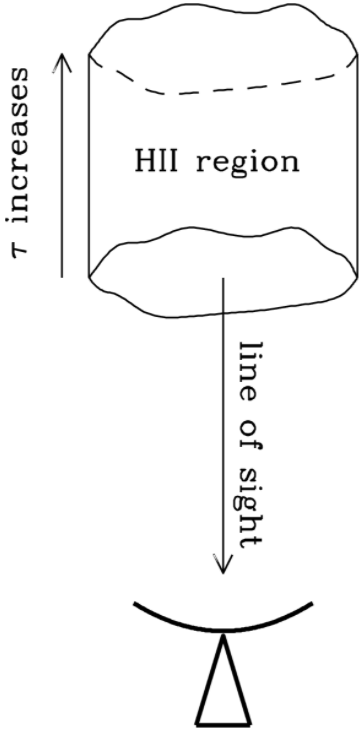
\includegraphics[width=.3\linewidth]{Chapter_2/Figures/NRAO_radio4n7.png}
    \caption[The schematic picture of \ih~region]{\label{fig:nrao_radio4n7}
        This figure shows the schematic picture of the \ih~region.
        Astronomers often approximate \ih~regions by the uniform cylinders.
        Cylindrical assumption lets us to calculate optical depth $\tau$ easily.
    }
\end{figure}

\begin{equation}\label{eq:essential_radio4n53}
\tau=-\int\msb{los} \kappa\,\rd s \propto \int \frac{n\msb{e} n\msb{i}}{\nu^{2.1} T^{3/2}} \rd s \sim \int \frac{n\msb{e}^2}{\nu^{2.1} T^{3/2}} \rd s
\end{equation}
where $s$ is the depth of \ih~region parallel to the line of sight.

At low frequencies enough that $\tau \gg 1$, the \ih~region becomes opaque, and the spectrum approaches the blackbody.
In this case, the brightness temperature approaches the electron temperature $\brp{T\sim10^4\,\mr{K}}$ and its flux density $S$ is in the Rayleigh-Jeans limit $\brp{S \propto \nu^2}$.
On the other hand, at frequency $\tau \ll 1$, the \ih~region is transparent and $S \propto \frac{2kT\nu^2}{c^2}\tau\brp{\nu} \propto \nu^{-0.1}$.

I show the spectrum of free-free radiation in the \ih~region in Figure~\ref{fig:nrao_radio4n8}.

\begin{figure}[htbp]
	\centering
	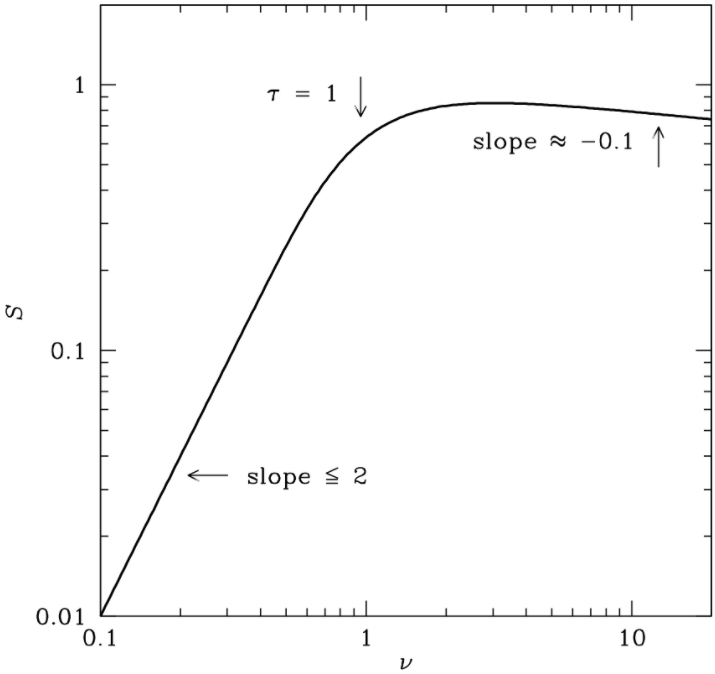
\includegraphics[width=.7\linewidth]{Chapter_2/Figures/NRAO_radio4n8.png}
    \caption[The spectrum of free-free radiation]{\label{fig:nrao_radio4n8}
        This figure shows the radio spectrum of free-free radiation.
        At low frequencies, we can see the blackbody with the slope $\leq 2$.
        The assumption of the uniform cylinder gives the slope $~2$, but the nonuniform \ih~region emits free-free radiation with the slope less than 2.
        At frequencies higher than the frequency of $\tau=1$, the slope is nearly flat $\brp{-0.1}$.
    }
\end{figure}

At low frequencies, the spectral index $\alpha$ on the log-log plot is useful to describe the density condition.
The definition of $\alpha$ is below:

\begin{equation}\label{eq:essential_radio4n55}
    \alpha \equiv \pm \frac{\rd \log S}{\rd \log \nu}
\end{equation}
where the sign depends on the literature.

With the $+$ sign convention, the spectral index of \ih~region well above the break frequency $\brp{\tau=1}$ is $\alpha=-0.1$.\\ \vspace{0.2cm}

Finally, I mention the idea of emission measure (EM) often used for understanding the physical condition in the \ih~region.
The definition of EM is

\begin{equation}\label{eq:essential_radio4n57}
    \frac{\mr{EM}}{\mr{pc} \cdot \mr{cm}^{-6}} \equiv \int\msb{los}\brp{\frac{n\msb{e}}{\mr{cm}^{-3}}}^2 \rd\brp{\frac{s}{\mr{pc}}}
\end{equation}

Then, we can write the optical depth $\tau$ in

\begin{equation}\label{eq:essential_radio4n58}
    \tau \sim 3.014 \times 10^{-2}\brp{\frac{T}{\mr{K}}}^{-3/2}\brp{\frac{\nu}{\mr{GHz}}}^{-2}\brp{\frac{\mr{EM}}{\mr{pc} \cdot \mr{cm}^{-6}}}\bra{g\msb{ff}}
\end{equation}
where $\bra{g\msb{ff}}$ is the free-free Gaunt factor:

\begin{equation}\label{eq:essential_radio4n59}
    \bra{g\msb{ff}} \sim \ln \brb{4.955 \times 10^{-2}\brp{\frac{\nu}{\mr{GHz}}}^{-1}}+1.5 \ln \brp{\frac{T}{\mr{K}}}
\end{equation}

\citet{Mezger1967} found the excellent approximation for the free-free opacity $\tau$ is

\begin{equation}\label{eq:essential_radio4n60}
    \tau \sim 3.28 \times 10^{-7}\brp{\frac{T}{10^4 \mr{K}}}^{-1.35}\brp{\frac{\nu}{\mr{GHz}}}^{-2.1}\brp{\frac{\mr{EM}}{\mr{pc} \cdot \mr{cm}^{-6}}}
\end{equation}

When we observe the break frequency $\nu$ $\brp{\tau \sim 1}$, then we can calculate EM with the electron temperature $\brp{\sim10^4\,\mr{K}}$.
And also, we can calculate the gas density in the \ih~region if we know its size (depth).





\section{Synchrotron radiation}\label{sec:synchrotronradiation}

Synchrotron radiation is a continuum emission which is usually dominant at less than $30\GHz$ in star-forming galaxies.
The interaction of high energy (relativistic) electrons accelerated by the supernova remnant or the galactic nuclei with the galactic magnetic field causes the radiation.
Since high energy electrons have a power-law energy distribution (not Maxwellian), we usually call the radiation ``non-thermal synchrotron radiation''.
If electrons have a much smaller velocity than the light, they emit the cyclotron radiation with the cyclotron frequency $\omega = \frac{eB}{m\msb{e}c}$ in cgs unit ($e$ is a charge, $B$ is the strength of the magnetic field, $m\msb{e}$ is a mass of an electron and $c$ is the speed of light).
In the normal star-forming galaxies ($B\sim10\mu G$), the electron gyro frequency is $30\,\mr{Hz}$ and we cannot observe it because it is much smaller frequency than the plasma frequency.

In this section, I show the mechanism to emit synchrotron radiation.
Firstly, I focus on synchrotron radiation emitted by a single electron.
Here, I use primed coordinates for the inertial frame in which an electron is at rest and unprimed coordinates for the frame of an observer at rest.
Then, I can write down the radiated power with Larmor's equation in the electron rest frame:

%Equation(5.24)
\begin{equation}\label{eq:essential_radio5n24}
    P^{\prime}=\frac{2\brp{e^{\prime}}^{2}\brp{a_{\perp}^{\prime}}^{2}}{3 c^{3}}=\frac{2 e^{2}\brp{a_{\perp}^{\prime}}^{2}}{3 c^{3}}
\end{equation}
where $e'=e$ because the electric charge is a relativistic invariant.

If an electron passes on $x$-axis in the magnetic field, its acceleration is only $y$ and $z$-axis because of the definition of Lorentz force.
Applying the chain rule to the acceleration by the magnetic field $a_{\perp} = \brp{a^2_y + a^2_z}^{1/2}$ in the rest frame of an observer yields

%Equation(5.25)
\begin{equation}\label{eq:essential_radio5n25}
    a_y \equiv \frac{\rd v_y}{\rd t}=\frac{\rd v_y}{\rd t^{\prime}} \frac{\rd t^{\prime}}{\rd t}=\frac{1}{\gamma} \frac{\rd v_y^{\prime}}{\rd t^{\prime}} \frac{\rd t^{\prime}}{\rd t}=\frac{a_y^{\prime}}{\gamma^2}\ \ \ \brp{a_z \equiv \frac{\rd v_z}{\rd t} = \frac{a'_z}{\gamma^2}}
\end{equation}

Then,

%Equation(5.26)
\begin{equation}\label{eq:essential_radio5n26}
    a_{\perp}=\frac{a_{\perp}^{\prime}}{\gamma^{2}}
\end{equation}

Thus,

%Equation(5.27)
\begin{equation}\label{eq:essential_radio5n27}
    P^{\prime}=\frac{2 e^{2}\brp{a_{\perp}^{\prime}}^{2}}{3 c^{3}}=\frac{2 e^{2} a_{\perp}^{2} \gamma^{4}}{3 c^{3}}
\end{equation}

Now, I need to transform $P' = \frac{\rd E'}{\rd t'}$ into $P = \frac{\rd E}{\rd t}$.
The chain rule derives

%Equation(5.28)
\begin{equation}\label{eq:essential_radio5n28}
    P \equiv \frac{\rd E}{\rd t}=\frac{\rd E}{\rd t^{\prime}} \frac{\rd t^{\prime}}{\rd t}=\frac{\rd E}{\rd E^{\prime}} \frac{\rd E^{\prime}}{\rd t^{\prime}} \frac{\rd t^{\prime}}{\rd t}=\gamma P^{\prime} \gamma^{-1}=P^{\prime}
\end{equation}
where the radiated power is also the relativistic invariant.

Consequently,

%Equation(5.29)
\begin{equation}\label{eq:essential_radio5n29}
    P=P^{\prime}=\frac{2 e^{2} a_{\perp}^{2} \gamma^{4}}{3 c^{3}} \quad\left(a_{\|}=0\right)
\end{equation}

To calculate $a_{\perp}$, $a_{\perp} = \frac{\rd v_{\perp}}{\rd t} = \omega_B v_{\perp}$.
Since electrons emitting synchrotron radiation are relativistic, the angular frequency $\omega_{B}$ is $\omega_B = \frac{eB}{\brp{\gamma m\msb{e}}c}$.
Then,

%Equation(5.31)
\begin{equation}\label{eq:essential_radio5n31}
    a_{\perp}=\frac{e B v_{\perp}}{\gamma m_{\mathrm{e}} c}=\frac{e B v \sin \alpha}{\gamma m_{\mathrm{e}} c}
\end{equation}
where $\alpha$ shows the pitch angle between the electron velocity and the magnetic field $B$.

Inserting Equation~\ref{eq:essential_radio5n31} into Equation~\ref{eq:essential_radio5n29} yields

%Equation(5.32)
\begin{equation}\label{eq:essential_radio5n32}
    P=\frac{2 e^{2}}{3 c^{3}} \gamma^{2} \frac{e^{2} B^{2}}{m_{\mathrm{e}}^{2} c^{2}} v^{2} \sin ^{2} \alpha
\end{equation}

For simplicity, this equation often is written in

%Equation(5.37)
\begin{equation}\label{eq:essential_radio5n37}
    P=2 \sigma_{\mathrm{T}} \beta^{2} \gamma^{2} c U_{B} \sin ^{2} \alpha
\end{equation}
where $\sigma\msb{T}$ is the Thomson cross-section of an electron, $\beta=\frac{v}{c}$ and $U_B$ is the magnetic energy density $\brp{U_B = \frac{B^2}{8\pi}}$.

Therefore, the synchrotron power radiated by a single electron depends on $\gamma$, $U_B$ and $\alpha$ ($\beta\sim1$ if $\gamma \gg 1$)

The relativistic electrons can have lifetimes of thousands to millions of years before losing their energy via synchrotron radiation or other physical processes.
During their lifetimes, electrons scatter with the galactic magnetic field and charged particles repeatedly.

In this case, the distribution of the pitch angle $\alpha$ becomes random and isotropic, and we can derive the averaged synchrotron power $\bra{P}$ per electron over all possible $\alpha$:

%Equation(5.38)
\begin{equation}\label{eq:essential_radio5n38}
    \bra{P} = 2 \sigma\msb{T} \beta^2 \gamma^2 c U_B\bra{\sin^2 \alpha} = \frac{4}{3}\sigma\msb{T} \beta^2 \gamma^2 c U_B
\end{equation}
where
%Equation(5.39-41)
\begin{equation}\label{eq:essential_radio5n39}
    \begin{aligned}
    \bra{\sin^2 \alpha} & \equiv \frac{\int \sin^2 \alpha \rd \Omega}{\int \rd \Omega}=\frac{1}{4\pi} \int \sin^2 \alpha \rd \Omega \\
                        &=\frac{1}{4\pi} \int {\phi=0}^{2\pi} \int_{\alpha=0}^{\pi} \sin^2 \alpha \sin \alpha \rd \alpha \rd \phi=\frac{1}{4\pi} 2 \pi \frac{4}{3} \\
                        &=\frac{2}{3}
    \end{aligned}
\end{equation}

Here I describe the beaming effect, which is the specific feature of synchrotron radiation due to the relativistic electrons.
The relation between $v_x$ at the frame of the observer (unprimed) and $v'_x$  at the rest frame of the electron (primed) is

%Equation(5.43-45)
\begin{equation}\label{eq:essential_radio5n43}
    \begin{aligned}
        v_x \equiv \frac{\rd x}{\rd t} &= \frac{\rd x}{\rd t^{\prime}} \frac{\rd t^{\prime}}{\rd t}=\gamma\brp{\frac{\rd x^{\prime}}{\rd t^{\prime}}+v \frac{\rd t^{\prime}}{\rd t^{\prime}}}\brp{\frac{\rd t}{\rd t^{\prime}}}^{-1} \\
                                       &=\gamma\brp{v_x^{\prime}+v}\brb{\gamma\brp{1+\frac{\beta}{c} \frac{\rd x^{\prime}}{\rd t^{\prime}}}}^{-1} \\
                                       &=\brp{v_x^{\prime}+v}\brp{1+\frac{\beta v_x^{\prime}}{c}}^{-1}
    \end{aligned}
\end{equation}

In the $y$-direction,

%Equation(5.46-47)
\begin{equation}\label{eq:essential_radio5n46}
    \begin{aligned}
        v_y \equiv \frac{\rd y}{\rd t} &= \frac{\rd y}{\rd t^{\prime}} \frac{\rd t^{\prime}}{\rd t}=\frac{\rd y^{\prime}}{\rd t^{\prime}}\brp{\frac{\rd t}{\rd t^{\prime}}}^{-1} \\
                                       &= \frac{v_y^{\prime}}{\gamma}\brp{1+\frac{\beta v_x^{\prime}}{c}}^{-1}
    \end{aligned}
\end{equation}

In the electron's rest frame, if an electron emits synchrotron photons with speed $c$ at an angle $\theta'$ from $x'$-axis, then the relation among $\theta'$, $v'$ and $c$ is

%Equation(5.48)
\begin{equation}\label{eq:essential_radio5n48}
    \cos \theta^{\prime}=\frac{v_x^{\prime}}{c}, \quad \sin \theta^{\prime}=\frac{v_y^{\prime}}{c}
\end{equation}

In the observer's rest frame, we can write in the same way:

%Equation(5.49)
\begin{equation}\label{eq:essential_radio5n49}
    \cos \theta=\frac{v_x}{c}, \quad \sin \theta=\frac{v_y}{c}
\end{equation}

Using Equation~\ref{eq:essential_radio5n43},~\ref{eq:essential_radio5n46},~\ref{eq:essential_radio5n48} and~\ref{eq:essential_radio5n49} to eliminate $v$ and $v'$ yields the relation between $\theta$ and $\theta'$:

%Equation(5.50 and 51)
\begin{equation}\label{eq:essential_radio5n50}
    \begin{aligned}
        \cos \theta &= \brp{\frac{v_x^{\prime}+v}{1+\beta v_x^{\prime} / c}} \frac{1}{c}=\brp{\frac{c \cos \theta^{\prime}+v}{1+\beta c \cos \theta^{\prime} / c}} \frac{1}{c}=\frac{\cos \theta^{\prime}+\beta}{1+\beta \cos \theta^{\prime}} \\
        \sin \theta &= \frac{v_y^{\prime}}{c \gamma\brp{1+\beta v_{x}^{\prime} / c}} = \frac{\sin \theta^{\prime}}{\gamma\brp{1+\beta \cos \theta^{\prime}}}
    \end{aligned}
\end{equation}

In the electron's rest frame, Larmor's equation implies a power pattern proportional to $\cos^2\theta'$ with nulls at $\theta'=\pm \frac{\pi}{2}$.

In the observer's rest frame, in this case:

%Equation(5.52)
\begin{equation}\label{eq:essential_radio5n52}
    \sin\theta = \frac{1}{\gamma} \quad \rightarrow \quad \theta=\pm \arcsin (1 / \gamma)
\end{equation}

Therefore, observers see synchrotron radiation from the electron in a narrow beam angle $\brp{\frac{2}{\gamma}}$ and this effect is called ``Beaming effect'' (Figure~\ref{fig:nrao_radio5n3})

%Figure(5.3)
\begin{figure}[htbp]
	\centering
	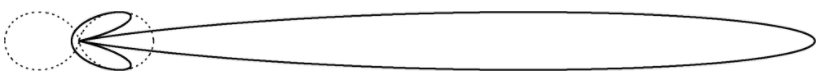
\includegraphics[width=.7\linewidth]{Chapter_2/Figures/NRAO_radio5n3.png}
    \caption[The schematic picture of relativistic aberration]{\label{fig:nrao_radio5n3}
        This figure shows the beaming effect which is a narrow angle for the radiation towards the observer.
        The dotted curve shows the original dipole power pattern of Larmor radiation and the solid line shows the case of $\gamma = 5$.
    }
\end{figure}

The beaming effect allows observers to see a short pulse of the radiation.
Note that the duration $\Delta t\msb{p}$ for observing the pulse is shorter than the time $\Delta t$, which the electron passes the narrow region $\brp{\frac{2}{\gamma}}$ because the electron moves toward the observer with the speed $\sim c$ (Figure~\ref{fig:nrao_radio5n4}).

%Figure(5.4)
\begin{figure}[htbp]
	\centering
	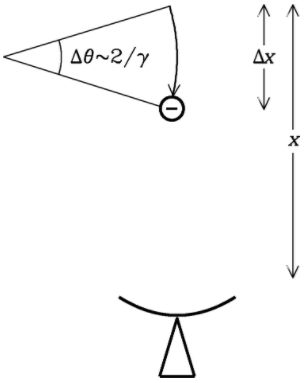
\includegraphics[width=.3\linewidth]{Chapter_2/Figures/NRAO_radio5n4.png}
    \caption[Simple condiguration of the synchrotron source and observer]{\label{fig:nrao_radio5n4}
        This figure shows the simple configuration of synchrotron radio source and the observer.
        During the time $\Delta t$ the electron moves $\Delta x = v\Delta t$ toward the observer, it almost keeps up with the radiation because it is relativistic.
    }
\end{figure}

%Equation(5.54, 55, 56)
\begin{equation}\label{eq:essential_radio5n54}
    \begin{aligned}
        \Delta t\msb{p} &=t(\text{end of observed pulse})-t(\text{start of observed pulse}) \\
                              &=\frac{\Delta x}{v}+\frac{(x-\Delta x)}{c}-\frac{x}{c} \\
                              &= \frac{\Delta x}{v}-\frac{\Delta x}{c}=\frac{\Delta x}{v}\left(1-\frac{v}{c}\right) \quad \ll \quad \frac{\Delta x}{v}=\Delta t
    \end{aligned}
\end{equation}

Replacing the total magnitude field by its perpendicular component $B_{\perp} = B\sin\alpha$ yields

%Equation(5.60)
\begin{equation}\label{eq:essential_radio5n60}
    \Delta t\msb{p} = \frac{1}{\gamma^2 \omega\msb{G} \sin \alpha}
\end{equation}
where $\alpha$ is the pitch angle of the electron.

Thus the synchrotron pulse is spiky with the halfwidth $\frac{\Delta t\msb{p}}{2} < 10^{-10}\,s$ and the time period is $\frac{\gamma}{\nu\msb{G} \brp{=\omega\msb{G} / 2\pi}} > 10^2\,s$ if $\gamma \sim 10^4$ and $B \sim 10\,\mr{\mu G}$ (Figure~\ref{fig:nrao_radio5n5}).

%Figure5.5
\begin{figure}[htbp]
	\centering
	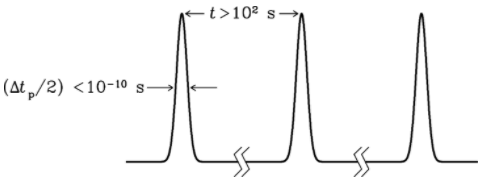
\includegraphics[width=.7\linewidth]{Chapter_2/Figures/NRAO_radio5n5.png}
    \caption[Synchrotron pulse by a single electron]{\label{fig:nrao_radio5n5}
        Synchrotron radiation by a single electron has a narrow pulses.
        Fourier transform of these pulses yields the power spectrum of synchrotron radiation (Equation~\ref{eq:essential_radio5n66}).
    }
\end{figure}


The synchrotron spectrum from a single electron is relatively flat at low frequencies and suddenly falls above

%Equation(5.65)
\begin{equation}\label{eq:essential_radio5n65}
    \nu_{\max} \sim \frac{1}{2 \Delta t\msb{p}} \sim \pi \gamma^2 \nu\msb{G} \sin \alpha \propto \gamma^2 B_{\perp}
\end{equation}

Once we know the pulse shape, we can derive the synchrotron power spectrum of a single electron by the Fourier transform as follows:

%Equation(5.66)
\begin{equation}\label{eq:essential_radio5n66}
    P\brp{\nu} = \frac{\sqrt{3} e^3 B \sin \alpha}{m\msb{e} c^2}\brp{\frac{\nu}{\nu\msb{c}}} \int_{\nu / \nu\msb{c}}^{\infty} K_{5/3}(\eta)\,\rd\eta
\end{equation}
 where $K_{5/3}$ is a modified Bessel function and $\nu_c$ is the critical frequency:

%Equation(5.67)
\begin{equation}\label{eq:essential_radio5n67}
    \nu\msb{c} = \frac{3}{2} \gamma^2 \nu\msb{G} \sin \alpha
\end{equation}

The spectrum shape of a single electron is shown in Figure~\ref{fig:nrao_radio5n6}.

%Figure(5.6)
\begin{figure}[htbp]
	\centering
	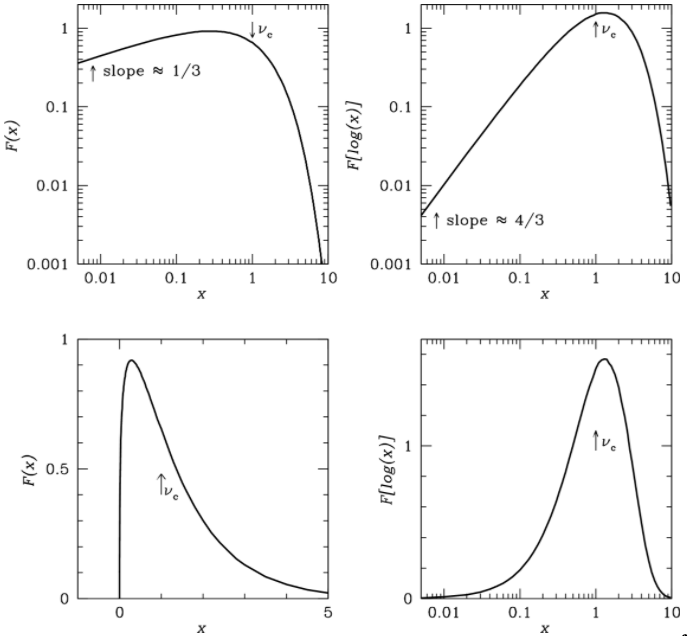
\includegraphics[width=.7\linewidth]{Chapter_2/Figures/NRAO_radio5n6.png}
    \caption[The synchrotron spectrum of a single electron]{\label{fig:nrao_radio5n6}
        These plots show the same function $F\brp{x} \equiv x\int^{\infty}_x K_{5/3}\brp{\eta}\,\rd\eta$ where $x \equiv \nu / \nu\msb{c}$ in different ways.
        In the log-log plot (upper left), we can see the spectral index is $1/3$ less than $x=1$ and it significantly falls above that.
    }
\end{figure}

Indeed, the property by a single electron smears out when we consider an ensemble of electrons due to a wide variety of their energies and pitch angles.


\subsection{Synchrotron Spectra of Optically Thin Radio Sources}\label{subsec:synchrotronspectra_opticallythin}
Here I consider the situation where a synchrotron source is optically thin ($\tau \ll 1$).
In this case, the spectrum of synchrotron radiation is a superposition of the spectra from individual distribution, and its flux density cannot rise faster than $\nu^{1/3}$ at any frequency $\nu$ (Figure~\ref{fig:nrao_radio5n6}).
We usually obtain the spectral index $\alpha\sim-0.75$ ($+$ sign convection) from the observation for most astrophysical sources of synchrotron radiation.
The energy distribution of high energy electrons is roughly a power-law from the theory of Fermi acceleration:

%Equation(5.70)
\begin{equation}\label{eq:essential_radio5n70}
    n(E) \rd E \propto E^{-\delta} \rd E
\end{equation}
where $n\brp{E}\rd E$ is the number of electrons whose energy is between $E$ and $E+\rd E$.

Here, I assume each electron emits the averaged power $\bra{P}$ (Equation~\ref{eq:essential_radio5n38}) with any energy $E$:

%Equation(5.71)
\begin{equation}\label{eq:essential_radio5n71}
    P=-\frac{\rd E}{\rd t}=\frac{4}{3} \sigma\msb{T} \beta^2 \gamma^2 c U_B
\end{equation}

at frequency $\nu \sim \gamma^2\nu\msb{G}$, which is close to the critical frequency $\nu\msb{c}$ (Equation~\ref{eq:essential_radio5n67}).
Then the emission coefficient of synchrotron radiation by an ensemble of electrons is

%Equation(5.73)
\begin{equation}\label{eq:essential_radio5n73}
    j_{\nu} \rd \nu=-\frac{\rd E}{\rd t} n(E) \rd E
\end{equation}
where $E = \gamma m\msb{e} c^2 \sim \brp{\frac{\nu}{\nu\msb{G}}}^{1/2} m\msb{e}c^2$.

Then we can write

%Equation(5.75)
\begin{equation}\label{eq:essential_radio5n75}
    \rd E \approx \frac{m\msb{e} c^2 \nu^{-1 / 2}}{2 \nu\msb{G}^{1 / 2}} \rd \nu
\end{equation}

so,

%Equation(5.76)
\begin{equation}\label{eq:essential_radio5n76}
    j_{\nu} \propto\brp{\frac{4}{3} \sigma\msb{T} \beta^2 \gamma^2 c U_B}\brp{E^{-\delta}}\brp{\frac{m\msb{e} c^2 \nu^{-1 / 2}}{2 \nu\msb{G}^{1 / 2}}}
\end{equation}

To investigate the frequency dependence of the emission coefficient $j_{\nu}$ on the frequency $\nu$ and the magnetic field $B$, I eliminate  $E$ and $\nu\msb{G}$ from the equation above, then

%Equation(5.77) and 5.78
\begin{equation}\label{eq:essential_radio5n77}
    \begin{aligned}
        j_{\nu} & \propto \brp{\frac{\nu}{\nu\msb{G}}} B^2 \brp{\frac{\nu}{\nu\msb{G}}}^{-\delta / 2} \brp{\nu \nu\msb{G}}^{-1 / 2} \propto \brp{\frac{\nu}{B}} B^2 \brp{\frac{\nu}{B}}^{-\delta / 2} \brp{\nu B}^{-1 / 2}\\
                & \propto B^{(\delta+1) / 2} \nu^{(1-\delta) / 2}
    \end{aligned}
\end{equation}

Consequently, the synchrotron radiation in the case of optically thin with the power-law distribution $\brp{n\brp{E} \propto E^{-\delta}}$ also has a power-law distribution and its spectral index $\alpha = \frac{1-\delta}{2}$.

In our galaxy, we observe $\alpha\sim-0.75$ around $1\GHz$ and then $\delta \sim 2.5$.



\subsection{Synchrotron Self-Absorption}\label{synchrotronselfabsorption}

The brightness temperature of synchrotron sources cannot exceed an absolute value at low frequencies, although most radio sources have the emission coefficient $j_{\nu} \propto \nu^{\alpha}$ (mostly in the case of optically thin: $\alpha\sim-0.75$ in $+$ sign convection).
If electrons in LTE and they have the Maxwellian energy distribution, they are thermal sources and their brightness temperatures equal to the electron's kinetic energy.

Here, I describe in the case where electrons are optically thick $\brp{\tau \gg 1}$.
In this case, synchrotron self-absorption happens and the spectral index changes into $\alpha = \frac{5}{2}$.

Firstly, I assume the critical frequency where most of the electrons with energy $E = \gamma m\msb{e} c^2$ emit the synchrotron radiation:

%Equation(5.80)
\begin{equation}\label{eq:essential_radio5n80}
    \nu_{\mathrm{c}} \sim \frac{\gamma^{2} e B}{2 \pi m_{\mathrm{e}} c}
\end{equation}

In the relativistic gas, the ratio between specific heats at constant pressure and volume is $\frac{c\msb{P}}{c\msb{V}}=\frac{4}{3}$ (nonrelativistic case: $\frac{5}{3}$).
So the relation between electron energy $E$ and electron temperature $T\msb{e}$ is

%Equation(5.82)
\begin{equation}\label{eq:essential_radio5n82}
    E=3 k T\msb{e}
\end{equation}

Thus, the effective temperature of relativistic electrons is defined below:

%Equation(5.83)
\begin{equation}\label{eq:essential_radio5n83}
    T\msb{e} \equiv \frac{E}{3 k}=\frac{\gamma m\msb{e} c^2}{3 k}
\end{equation}

Eliminating $\gamma$ from Equation~\ref{eq:essential_radio5n80} and~\ref{eq:essential_radio5n83} yields

%Equation(5.84)
\begin{equation}\label{eq:essential_radio5n84}
    T\msb{e} \approx \brp{\frac{2 \pi m\msb{e} c \nu}{e B}}^{1 / 2} \frac{m\msb{e} c^2}{3 k} \sim 1.18 \times 10^6\brp{\frac{\nu}{\mr{Hz}}}^{1/2}\brp{\frac{B}{\mr{gauss}}}^{-1/2}
\end{equation}

At sufficiently low frequency, the brightness temperature $T\msb{b}$ approaches the effective electron temperature $T\msb{e}$, and radio sources become opaque.
In the Rayleigh-Jeans limit, we can write $T\msb{b}$ as follows:

%Equation(5.87)
\begin{equation}\label{eq:essential_radio5n87}
    T\msb{b} \equiv \frac{I_{\nu}c^2}{2k\nu^2}
\end{equation}
where $I_{\nu}$ is the spectral brightness.

Substituting $T\msb{b} \sim T\msb{e}$ and Equation~\ref{eq:essential_radio5n84} yields:

%Equation(5.88)
\begin{equation}\label{eq:essential_radio5n88}
    I_{\nu} \sim \frac{2kT\msb{e}\nu^2}{c^2} \propto \nu^{1/2}\nu^2 B^{-1/2} = \nu^{5/2} B^{-1/2}
\end{equation}

Therefore, the self-absorbed synchrotron source has a spectral index $\alpha\sim\frac{5}{2}$ $\brp{S\brp{\nu} \sim \nu^{5/2}}$, which is independent of the slope $\delta$.

The spectrum of a homogeneous cylindrical synchrotron source is showed in Figure~\ref{fig:nrao_radio5n7}.

%Figure(5.7)
\begin{figure}[htbp]
	\centering
	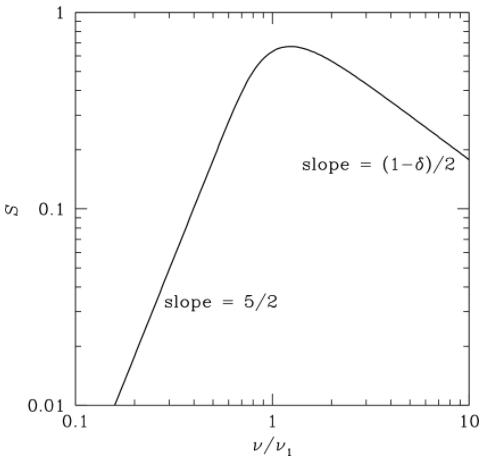
\includegraphics[width=.6\linewidth]{Chapter_2/Figures/NRAO_radio5n7.png}
    \caption[The spectrum of synchrotron radiation]{\label{fig:nrao_radio5n7}
        This figure shows the synchrotron spectrum.
        $\nu_1$ is the frequency at which $\tau=1$.
        The spectral index at the frequency $\nu$ above $\nu_1$ is $\brp{1-\delta}/2$.
        At lower frequencies less than $\nu_1$, we can see the synchrotron self-absorption with the slope $5/2$.
    }
\end{figure}

However, real radio sources have more complex shapes because they have nonuniform magnetic fields and electron energy distributions (Figure~\ref{fig:nrao_radio5n8}).

%Figure(5.8)
\begin{figure}[htbp]
	\centering
	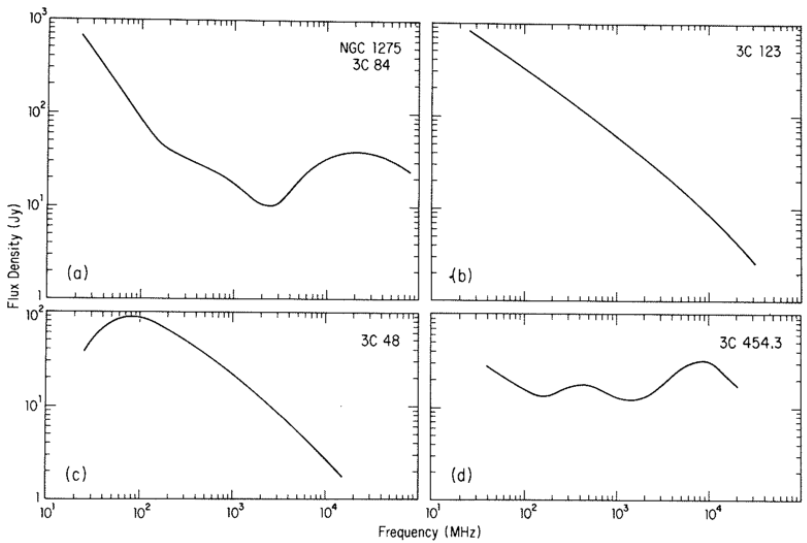
\includegraphics[width=.9\linewidth]{Chapter_2/Figures/NRAO_radio5n8.png}
    \caption[The spectrum of synchrotron radiation from real sources]{\label{fig:nrao_radio5n8}
        These plots show the radio spectra at low frequencies $\brp{10 \sim 10^5\MHz}$.
        Since real radio sources do not have uniform structures, these spectra look quite different from the uniform case (Figure~\ref{fig:nrao_radio5n7})
    }
\end{figure}

	\chapter{Data}\label{chap:data}
\begin{chapabstract}

In this chapter, I describe the dataset used for our study.
In Section~\ref{sec:HerschelReferenceSurvey}, I introduce the Herschel Reference Survey Catalog \citep{Boselli2010}.
Here, I explain how they choose galaxies for the catalog and previous studies for them.
In Section~\ref{sec:gleamsurvey}, I introduce the GaLactic Extragalactic All-sky MWA survey, which we obtained the radio data for galaxy samples.

\end{chapabstract}

\section{Herschel Reference Survey (HRS)}\label{sec:HerschelReferenceSurvey}
In this section, I introduce the Herschel Reference Survey (HRS) catalog \citep{Boselli2010} from which we selected galaxy samples.
This survey is one of the Herschel guaranteed time key projects, and originally it was compiled for understanding dust properties and the interstellar medium in nearby galaxies.
The catalog is publicly available and contains 322 galaxies selected with three criteria as follows:

\begin{enumerate}
    \item Volume-limited:\\
        They choose galaxies whose distance from the earth is between $15$ and $25\,\mr{Mpc}$.
        This limitation reduces the distance uncertainty due to the galaxy peculiar motions and the selection effect due to the high-$z$ galaxies.
        The lower limit ($15\,\mr{Mpc}$) also helps us to observe sources within reasonable exposure time because very close galaxies us are extended, and we need too much time for the observation.
    \item $K$-band selection:\\
        They choose galaxies whose 2MASS $K$-band total magnitudes are brighter than $12\,\mr{mag}$ for star-forming and peculiar galaxies (Sa-Sd-Im-BCD), and $8.7\,\mr{mag}$ for quiescent galaxies (E, S0, S0a).
        If there are galaxies whose $K$-band magnitude darker than those values, their measurements are not regarded as accurate photometry because of not enough exposure time.
        The reason why they have selected quiescent galaxies with the more stringent $K$-band selection criteria is these galaxies are expected to have low dust contents, and it is difficult to detect within the reasonable exposure time.
    \item High galactic latitude:\\
        They choose galaxies whose galactic latitude is high enough to minimize the contamination from the galactic center ($b > +55^{\circ}$).
        Also, they select galaxies with the low galactic extinction ($A\msb{B} < 0.2$; \citealt{Schlegel1998}).
\end{enumerate}

The selected galaxies locate in the sky region between $10\msu{h}17\msu{m}< \mr{R.A.}(2000) < 14\msu{h}43\msu{m}$ and $-6^{\circ} < \mr{decl.} < 60^{\circ}$ (Figure~\ref{fig:Boselli2010_figure1}).
HRS galaxies span a wide range of the galaxy density environment from the center of the Virgo cluster to the isolated region.
As a definition, we can regard the HRS sample as an ideal one for studying the galaxy environment.

\begin{figure}[htbp]
	\centering
	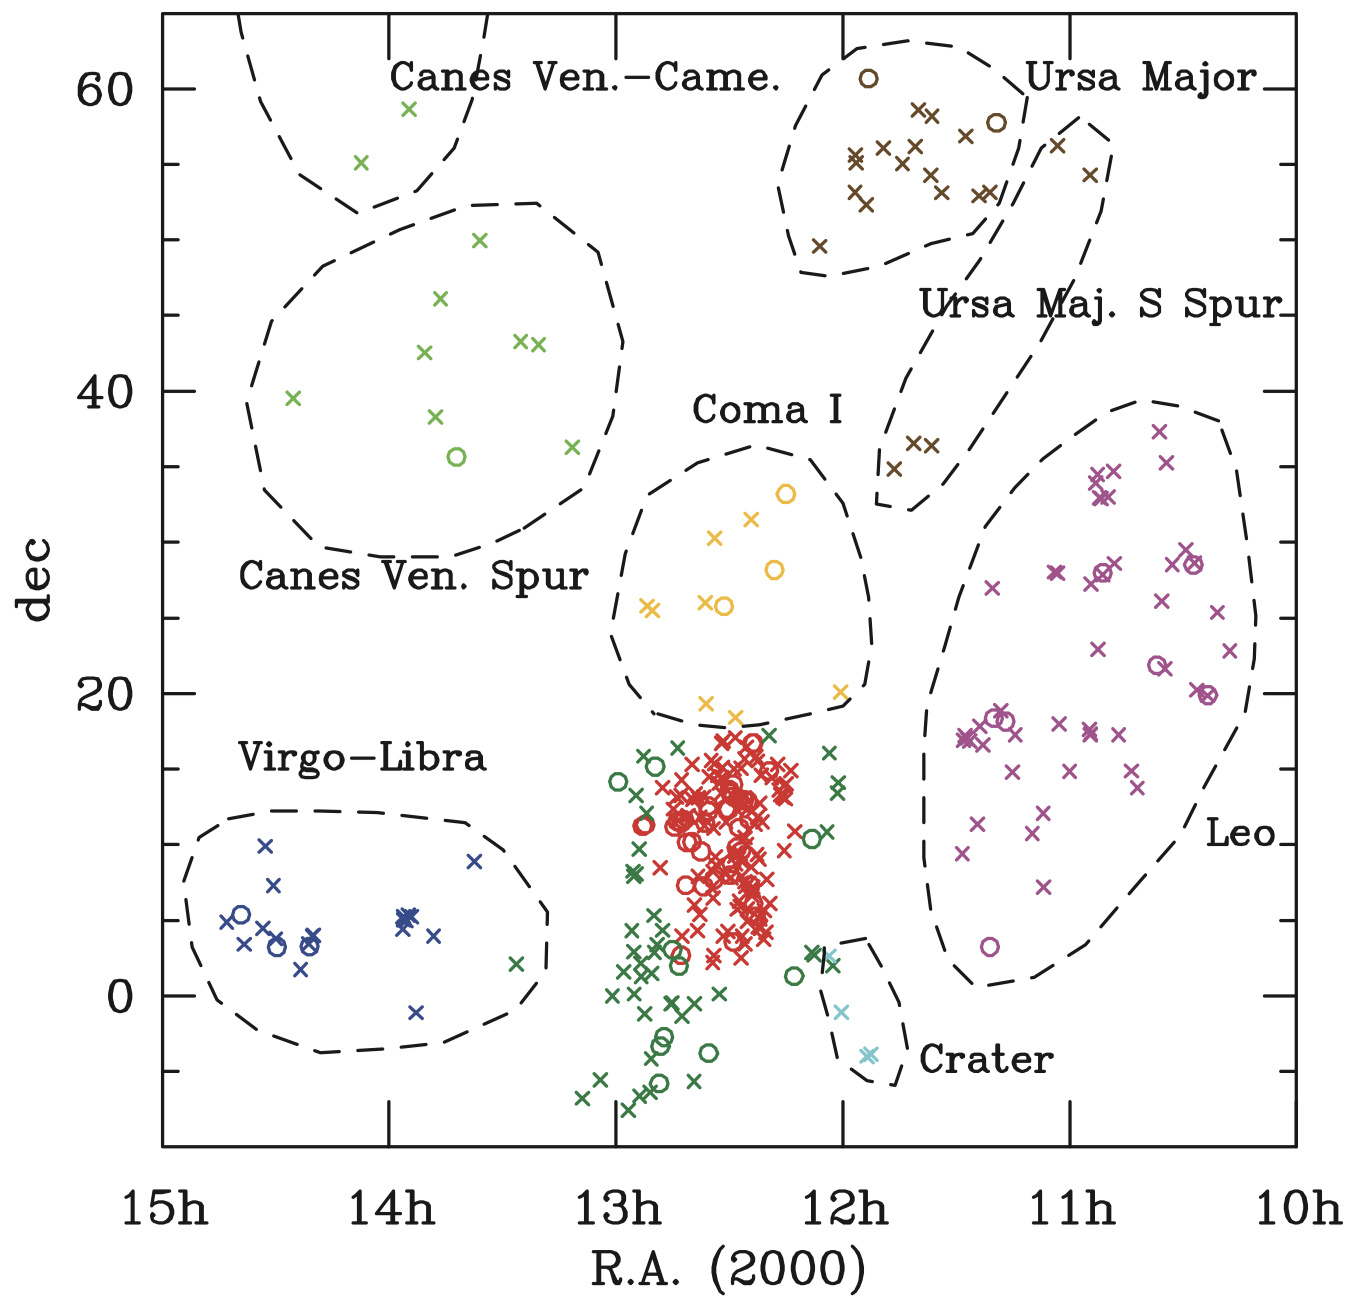
\includegraphics[width=.7\linewidth]{Chapter_3/Figures/Boselli2010_Figure1.png}
    \caption[Reprint from Boselli et al. 2010 (Figure~1)]{\label{fig:Boselli2010_figure1}
        (Reprint from Boselli et al. 2010, Figure~1)\\
        This figure shows the sky distribution of HRS galaxy samples.
        They show the early-type galaxies (E, S0, S0a) and late-type galaxies with circles and crosses, respectively.
        Dashed circles represents the different cloud regions. Each name of the cloud is shown close to each region.
        The red and dark green markers are Virgo galaxies (red: Virgo center, dark green: its outskirts).
    }
\end{figure}

In addition to a wide range of the environment, HRS galaxies distribute a wide range of galaxy morphology (Figure~\ref{fig:Boselli2010_figure2}).

\begin{figure}[htbp]
	\centering
	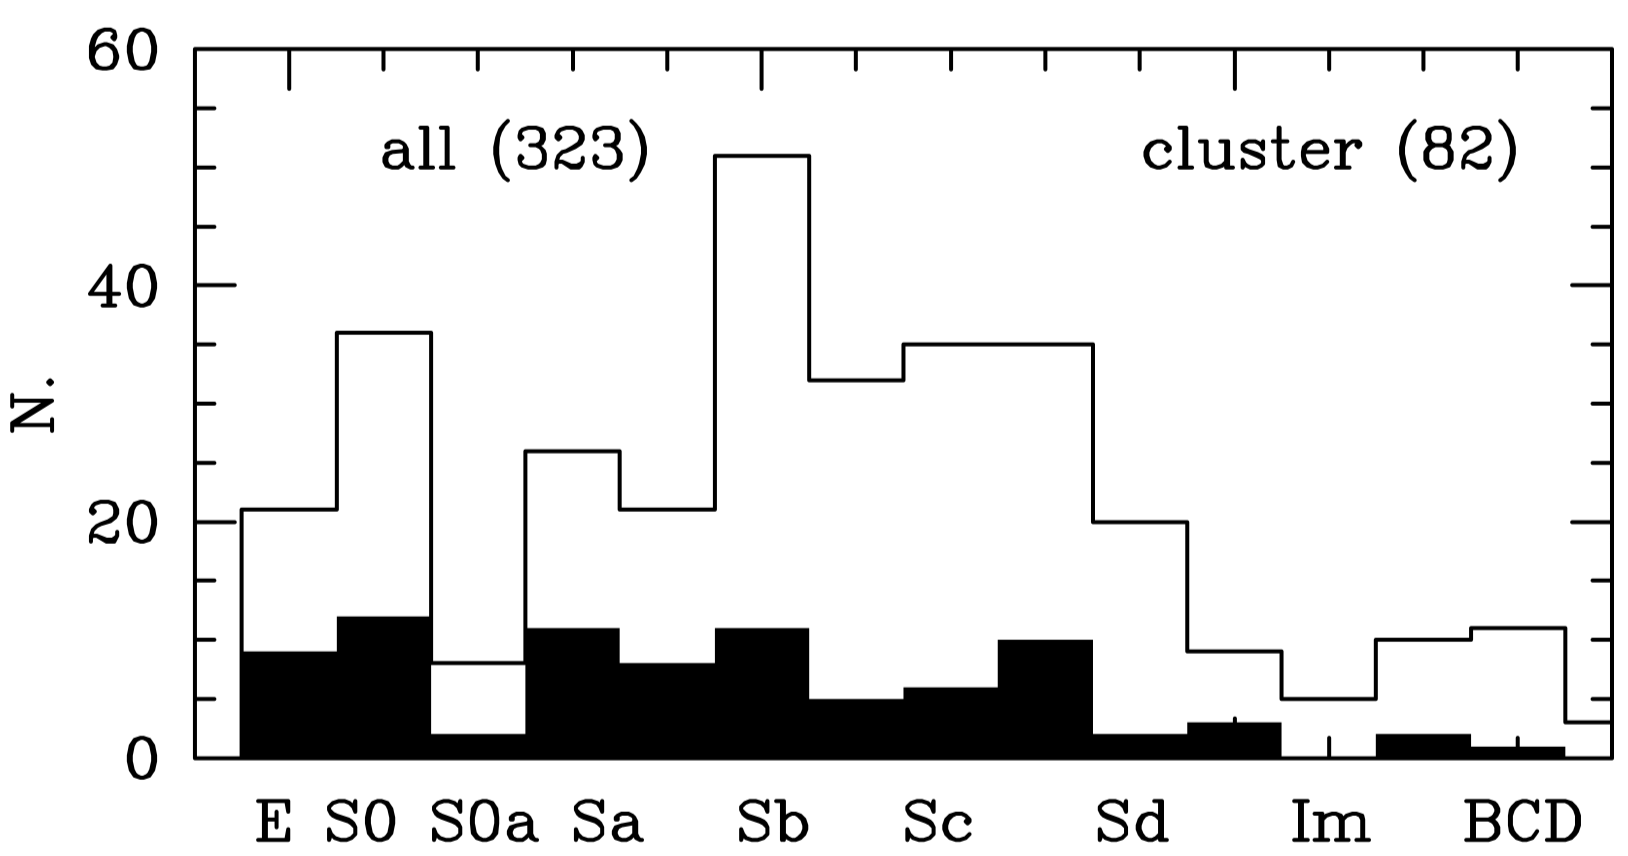
\includegraphics[width=.8\linewidth]{Chapter_3/Figures/Boselli2010_Figure2.png}
    \caption[Reprint from Boselli et al. 2010 (Figure~2)]{\label{fig:Boselli2010_figure2}
        (Reprint from Boselli et al. 2010, Figure~2)\\
        This figure shows the distribution in the morphology-type of HRS galaxies.
        The shaded histogram represents the distribution in it of only the cluster sample.
        Here, the cluster sample composed of HRS galaxies located in the Virgo A and B clouds.
    }
\end{figure}

Since HRS galaxies are supposed to be well-represented for the whole galaxy population located in the local universe, investigating their physical properties is crucial to understand them.
After \citet{Boselli2010} published the HRS catalog, many studies investigating the physical properties for HRS galaxies have been done until now.
Here, I introduce some of the studies for the HRS sample.
\citet{Cortese2012} investigated their UV and optical properties using the Galaxy Evolution Explorer ({\it GALEX\/};~\citealt{Martin2005}) and SDSS-DR7 \citep{Abazajian2009}.
\citet{Boselli2014} studied their cold gas properties with $^{12}\mr{CO}\brp{1-0}$ observed by the Kitt Peak 12m radio telescope and obtained from the literature data.
They also investigate the \nh~gas obtained from The Arecibo Legacy Fast ALFA (ALFALFA;~\citealt{Giovanelli2005, Haynes2011}) survey.
\citet{Ciesla2014} executed the SED fitting for HRS galaxies with Code Investigating GALaxy Emission (CIGALE;~\citealt{Noll2009}).

Thanks to all of the previous research about the HRS sample, they are well-studied from the X-ray to the radio emission at $1.5\GHz$.
However, the low-frequency around $100\MHz$ is not examined so far.
Since we extend the wavelength range of the HRS sample to around $100\MHz$, in this study, we focus on a subsample of HRS galaxies whose counterpart is detected by the latest low-frequency survey (Section~\ref{sec:gleamsurvey}).



\section{GLEAM survey}\label{sec:gleamsurvey}

In this section, I introduce the GaLactic Extragalactic All-sky MWA (GLEAM) survey \citep{Hurley-Walker2017a} which we obtained the radio continuum data from.
This survey was operated by the Murchison Widefield Array (MWA) telescope in Western Australia \citep{Tingay2013a}.
It observed a whole southern sky and a northern sky up to $+30^{\circ}$ ($\sim$25,000 $\mathrm{\deg}^2$;~Figure~\ref{fig:HurleyWalker2017_figure11}).
The catalog from this survey is a publicly-available and contains 307,455 detected radio sources with fluxes at 20 narrow bands between $72$ and $231\MHz$ (each band has $7.68\MHz$ band width).
The sensitivity and angular resolution at $200\MHz$ are $\sim 7\,\mr{mJy}$ and $\sim 2\,\mr{arcmin}$ respectively.
The completeness of this survey at $200\MHz$ is $90\%$ at $\sim 170\mr{mJy}$.
Since this survey allows us to examine the low-frequency spectral energy distribution accurately with its 20 narrow bands, we adopt the radio source catalog for our study.

\begin{figure}[htbp]
	\centering
	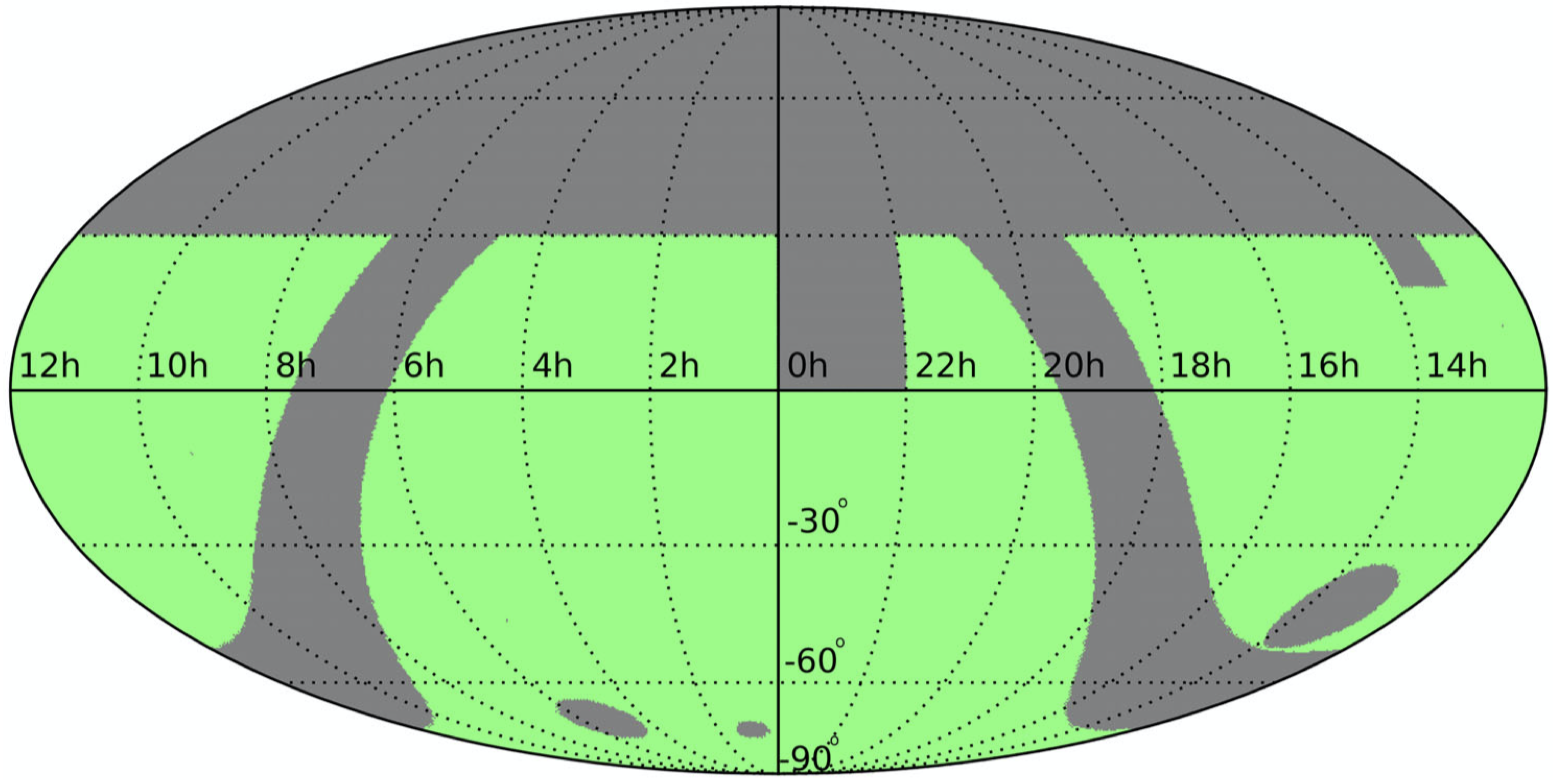
\includegraphics[width=.7\linewidth]{Chapter_3/Figures/HurleyWalker_Figure11.png}
    \caption[Reprint from Hurley-Walker et al. 2017 (Figure~11)]{\label{fig:HurleyWalker2017_figure11}
        (Reprint from Hurley-Walker et al. 2017, Figure~11)\\
        This figure shows the observed area by the GLEAM survey (green shaded region).
        \citet{Hurley-Walker2017a} exclude several regions intentionally to minimize the contamination:
        Galactic plane (Absolute Galactic latitude $<10^{\circ}$),
        Ionospherically distorted ($0^{\circ} < \mr{Dec} < +30^{\circ}\ \mr{and}\ 22\msu{h} < \mr{R.A.} < 0\msu{h}$),
        Centaurus A ($13\msu{h}25\msu{m}28\msu{s}\ -43^{\circ}01'09'',\,r=9^{\circ}$),
        Sidelobe reflection of Cen A ($20^{\circ} < \mr{Dec} < +30^{\circ}\ \mr{and}\ 13\msu{h}07\msu{m} < \mr{R.A.} < 13\msu{h}53\msu{m}$),
        Large Magellanic Cloud ($05\msu{h}23\msu{m}35\msu{s}\ -69^{\circ}45'22'',\,r=5.5^{\circ}$) and Small Magellanic Cloud ($00\msu{h}52\msu{m}38\msu{s}\ -72^{\circ}48'01'',\,r=2.5^{\circ}$).
    }
\end{figure}






%\bibliographystyle{mnras}
%%\bibliography{example} % if your bibtex file is called example.bib
%\bibliography{masterthesis}

	\chapter{Methods}\label{chap:methods}
\begin{chapabstract}

Intro intro intro intro.

\end{chapabstract}

\section{Cross Matching}\label{sec:crossmatching}
Although HRS galaxies have been studied in multi-wavelength observations, their spectral energy distribution around $100\MHz$ is not well-understood, where the contribution from synchrotron radiation is much more significant than from free-free emission \citep{Condon1992a}.
Here, I provide a procedure to cross-matching with two different catalogs I have mentioned in the previous chapter.
Cross-matching is the method widely used in astronomy to obtain additional information from other surveys or catalogs by matching coordinates of each galaxy or blob source within a specific error (e.g., $\sim 1\,\mr{arcsec}$).
For executing this method for the HRS and the GLEAM survey catalog, we use Tool for OPerations on Catalogues And Tables (TOPCAT\@; \citealt{Taylor2009}).
TOPCAT is popular and an useful tool for dealing with catalogs and tables, and it allows us to do the cross-matching easily, even more than two catalogs.

Initially, we assume a $10\,\mr{arcsec}$ error radius for the cross-matching since it is equivalent to the value of $95\%$ error for the astrometry in the GLEAM survey (Section 4.5.5 in \citealt{Hurley-Walker2017a}).
This matching results in a total of 18 galaxies which are identified to have a radio counterpart.
To assess the matching, we compare a separation of counterparts from the center of galaxies with coordinate uncertainties in the GLEAM catalog.
For these galaxies, we find 15 of them have a separation within a 95\% error radius, and others do not.
Although three of them have a larger separation compared to the error radius, we conclude that the matching for all 18 galaxies is correct by the checking of galaxy images (Appendix~\ref{chap:galaxyimages}).
In this paper, we regard a radio blob as a counterpart if the brightest part of each blob where the inside of the contour nearest to the center, is surrounded by the D25 radius (the isophotal optical size at $25\,\mr{mag}\arcs^{-2}$; \citealt{Boselli2010}).

Next, we extend the error radius up to $120\arcs$, which is corresponding to the angular resolution of the GLEAM survey at $200\MHz$.
This is because the radio sources are blurred due to the angular resolution of the GLEAM survey and the location of them might be shifted.
We know $120\arcs$ error radius is quite big for the matching, but this trial gives us the inspiration for the cross-matching with blurred radio sources in the future study.
The cross-matching with the error of $120\arcs$ suggests that there are 25 new galaxies have a potential counterpart.
To assess these matching, we look at galaxy images one by one (All galaxy images are in Appendix~\ref{chap:galaxyimages}).
With the same condition mentioned above, we identify 21 matches for these galaxies.

Although we have identified a total of 39 matches in the same way, there are six suspicious matches because of interacting counterparts (HRS4, 216, 244, 284) and quite large separations (HRS200, 295) (Figure~\ref{fig:galaxyimages_suspicious}).
For these galaxies, we flag them as suspicious matches, and we do not use them for further analysis.
The distribution of separations for galaxies showed in Figure~\ref{fig:separation}.

\begin{figure}[htbp]
	\centering
	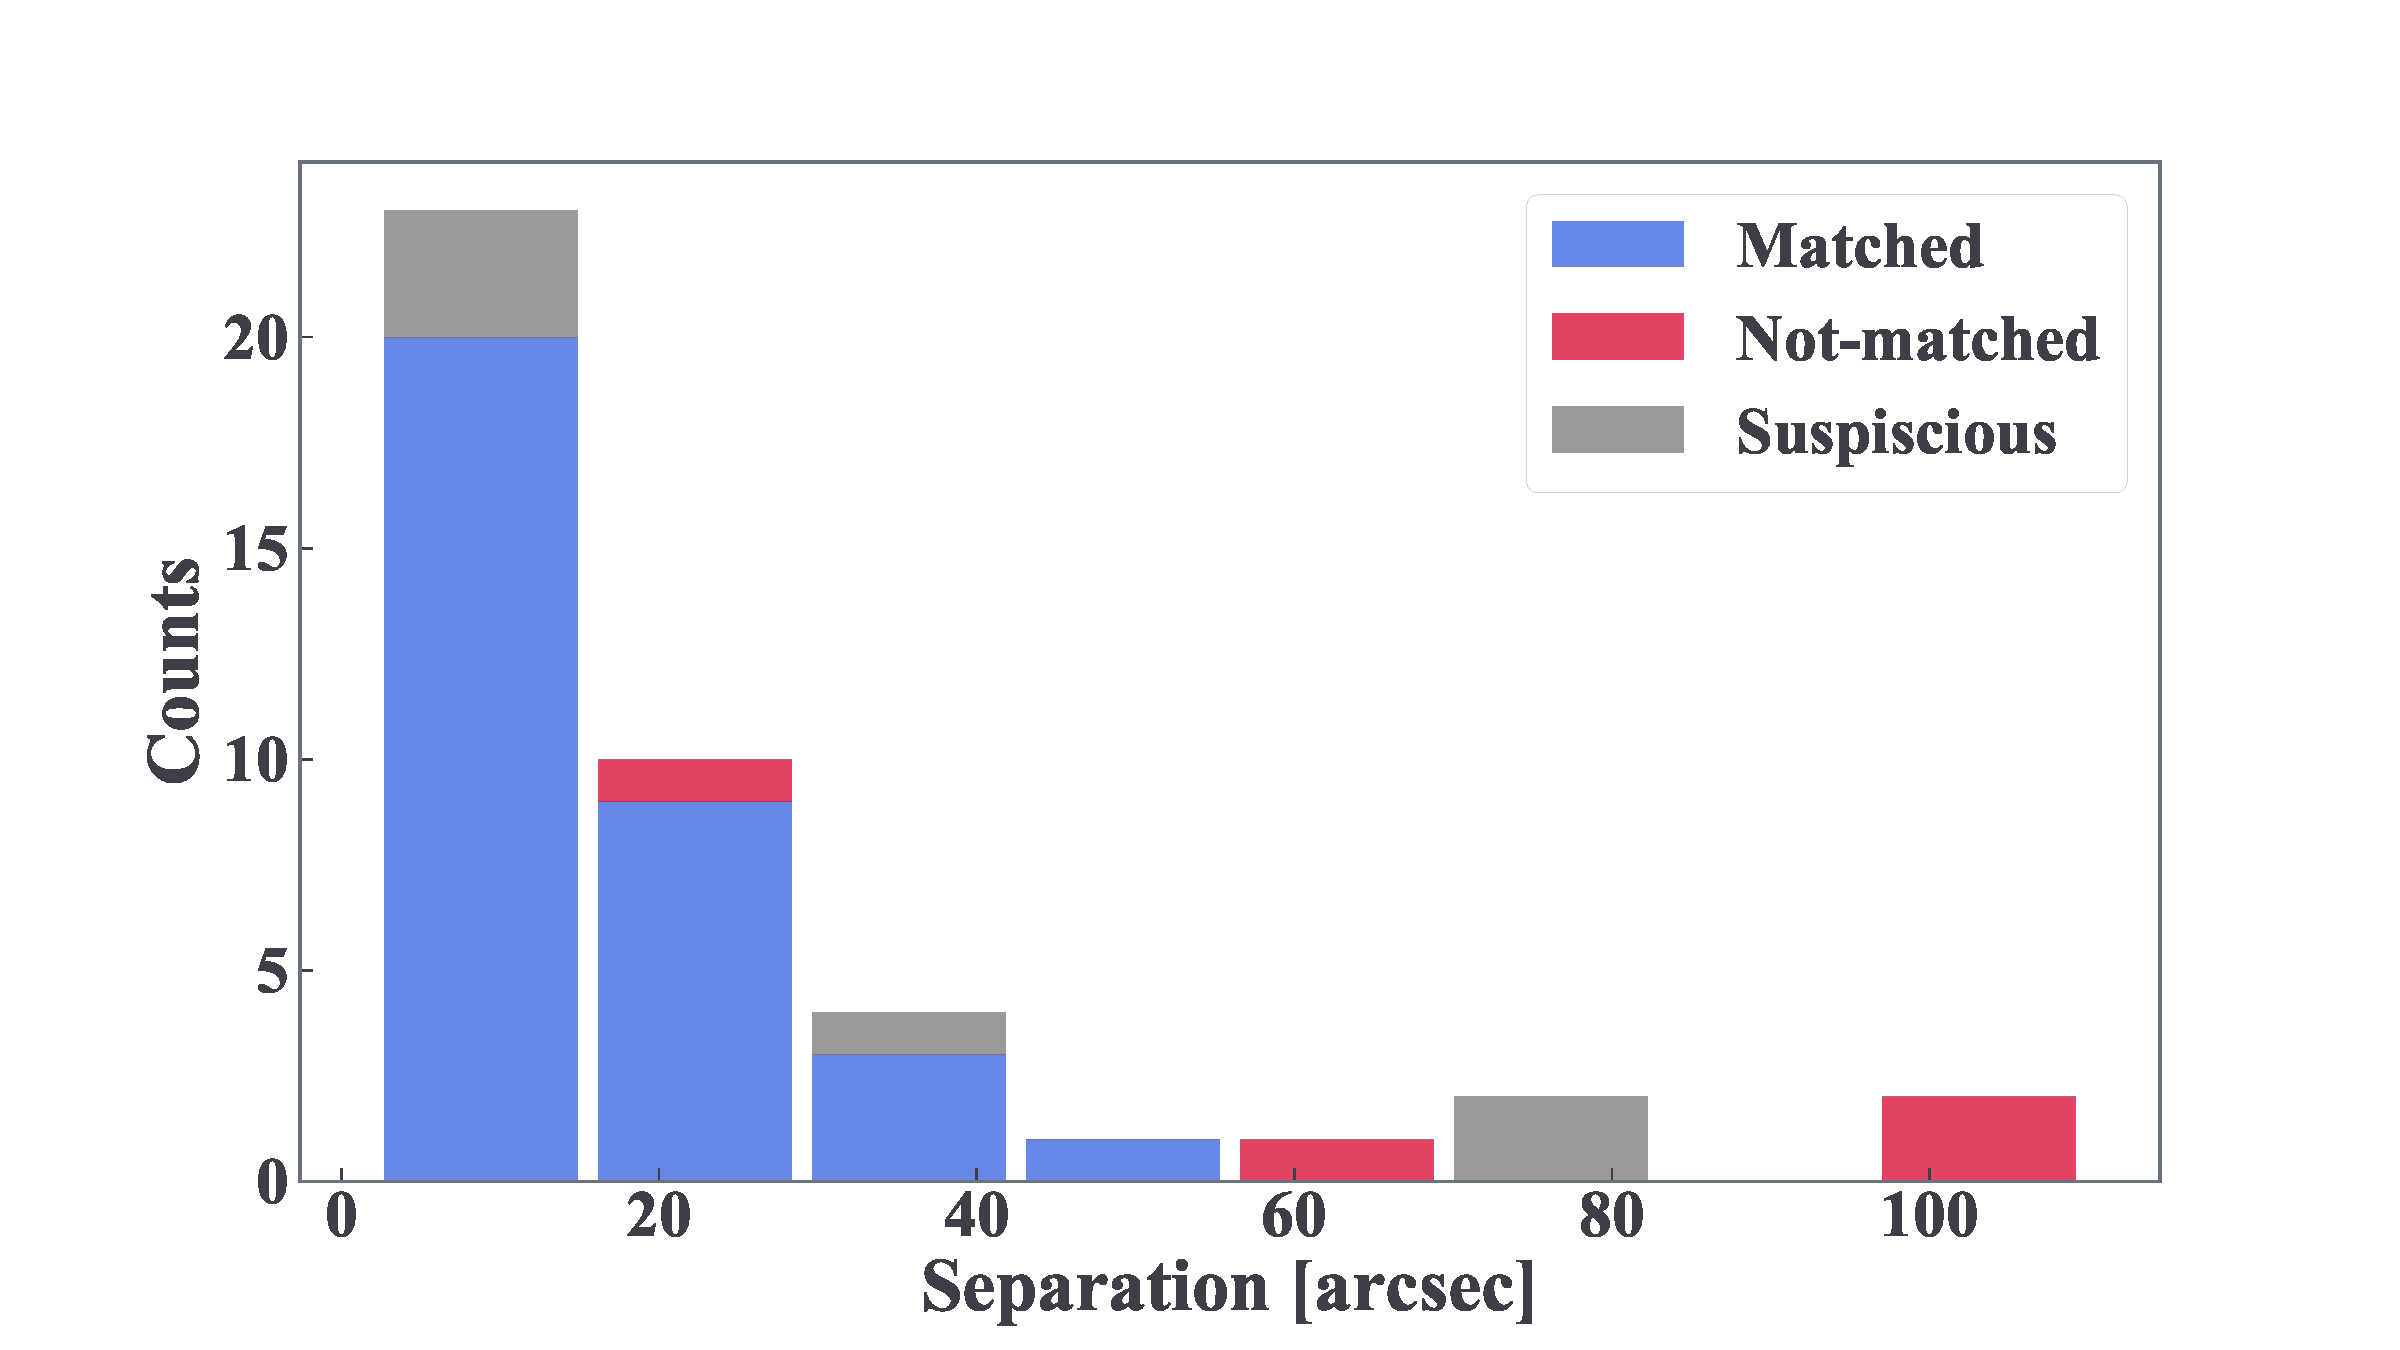
\includegraphics[width=.8\linewidth]{Chapter_4/Figures/Method_separation.pdf}
    \caption[Separation from the cross-matching]{\label{fig:separation}
        This figure shows the distribution of separations.
        Here we put 43 galaxies and color sorted based on the result.
        The blue bar shows galaxies identified to have a radio counterpart, red one does galaxies determined not to have a counterpart, and gray for the suspicious galaxies.
        Most of the matched samples are distributed within a $40\,\mr{arcsec}$ error radius.
    }
\end{figure}

We put all galaxy images cross-matched within $120\,\mr{arcsec}$ in Appendix~\ref{chap:galaxyimages}.



\section{Reduce galaxy samples for the secure analysis}\label{sec:reducegalaxysamples}

In this section, we show some steps for selecting galaxies to do a secure analysis.
Since we focus on the relation of galaxy radio emission with star formation activities, we should clarify the radio source and be sure that they are not originally from other sources rather than the star formation.
The radio emission arisen from the star formation activities should be proportional to the SFR in a galaxy \citep{Condon1992a, Murphy2011}.
However, elliptical galaxies have a stronger radio emission against their star formation, in this case their radio emission would be emitted by non star-forming sources.
These radio sources are considered as Active Galactic Nuclei (AGN), which emits strong radio emission due to the baryon accretion into the supermassive black hole at the center of galaxies irrelevant to the star formation \citep[e.g.,][]{Urry1995, Padovani2017}.
According to the morphology of galaxies \citep{Cortese2012}, we identify four elliptical galaxies (HRS49, 138, 178, 241) and not use for further calculation and discussion.
%With these operations, we finally find that there are 37 HRS galaxies are available for further analysis.

After this galaxy selection, we obtain 29 galaxies with a reliable radio counterpart arisen from the star formation activity.

As a next step, we evaluate the signal to noise ratio (SNR) of radio emission at each MWA band.
For reducing the uncertainty caused by observational errors, we assess the peak flux at each narrow band by comparing it to the local noise level and adopt flux values whose SNR is higher than five.
This analysis results in a total of 11 galaxies have no radio fluxes whose SNR is higher than the criterion.
The reason why these radio sources are detected, although they do not have any fluxes with higher SNR, is \citet{Hurley-Walker2017a} determine the detection based on the SNR in the stacking images ($170-231\MHz$).
%\vspace{0.3cm}\\

Finally, after the cross-matching and these procedures, we confirm 18 HRS galaxies are the samples available for further analysis.
The overview of 18 samples is tabled in Appendix~\ref{chap:galaxysamples}.



\section{Calculating the $\qn$ parameter}\label{subsec:calculatingq}
In this section, I introduce the method to calculate $\qn$ parameter for each galaxy.
The definition of this parameter here is given on the following equation \citep[e.g.][]{Helou1985, Bell2003, CalistroRivera2017a}:

\begin{equation}\label{eq:q_def}
    \qn \equiv \log\brp{\frac{L\msb{8-1000\,\mu m}\ /\ 3.75 \times 10^{12}}{{\rm erg\,s^{-1}\,Hz^{-1}}}} - \log\brp{\frac{L_{\mr{Radio},\,\nu}}{{\rm erg\,s^{-1}\,Hz^{-1}}}}
\end{equation}
where $L\msb{8-1000\,\mu m}$ is the total rest-frame infrared luminosity among $8 - 1000\,\mr{\mu m}$, which reflects the total dust luminosity, and $3.75\times10^{12}$ is equivalent to the frequency of $80\,\mr{\mu m}$ for correcting the dimension.

Although \citet{Ciesla2014} have already derived the total IR luminosity for most HRS galaxies using the SED fitting, one of our galaxy samples (HRS163) does not have the value because of the lack of the reliable mid IR flux from {\it Spitzer\/} telescope.
For consistency, we adopt the total IR luminosity calculated from the same method for all galaxy samples.
To calculate the total IR luminosity, we refer to \citet{Galametz2013}, which derive the calibration relation between combining monochromatic IR luminosities and the total IR luminosity.
We show the procedure to calculate total IR luminosity in the next section.



\section{Total IR luminosity}\label{sec:tirluminosity}
In this section, I present how to calculate the total IR luminosity.
For the method of calculating total IR luminosity, we refer to \citet{Galametz2013}, which shows the empirical relations to estimate total IR from {\it Spitzer\/} ($24, 70\micron$) and {\it Herschel\/} bands ($100, 160, 250\micron$).
HRS galaxies have flux data from the Multiband Imaging Photometry for {\it Spitzer\/} (MIPS;~\citealt{Rieke2004, Bendo2012}), the {\it Herschel\/}/PACS ($100,\,160\micron$; \citealt{Cortese2014c}) and the {\it Herschel\/}/SPIRE ($250\micron$; \citealt{Ciesla2012a}).

\citet{Galametz2013} derived the calibration equation below:

\begin{equation}\label{eq:galametz}
    L\msb{3-1100\mr{\mu m}} = \sum c_i \nu L_{\nu}\left(i\right)
\end{equation}
where $L\msb{3-1100\,\mu m}$ is the total IR luminosity in the frequency range from 3 to 1100 $\mr{\mu m}$, $c_i$ is the coefficients at $i = 24,\,70,\,100,\,160,\,250\,\mathrm{\mu m}$, and $L_{\nu}$ is the luminosity at the frequency $\nu$ corresponds to a specific wavelength $i$.
For deriving $L_{\nu}$, we calculate it from fluxes and the distance to each galaxy.
We refer to \citet{Cortese2012} for obtaining galaxy distances.

\citet{Galametz2013} derived the conversion equation with at least two bands.
Therefore, we can estimate total IR luminosities even if galaxies are lack of a few fluxes.
Since several calculations in the following sections require the total IR luminosity among $8 - 1000\micron$ ($L\msb{8-1000\micron}$), we recalibrate this luminosity by multiplying the constant value (0.88) in \citet{Takeuchi2005}.

The total IR luminosity calculated here is consistent with that of \citet{Ciesla2014} within factor 2 (Figure~\ref{fig:tircomparison}).

\begin{figure}[htbp]
	\centering
	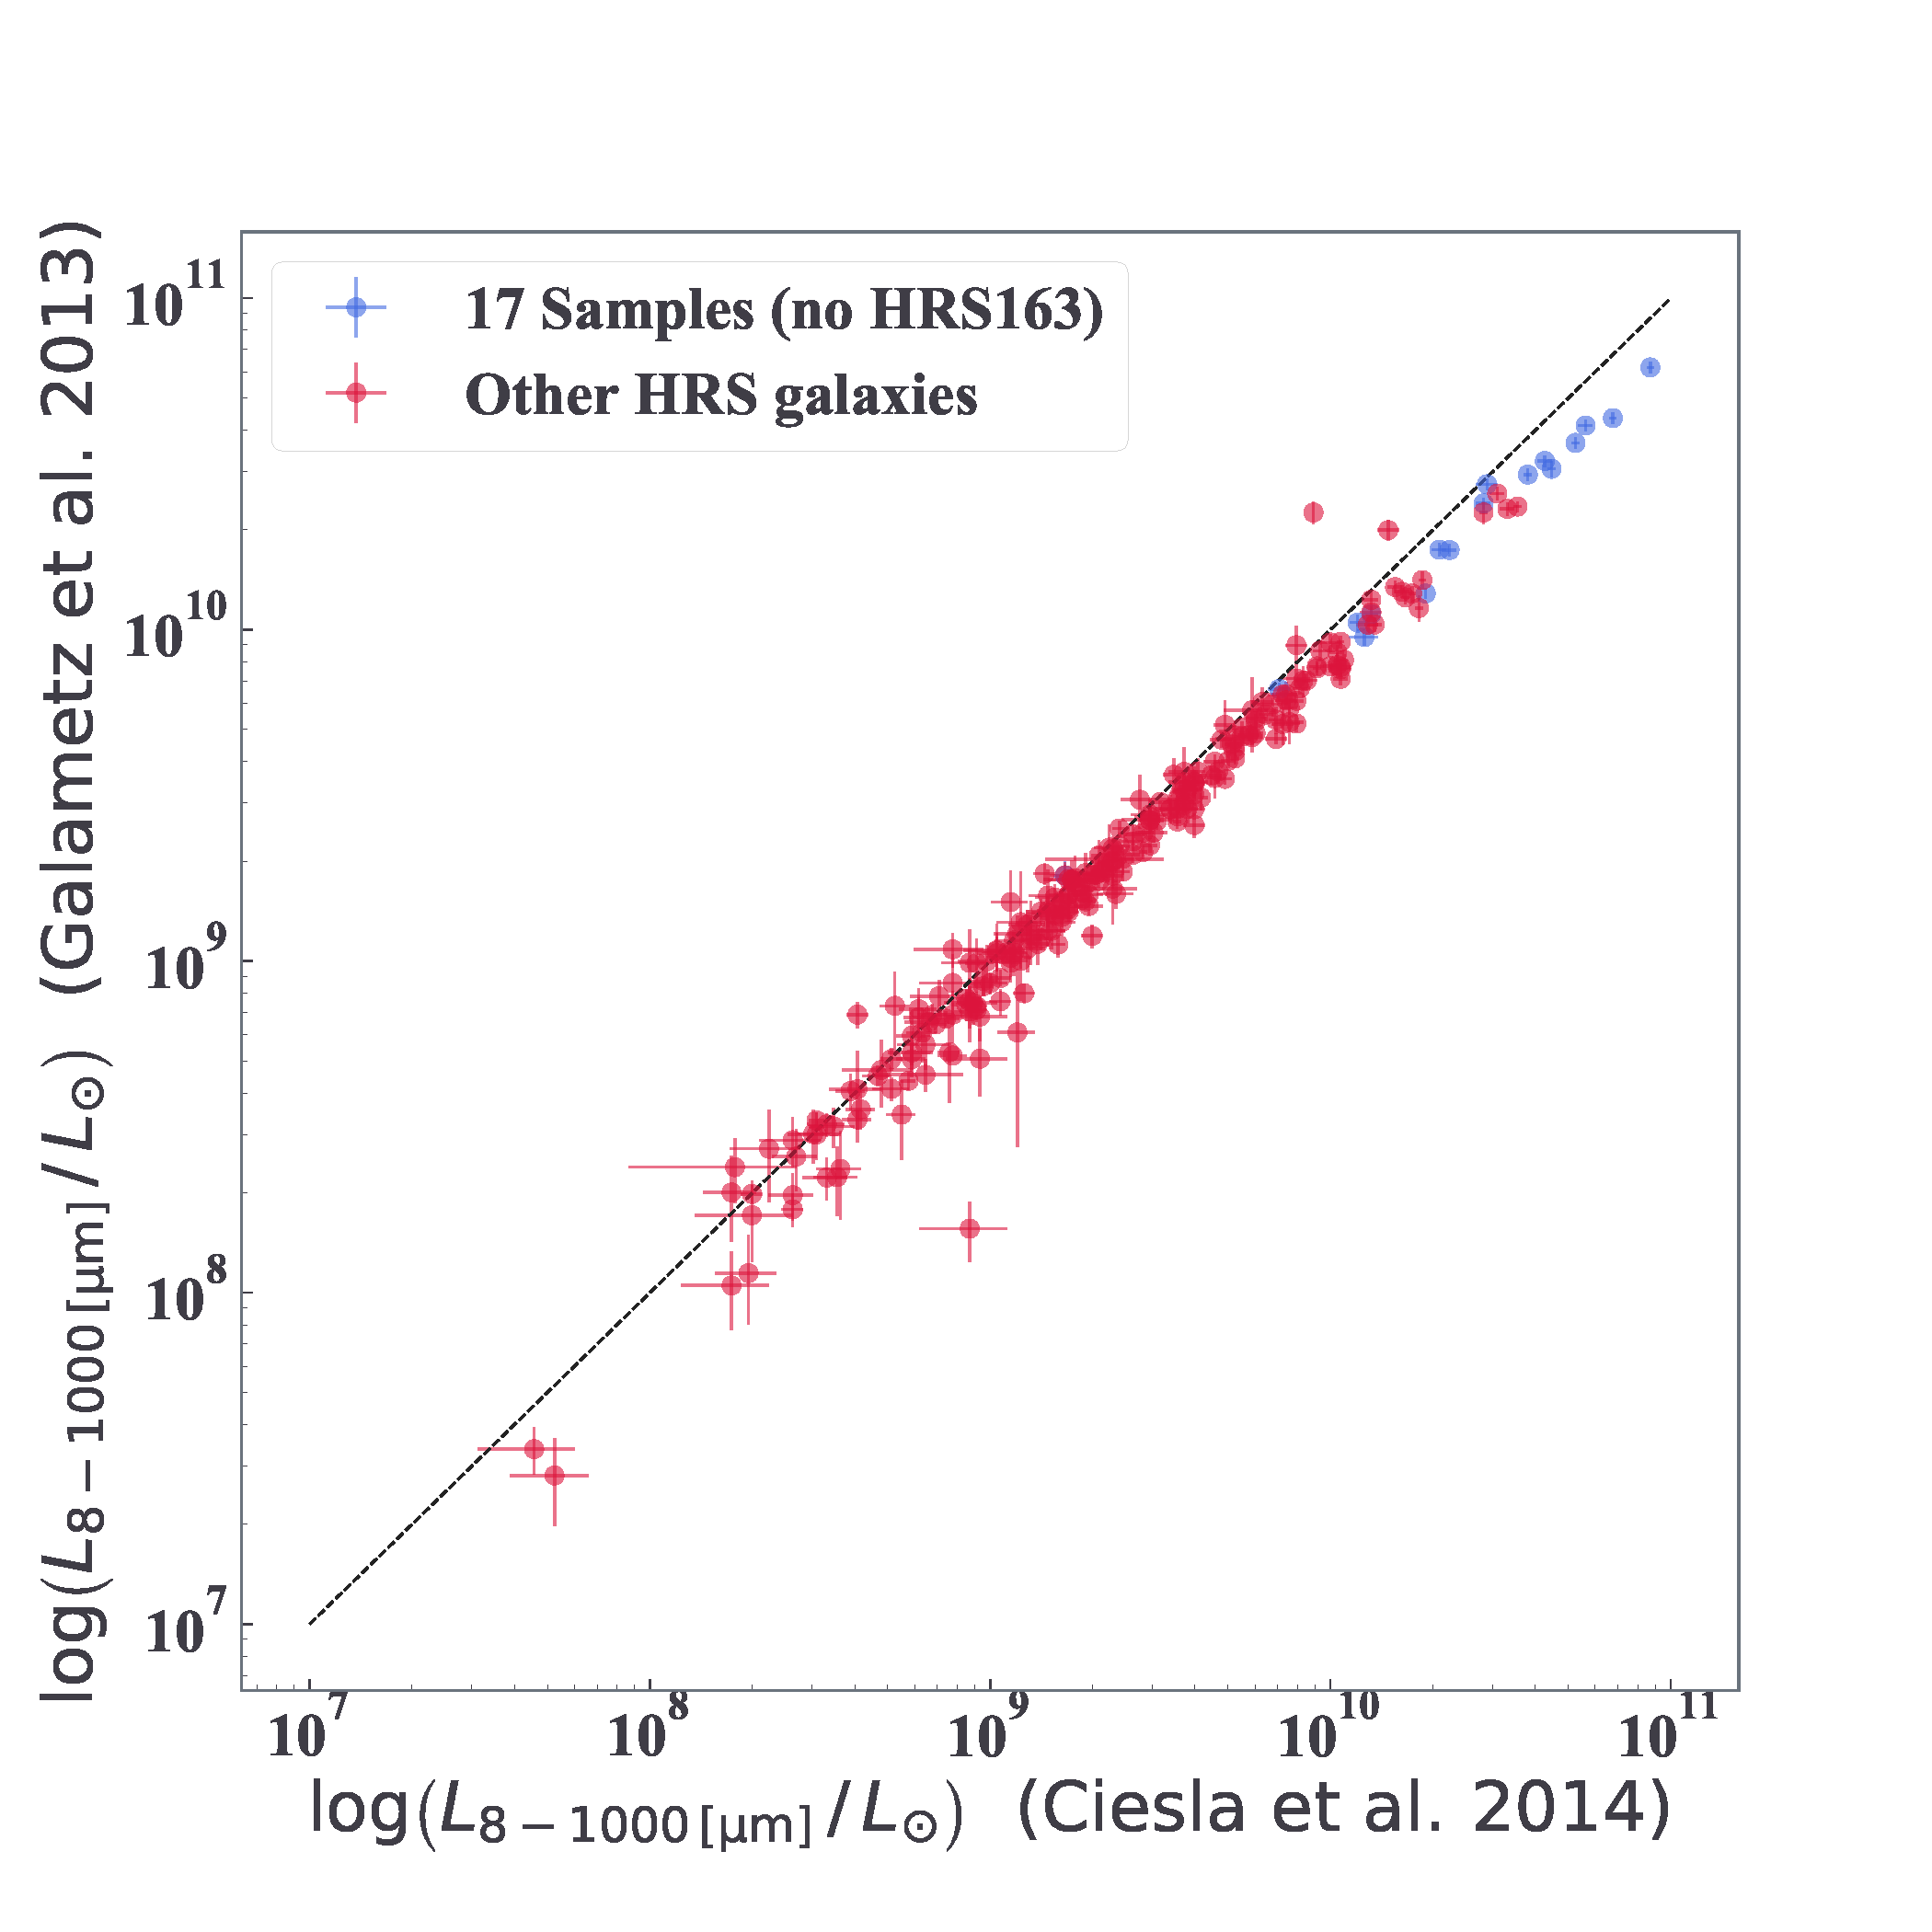
\includegraphics[width=.7\linewidth]{Chapter_4/Figures/Method_TIRcomparison.pdf}
    \caption[The comparison of total IR luminosities]{\label{fig:tircomparison}
        This figure shows the comparison of total IR luminosity at $8-1000\micron$ from different methods.
        Here, we show all HRS galaxies which have both luminosities.
        Blue plots show galaxy samples selected in Section~\ref{sec:crossmatching} and~\ref{sec:reducegalaxysamples}, and red ones show other HRS galaxies.
        The difference of both luminosities is less than factor 2.
    }
\end{figure}

Hereafter, we use $L_{8-1000\mathrm{\mu m}}$ obtained here to calculate the $q$ parameter and SFR\@.



\section{Fitting to $\qn$ parameters}\label{sec:fittingtoq}
Here, we show how to do the fitting to $\qn$.
%If I add the chapter 2, delete after , which emitted from~~~
At low frequencies around $100\MHz$, the synchrotron emission can be dominant, which emitted from high energy electrons accelerated by the supernova remnant.
In this paper, we assume radio emission has a single power-law on the frequency and adopt the following equation:

\begin{equation}\label{eq:q_fitting}
    q_{\nu} = -\gamma\log{\nu} + \beta
\end{equation}
where $q_{\nu}$ is defined by Equation~\ref{eq:q_def} at $\nu\MHz$, $\gamma$ is the power-law index showing the frequency dependence of $\qn$ and $\beta$ is the second fitting parameter.

In this study, we execute two types of fitting:

\begin{enumerate}
    \item Fitting to only MWA frequencies ($72-231\MHz$)
    \item Fitting to $1500\MHz$ besides MWA frequencies
\end{enumerate}

The flux data at $1500\MHz$ is obtained from \citet{Boselli2015}, and here we use only high-quality flux data (flag = 1).
These two types of fitting might allow us to judge the correctness of a single power-law assumption.
These fitting results are summarized in Section~\ref{sec:GammaDistribution}.



\section{Calculating the SFR}\label{sec:calculatingsfr}
In this section, I describe how to derive SFR from low-frequency radio emissions.\\
Here, we estimate the radio SFR, combining Equation~\ref{eq:q_def} with the following equations:

\begin{align}
    \mr{SFR}\msb{IR} &= 3.88 \times 10^{-44}\brp{\frac{L\msb{8-1000\,\mu m}}{\mr{erg}\,s^{-1}}}\label{eq:sfrir}\\
    q_{\nu\,\mr{MHz}} &= \q{1500\MHz} + \log{\brp{\frac{\nu\,\mr{MHz}}{1500\,\mr{MHz}}}}^{\gamma}\label{eq:q_nuto1500}
\end{align}

Equation~\ref{eq:sfrir} calculates SFR from the total IR emission in \citet{Murphy2011}, and Equation~\ref{eq:q_nuto1500} shows the difference of the $\qn$ between a certain wavelength $\nu$ and $1500\MHz$.

Substituting equation~\ref{eq:q_def} and~\ref{eq:q_nuto1500} into equation~\ref{eq:sfrir} yields the following equation to estimate SFR from radio emission at $\nu\MHz$:

\begin{equation}\label{eq:sfrfromradio}
    SFR_{\mr{Radio},\,\nu} = 1.46\times10^{-31}\times 10^{q\msb{1500\MHz}} {\brp{\frac{\nu\,\MHz}{1500\MHz}}}^{-\gamma} \times L_{\mr{Radio},\,\nu}
\end{equation}

In Section~\ref{sec:sfrfromlowradio}, I show the results of calculating SFR from the low-frequency radio using this equation and comparing it with the SFR from other indicator.



%\bibliographystyle{mnras}
%%\bibliography{example} % if your bibtex file is called example.bib
%\bibliography{masterthesis}

	\chapter{Results}\label{chap:results}
\begin{chapabstract}

In this chapter, we present our results with figures.
In Section~\ref{sec:GammaDistribution}, we show the $\qn$ frequency dependence for each galaxy with the distribution of $\gamma$.
In Section~\ref{sec:sfrfromlowradio}, we show the result of the comparison between the SFRs from thee radio emission and other indicators.

\end{chapabstract}


%\section{Final samples}
%
%Here, we will mention 18 samples and put the figure to compare it with CalistroRivera2017a.

\section{Distributions of $\gamma$}\label{sec:GammaDistribution}

\begin{figure}[htbp]
	\centering
	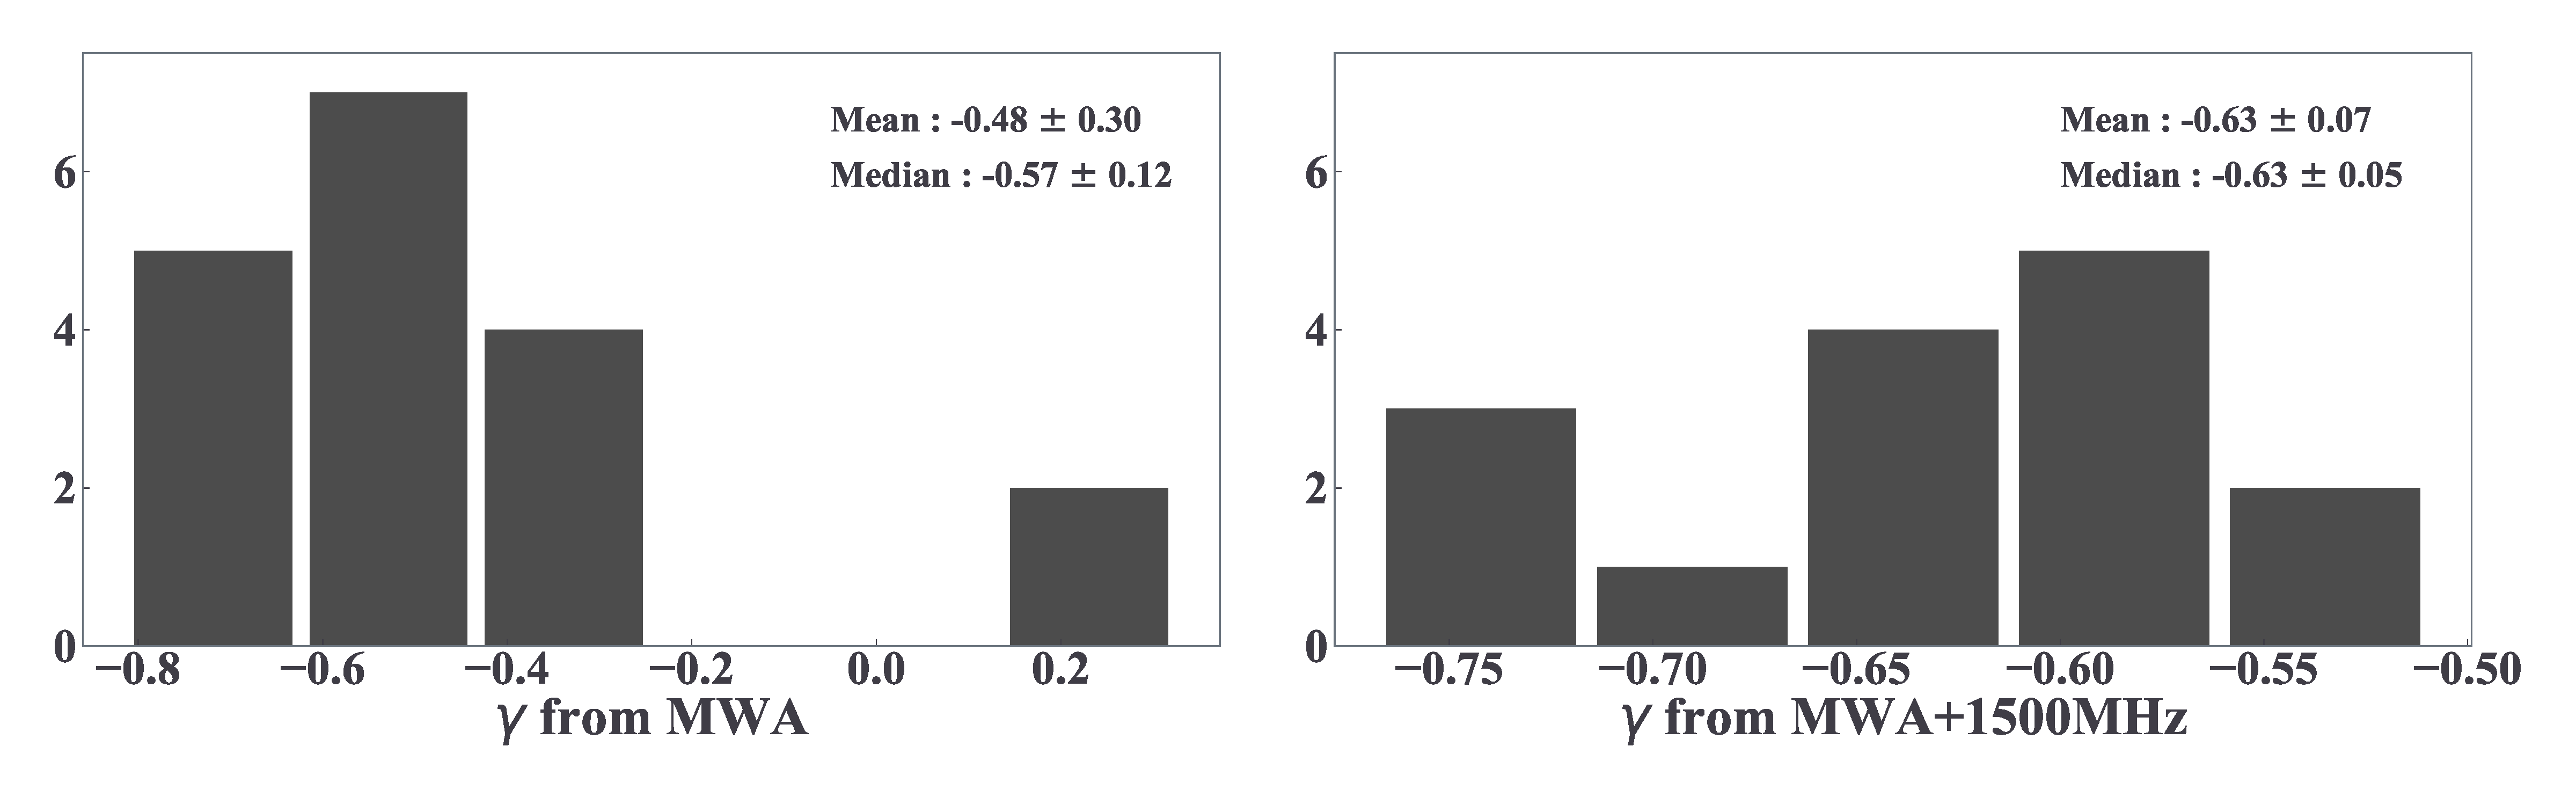
\includegraphics[width=\linewidth]{Chapter_5/Figures/Result_comparehist.pdf}
    \caption[Histograms of $\gamma$ from the fitting]{\label{fig:comparehist}
        The distributions of $\gamma$ for each fitting.
        The left figure indicates the fitting result with only MWA frequencies, and the right one does with 1500 [MHz] besides MWA frequencies.
    }
\end{figure}

\begin{figure}[htbp]
	\centering
	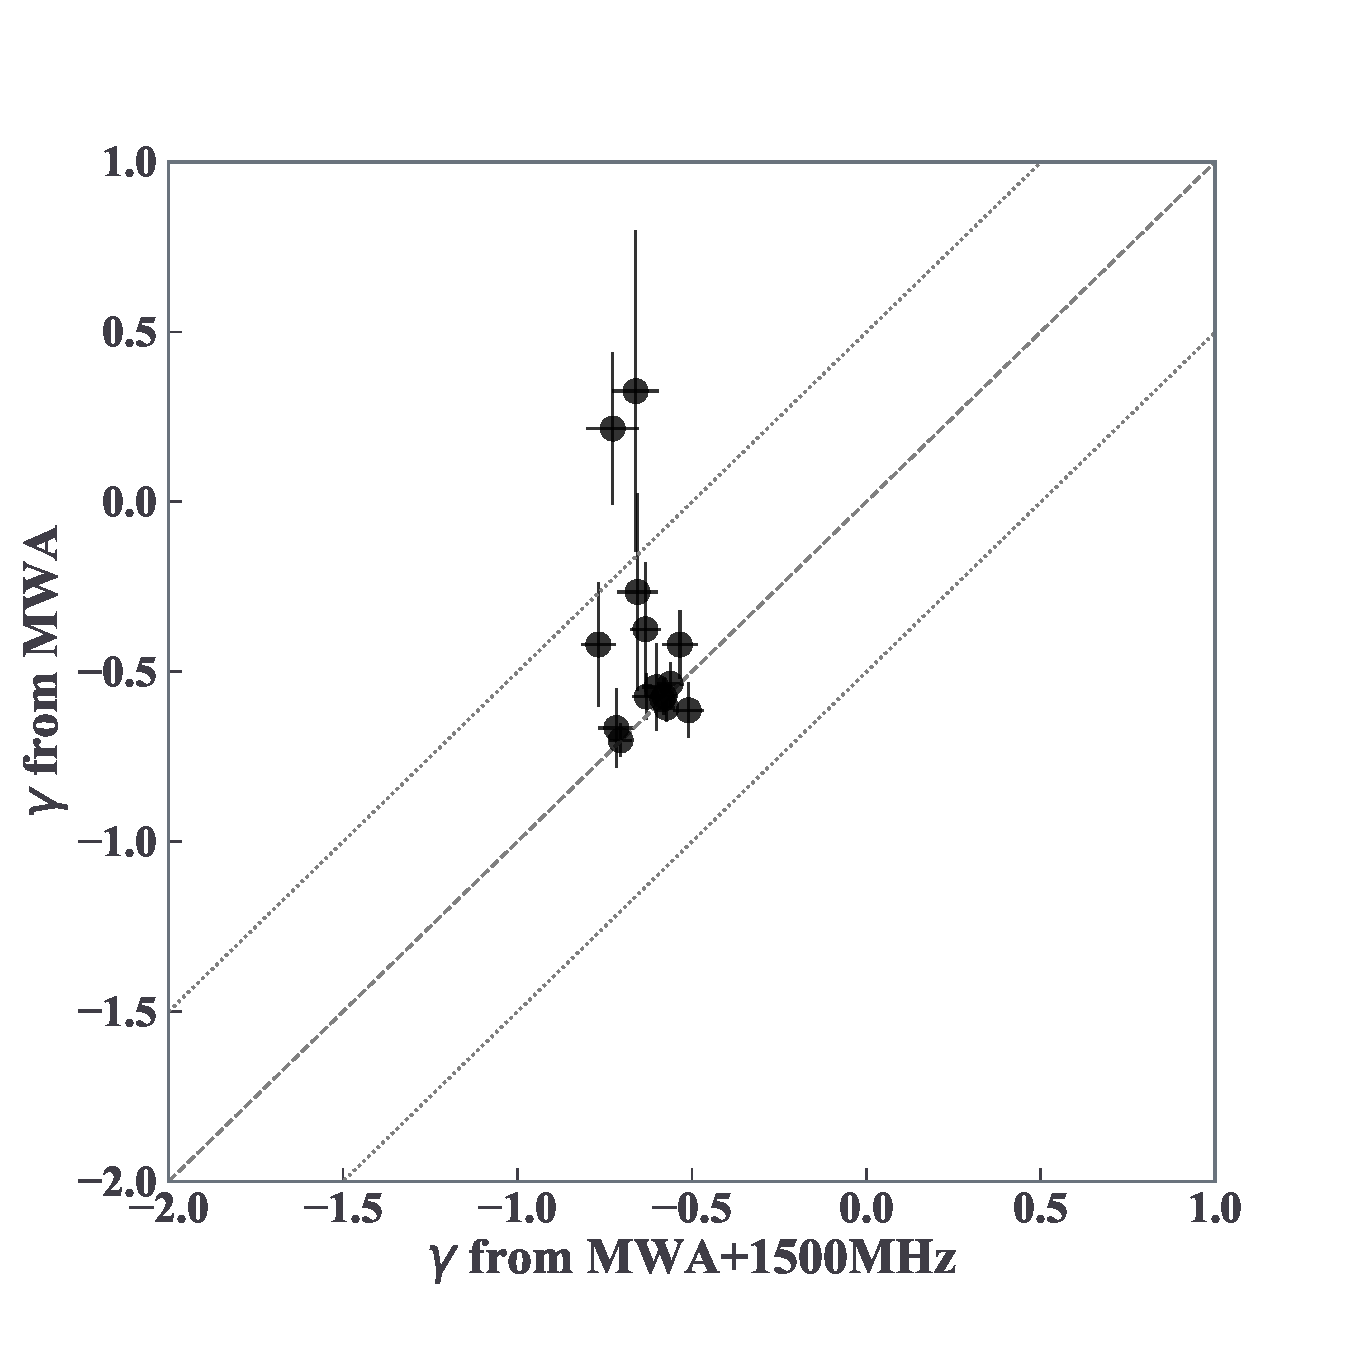
\includegraphics[width=.6\linewidth]{Chapter_5/Figures/Result_comparealpha.pdf}
    \caption[The comparison of $\gamma$ from different fitting methods]{\label{fig:comparegamma}
        The difference of $\gamma$ for each fitting method.
        The solid line shows the one to one correlation, and dotted lines show 0.5 dex away from the solid line.
        Each plot shows each galaxy.
        In this figure, we can see $\gamma$ fitted to only MWA frequencies are relatively flatter.
    }
\end{figure}

Here, we show two kinds of fitting results.
The left plot in Figure~\ref{fig:comparehist} is the $\gamma$ distribution from the fitting only to MWA frequencies, and the right one is to $1500\MHz$ besides MWA frequencies.
We show the mean and median with the standard and quantile deviation in both plots.
Since we adopt high-quality flux data at $1500\MHz$ \citep{Boselli2015}, three samples (HRS 122, 163 and 204) are fitted only in the case with MWA fluxes.
Figure~\ref{fig:comparegamma} compares $\gamma$ from different fitting fluxes for each galaxy.

In these figures, we can find that there are two galaxies (HRS 25 and 144) with a relatively flatter $\gamma$ fitted only to MWA frequencies.
This result suggests that there is a critical frequency where the turnover arises between MWA frequencies and $1500\MHz$.
At low frequencies, the spectral is prone to be flatter due to the free-free absorption \citep[e.g.,][]{CalistroRivera2017a, Schober2017, Chyzy2018}.
In addition to this, \citet{Schober2017} show that a Milky Way like galaxy (similar SFR) has the critical frequency order of magnitude lower than the MWA frequency.
However, HRS 25 and 144 have a Milky Way like SFR \citep{Boselli2015} and a critical frequency between MWA frequencies and $1500\MHz$.
This result cannot be explained by \citet{Schober2017}.
One possible explanation is that fewer number of fluxes yields less constraint of the fitting and the flatter $\gamma$ for HRS 25 and the galactic nuclei affects the spectral for HRS 144 identified as a Seyfert galaxy from the BPT diagram \citep[e.g.,][]{Baldwin1981, Kewley2001, Kauffmann2003, Schawinski2007}.
The BPT diagram demonstrates to identify LINER, Seyfert galaxies from the normal star-forming ones using optical line emissions.
For understanding these galaxies, we would need the case study with more data in a wide frequency range.

If we neglect these galaxies, the mean $\gamma$ changes from $-0.48\pm0.30$ to $-0.57\pm0.14$ for the fitting without $1500\MHz$ case and from $-0.63\pm0.08$ to $-0.62\pm0.08$ with $1500\MHz$ case.
The mean $\gamma$ does not vary in the case with $1500\MHz$.
This result means that HRS 25 and 144 do not affect the fitting result among MWA frequencies and $1500\MHz$, although they do the mean $\gamma$ from the fitting only to MWA frequencies.
Therefore, in this paper, we adopt the averaged $\gamma$ obtained from the fitting across the MWA frequency to $1500\MHz$ for calculating SFR (Section~\ref{sec:sfrfromlowradio}).\\
The fitting results of 18 galaxy samples are shown in Appendix~\ref{chap:fittingresults}.



\section{Comparing SFR Indicators}\label{sec:sfrfromlowradio}

\begin{figure}[htbp]
	\centering
	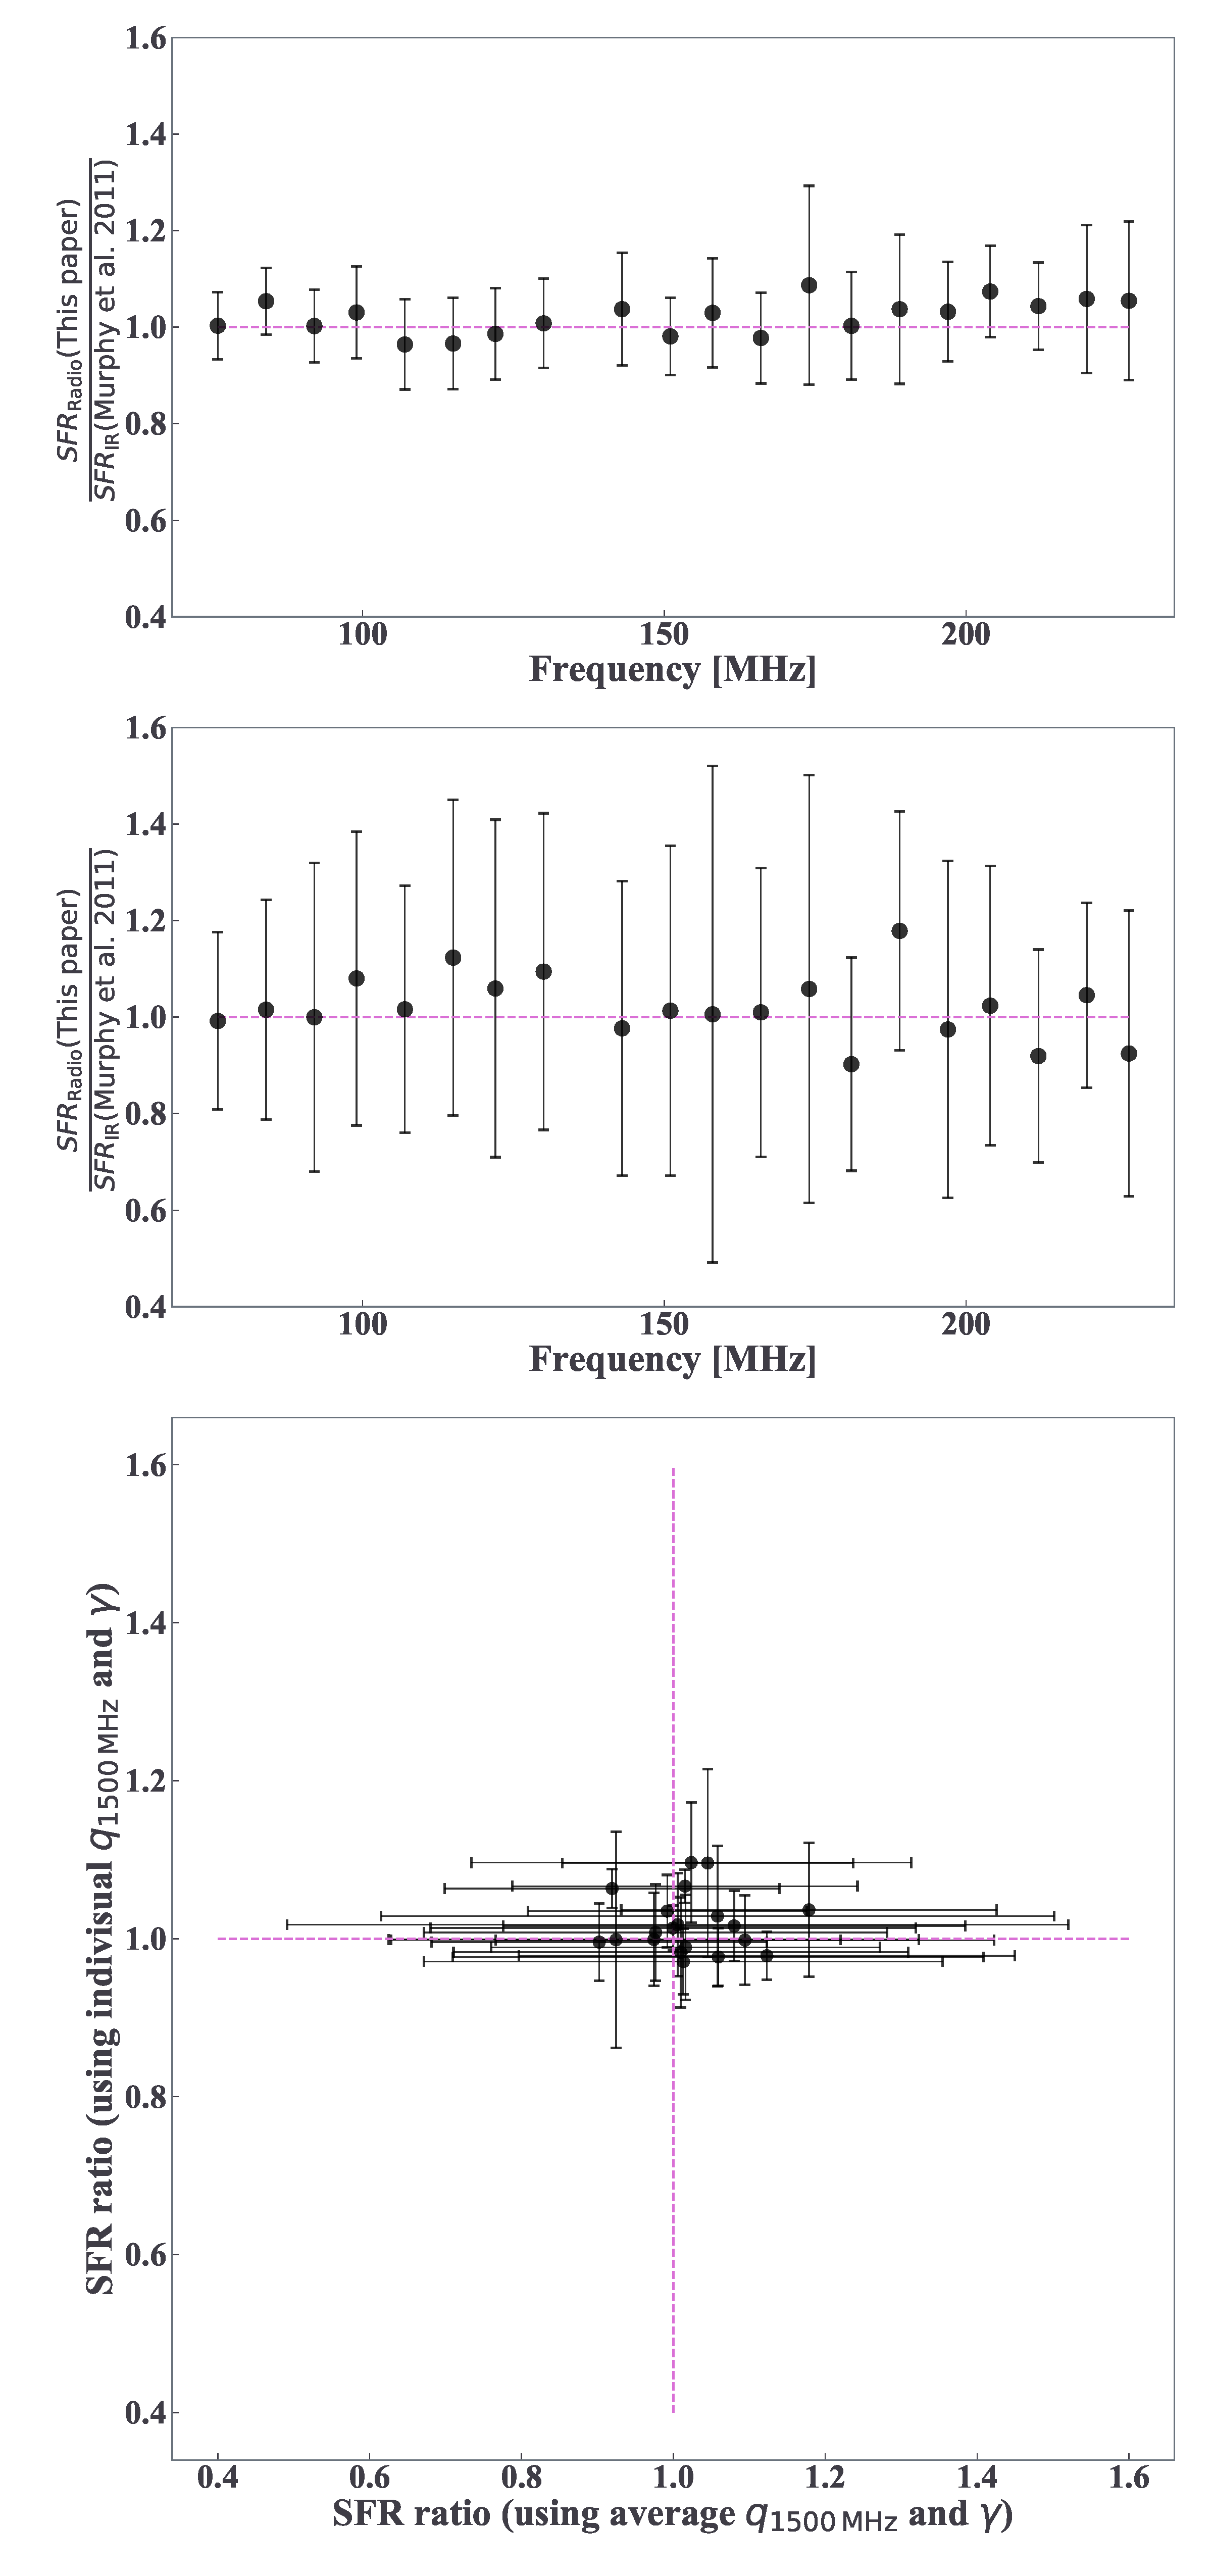
\includegraphics[width=.6\linewidth]{Chapter_5/Figures/Result_sfrratio.pdf}
    \caption[The consistency of the radio SFR]{\label{fig:sfrratio}
        The SFR ratio between $\mr{SFR}_{\mr{Radio},\,\nu}$ and $\mr{SFR}\msb{IR}$ at each MWA frequency.
        The difference between the upper and middle plots is the calibration parameters to calculate $\mr{SFR}_{\mr{Radio},\,\nu}$.
        Individual or averaged $\gamma$ and $\q{1500\MHz}$ are used for the upper or middle plots, respectively.
    The bottom plot compares SFR ratios calculated with different calibrations.
    }
\end{figure}

\begin{figure}[htbp]
	\centering
	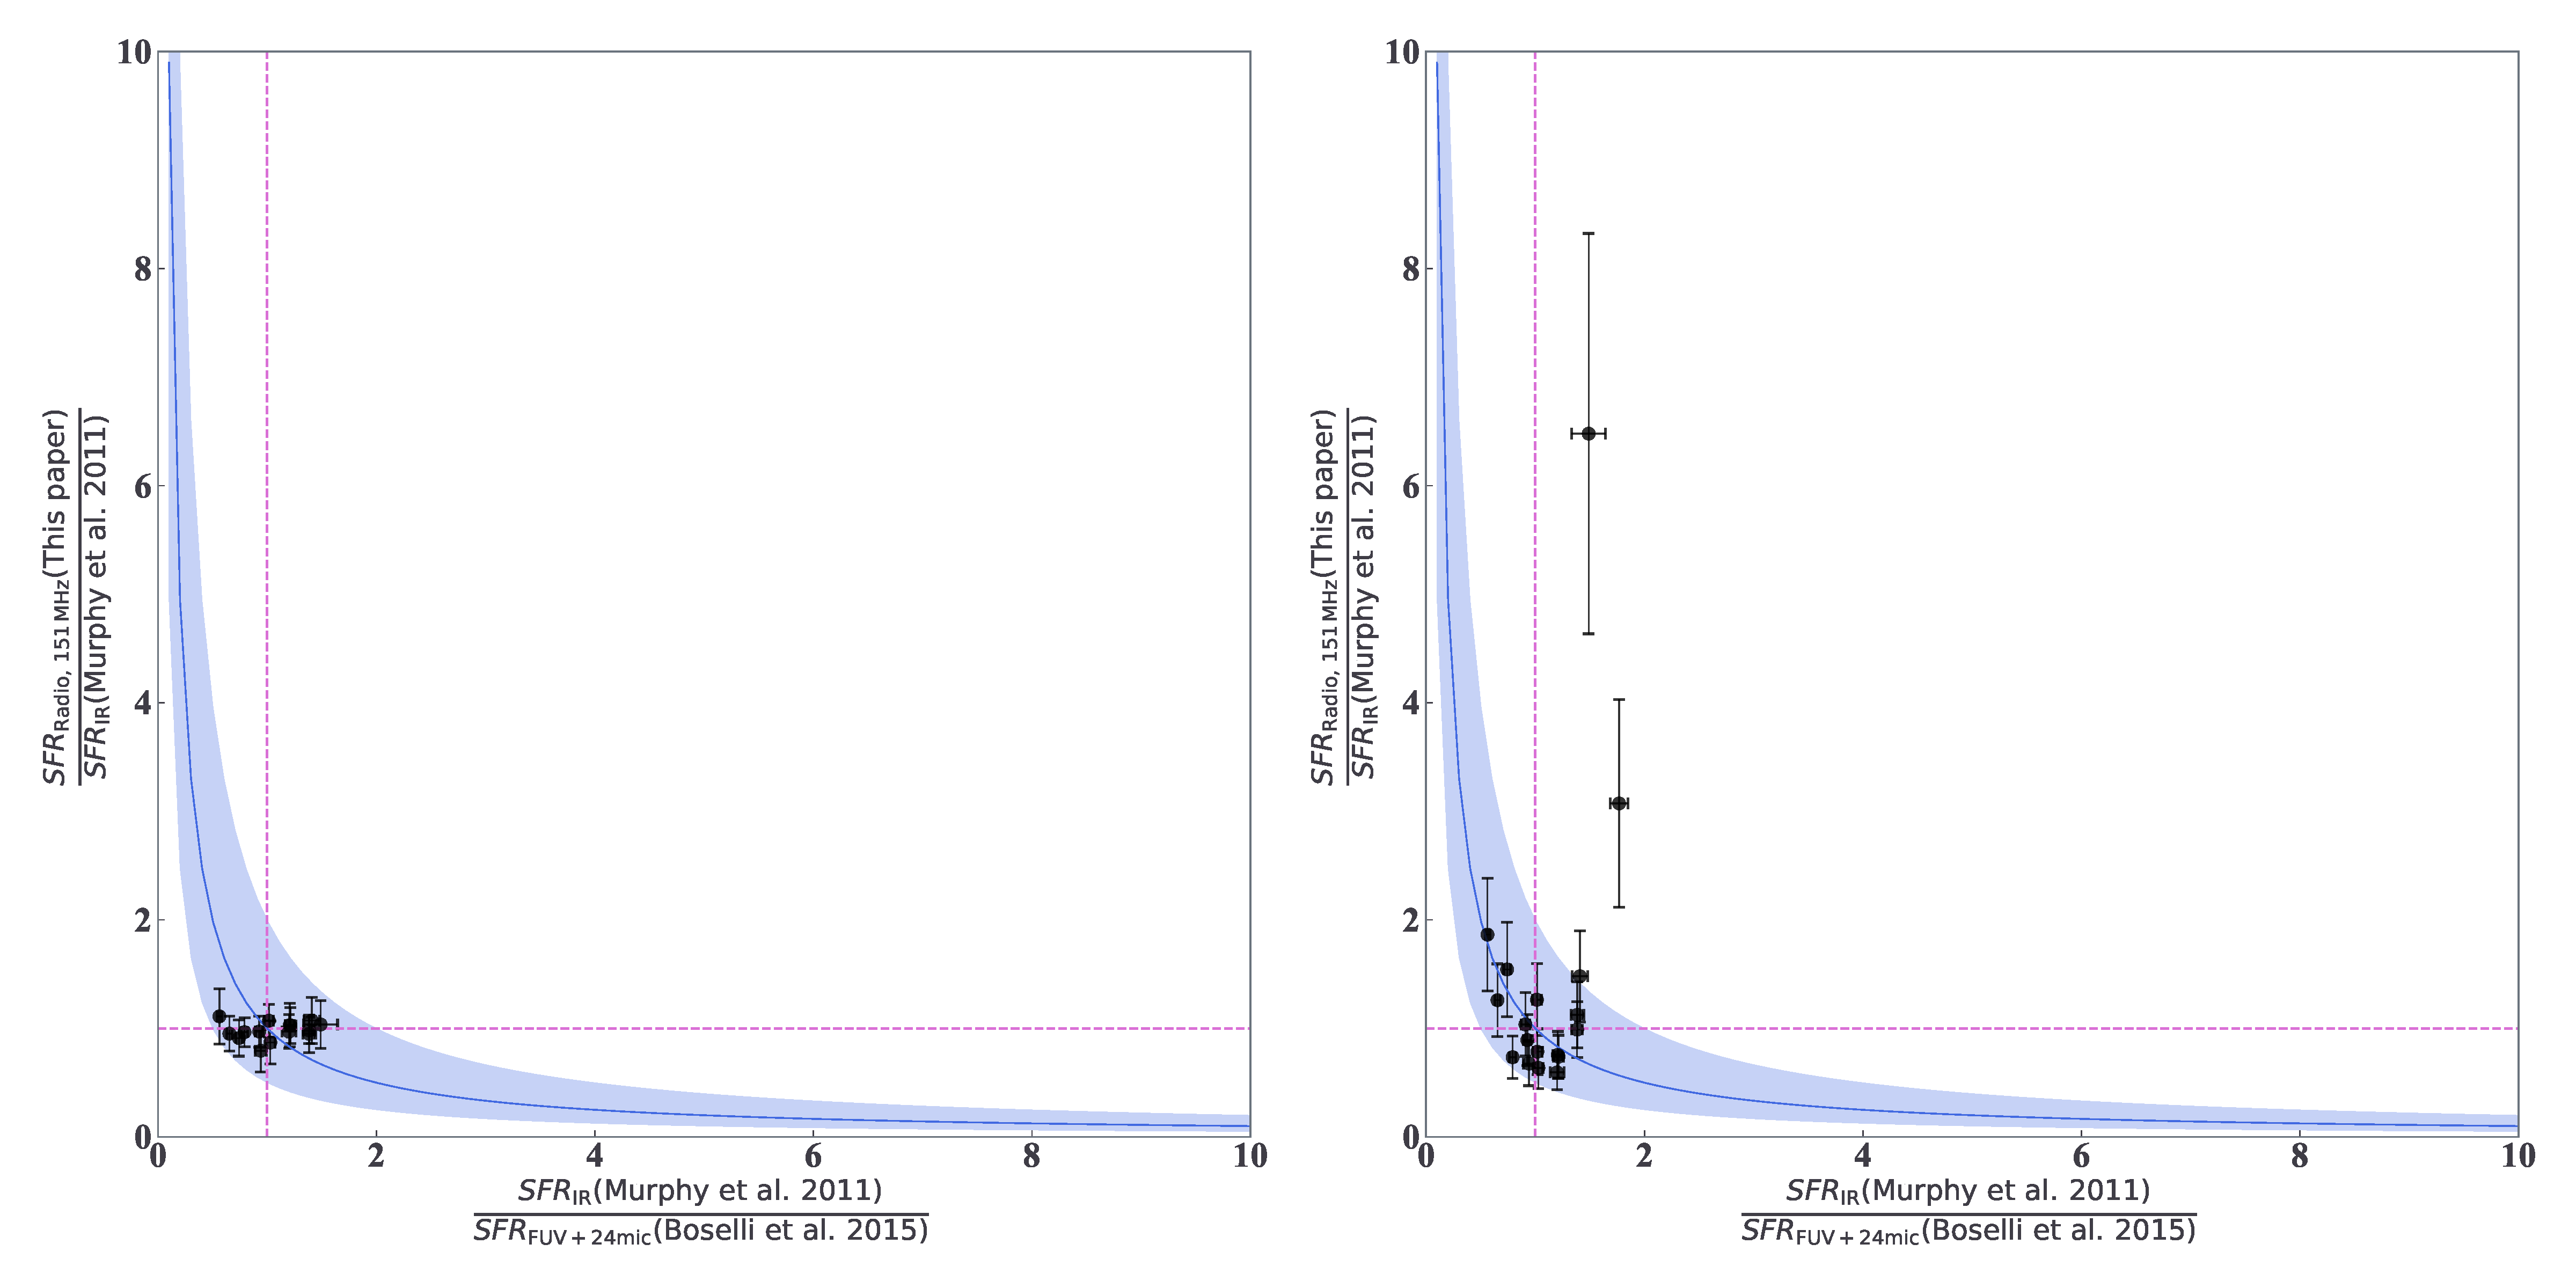
\includegraphics[width=\linewidth]{Chapter_5/Figures/Result_sfrratios.pdf}
    \caption[The consistency of the radio SFR with $\mr{SFR}\msb{IR}$ and $\mr{SFR}\msb{FUV+24\,\micron}$]{\label{fig:sfrratios}
        The SFR ratios from different indicators.
        The vertical and horizontal axes are $\mr{SFR}\msb{Radio,\,151\MHz}\ /\ \mr{SFR}\msb{IR}$ and $\mr{SFR}\msb{IR}\ /\ \mr{SFR}\msb{FUV+24\,\micron}$ in both plots.
        Magenta dashed lines indicate the unity for each SFR ratio, and the solid blue lines do for the SFR ratio between $\mr{SFR}\msb{Radio,\,151\MHz}\ /\ \mr{SFR}\msb{FUV+24\,\micron}$.
        The blue shaded region shows the ratio between $\mr{SFR}_{\mr{Radio},\,151\MHz}$ and $\mr{SFR}\msb{FUV+24\,\micron}$ within factor two ($0.5 \leq \mr{SFR}_{\mr{Radio},\,151\MHz}\ /\ \mr{SFR}\msb{FUV+24mic} \leq 2$).
        The difference between the upper and middle plots is the calibration parameters to calculate $\mr{SFR}_{\mr{Radio},\,151\MHz}$.
    }
\end{figure}

Here, we show the result from comparing $\mr{SFR}_{\mr{Radio},\,\nu}$ defined by Equation~\ref{eq:sfrfromradio} with $\mr{SFR}\msb{IR}$ (Equation~\ref{eq:sfrir}) and $\mr{SFR}\msb{FUV+24mic}$ \citep{Boselli2015}.

Figure~\ref{fig:sfrratio} shows the SFR ratio between $\mr{SFR}_{\mr{Radio},\,\nu}$ and $\mr{SFR}\msb{IR}$.
For drawing the upper figure, we substitute the individual $q_{1500\MHz}$ and $\gamma$ into Equation~\ref{eq:sfrfromradio}.
We calculate $\mr{SFR}_{\mr{Radio},\,\nu}$ at each MWA frequency, and plot the mean value.
Note that the number of galaxies taken for the mean at each frequency is different because we use only high-quality fluxes and some of them are dropped.
In this case, we can see it is consistent with $\mr{SFR}\msb{IR}$ within a 20\% error.
For the middle figure, we substitute the averaged $q_{1500\MHz}$ and $\gamma$ instead of individual values.
This calibration method yields larger scatters compared to the previous one.
However, $\mr{SFR}_{\mr{Radio},\,\nu}$ is still consistent with $\mr{SFR}\msb{IR}$.
The bottom figure shows the SFR ratio comparison from different calibrations.
In this figure, it is clear that SFR calculated from the averaged value has more significant scatters than from the individual parameters.

These figures give us the idea that calculating radio SFR needs the spectral energy distribution for less uncertainty.
For the spectral, we find that the single power-law assumption yields the radio SFR with the consistency within 20\%, even including galaxies that might have a flatter spectral at low frequencies.

Figure~\ref{fig:sfrratios} shows the comparison of SFR ratios.
For both plots in the figure, vertical and horizontal axes show the ratio between $\mr{SFR}_{\mr{Radio},\,151\MHz}$ and $\mr{SFR}\msb{IR}$, between $\mr{SFR}\msb{IR}$ and $\mr{SFR}\msb{FUV+24mic}$, respectively.
Since the frequency at $151\MHz$ is the only flux band that all our samples have high-quality data, we use the radio emission at the band.
Here, we check the consistency of the radio SFR with other SFR indicators.
While $\mr{SFR}\msb{IR}$ traces the only dust emission, $\mr{SFR}\msb{FUV+24mic}$ does the direct young massive stellar emission dust-corrected by the IR radiation at $24\,\micron$ \citep{Murphy2011, Kennicutt2012}.
This figure shows how consistent the radio SFR is with this direct emission tracer.
The difference between these plots is the calibration parameter for calculating $\mr{SFR}_{\mr{Radio},\,151\MHz}$.
The individual $q_{1500\MHz}$ and $\gamma$ are used for the left plot and the averaged ones for the right plot.
The blue shaded region shows the ratio between $\mr{SFR}_{\mr{Radio},\,151\MHz}$ and $\mr{SFR}\msb{FUV+24\,\micron}$ within factor two ($0.5 \leq \mr{SFR}_{\mr{Radio},\,151\MHz}\ /\ \mr{SFR}\msb{FUV+24\,\micron} \leq 2$).
In the figure, we can see that the radio SFR using individual parameters is also consistent with $\mr{SFR}\msb{FUV+24\,\micron}$ within the factor of 2.
However, in the other case, there are two galaxies (HRS 306 and 144) whose radio SFR overestimates.
This is because these galaxies have stronger radio emission (lower $\qn$) than the extrapolated average value at $151\MHz$.



%\bibliographystyle{mnras}
%%\bibliography{example} % if your bibtex file is called example.bib
%\bibliography{masterthesis}

	\chapter{Discussions}\label{chap:discussions}
\begin{chapabstract}

In this Chapter, we show further discussion on our results in Chapter~\ref{chap:results}.
Section~\ref{sec:comparingthecalibration} compares our fitting results, mainly the frequency dependence of $\qn$ with previous studies.
Section~\ref{sec:radiosfruncertainty} shows the comparison of the radio SFR calibration with \citet{CalistroRivera2017a}.
Section~\ref{sec:galaxypropertiesfortheradiosfr} describes how galaxy properties affect the SFR estimation.
Here, we focus on the active galactic nuclei in a galaxy and the \nh-deficiency.
Section~\ref{sec:nondetectedgalaxiesbythegleamsurvey} describes HRS galaxies whose radio counterparts are not detected by the GLEAM survey.
In this Section, we also mention the possibility of their radio source detection by the updated GLEAM survey.

\end{chapabstract}

\section{Comparing the Calibration with Previous Results}\label{sec:comparingthecalibration}

Here, we compare our results in Section~\ref{sec:GammaDistribution} with previous research.
From our samples, we obtain the mean $\gamma=-0.63 \pm 0.07$ from the fitting between MWA frequencies and $1500\MHz$.
\citet{CalistroRivera2017a} and \citet{Chyzy2018} obtained $-0.78 \pm 0.24$ and $-0.56 \pm 0.11$, respectively.

\begin{figure}[htbp]
	\centering
	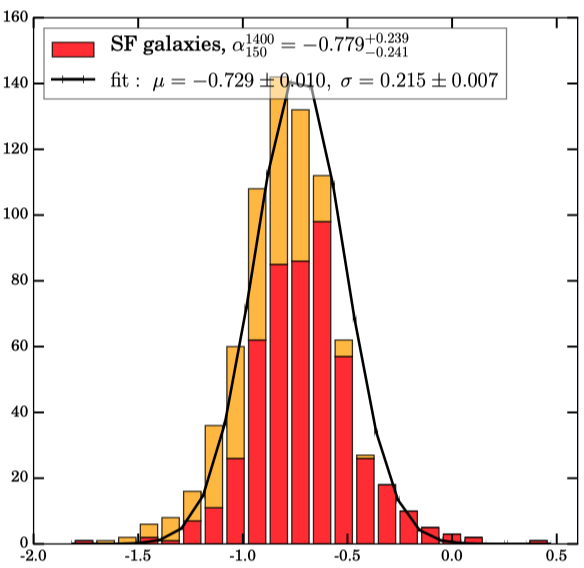
\includegraphics[width=.7\linewidth]{Chapter_6/Figures/CalistroRivera2017_Figure7.png}
    \caption[The histogram of the spectral index in \citet{CalistroRivera2017a}]{\label{fig:CalistroRivera2017_figure7}
        The histogram of the spectral index corresponding to $\gamma$ in this study.
        They calculate it between $150\MHz$ (LOFAR;~\citealt{Williams2016}) and $1.4\GHz$ (Westerbork Synthesis Radio Telescope, WSRT;~\citealt{DeVries2002}).
        Red and orange histograms show the samples detected and non-detected by WSRT\@.
        To estimate the flux of non-detected samples, they extract aperture fluxes from the source location known by LOFAR on the radio map (forced photometry technique).
        The black solid line displays the Gaussian fitting function.
        They put the average $\mu$ and standard deviation $\sigma$ from the fitting on the upper right in the figure
        (Adapted from \citealt{CalistroRivera2017a}).
    }
\end{figure}

\begin{figure}[htbp]
	\centering
	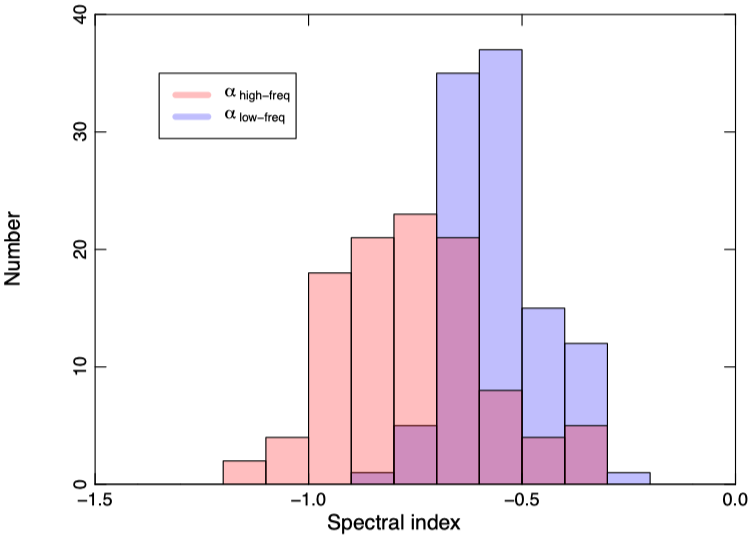
\includegraphics[width=.8\linewidth]{Chapter_6/Figures/Chyzy2018_Figure4.png}
    \caption[The histogram of the spectral index in \citet{Chyzy2018}]{\label{fig:Chyzy2018_figure4}
        Red and blue histograms show the spectral index corresponding to $\gamma$ in this study calculated fluxes from $1.3\GHz$ to $5\GHz$ and $150\MHz$ to $1.4\GHz$, respectively.
        They show histogram in violet where they are overlapping.
        From the definition, we should compare our result with the blue one.
        They calculate it between $150\MHz$ (The Multifrequency Snapshot Sky Survey, MSSS;~\citealt{Heald2015}) and $1.4\GHz$ (the NRAO VLA Sky Survey, NVSS;~\citealt{Condon1998})
        (Adapted from \citealt{Chyzy2018}).
    }
\end{figure}

The difference of these might result from the selection of galaxy samples.
While we use nearby galaxies within $25\,\mr{Mpc}$, \citet{CalistroRivera2017a} do 758 galaxies up to $z\sim2$, and \citet{Chyzy2018} do 118 galaxies up to $z=0.04$.

\citet{Chyzy2018} indicate that the slope is steeper at higher frequencies ($1.3 \sim 5\GHz$), and this might steepen the slope of galaxy samples in \citet{CalistroRivera2017a} which adopt galaxies up to $z\sim2$.
Since \citet{CalistroRivera2017a} did not execute $k$-correction for Figure~\ref{fig:CalistroRivera2017_figure7}, some $\alpha$ values indicate the spectral index at higher frequencies, which might be expected to have a steeper slope.
Considering the value and scatter, our result using the Herschel reference sample would be consistent with previous findings.
Indeed, the frequency dependence of the low-frequency emission and its relation with IR emission is still uncertain.



\section{Uncertainty of Radio SFR}\label{sec:radiosfruncertainty}

In Section~\ref{sec:sfrfromlowradio}, we show the consistency of our SFR calibrations using the low-frequency emission.
For calculating the more accurate radio SFR, we need its spectral energy distribution for each galaxy, as we have already shown in Section~\ref{sec:sfrfromlowradio}.
Since star-forming galaxies have a wide variety of $\qn$ at low frequencies ($\sim 0.53\,\mr{dex}$ in Figure~14, 15; \citealt{CalistroRivera2017a}) and still we do not know the physical details, the radio SFR calibration has considerable uncertainty.
Substituting averaged $\gamma$ and $\q{1500\MHz}$ obtained from our sample galaxies into Equation~\ref{eq:sfrfromradio} yields the following equation:

\begin{equation}\label{eq:sfrradio_calibration}
    \mr{SFR}_{\mr{Radio},\,150\MHz} = \brp{1.03\pm0.27} \times 10^{-29} \times \brp{\frac{L_{\mr{Radio},\,150\MHz}}{\mr{erg}\,\mr{s}^{-1}}}
\end{equation}
where we substitute the median values of $\gamma=-0.63$, $\q{1500\MHz}=2.48$ from our samples and $\nu=150\MHz$ into Equation~\ref{eq:sfrfromradio}.

\citet{CalistroRivera2017a} have obtained the coefficient of $0.76 \pm 0.08$ in Equation~\ref{eq:sfrradio_calibration} for nearby galaxies ($z = 0$) from their calibration.

We should keep our mind that the SFR calibration has non-negligible uncertainty, possibly caused by the galaxy selection and the variety of $\qn$ at low frequencies.
For estimating SFR accurately, we need the radio spectral with multi-band observation.



\section{Galaxy Properties for the Radio SFR}\label{sec:galaxypropertiesfortheradiosfr}

In this Section, we discuss how the galaxy property affect the results mentioned in previous Sections.
Here, we focus on the central engine and the environment of a galaxy.
The central engine in a galaxy driven by the supermassive black hole and the baryon accretion is called active galactic nuclei and known as another radio source.
Although we have eliminated galaxies which have strong radio emission against their star formation activity in Section~\ref{sec:reducegalaxysamples}, there are still some galaxies in our sample, which might have an active galactic nuclei identified by the optical line emissions.
These kinds of galaxies that might have a strong radio emission are called Seyfert or LINER galaxies.
And they possibly affect our results due to their radio emissions irrelevant to the star-formation activity.
Here, we investigate this property using the BPT diagram mentioned in Section~\ref{sec:GammaDistribution} and find three galaxies (HRS 144, 163 and 220) in our sample that have sharp optical emission lines (Figure~\ref{fig:bpt_diagram}).
In the BPT diagram, HRS 144 and 163 are found to be Seyfert galaxies, and HRS 220 is LINER galaxy.

\begin{figure}[htbp]
	\centering
	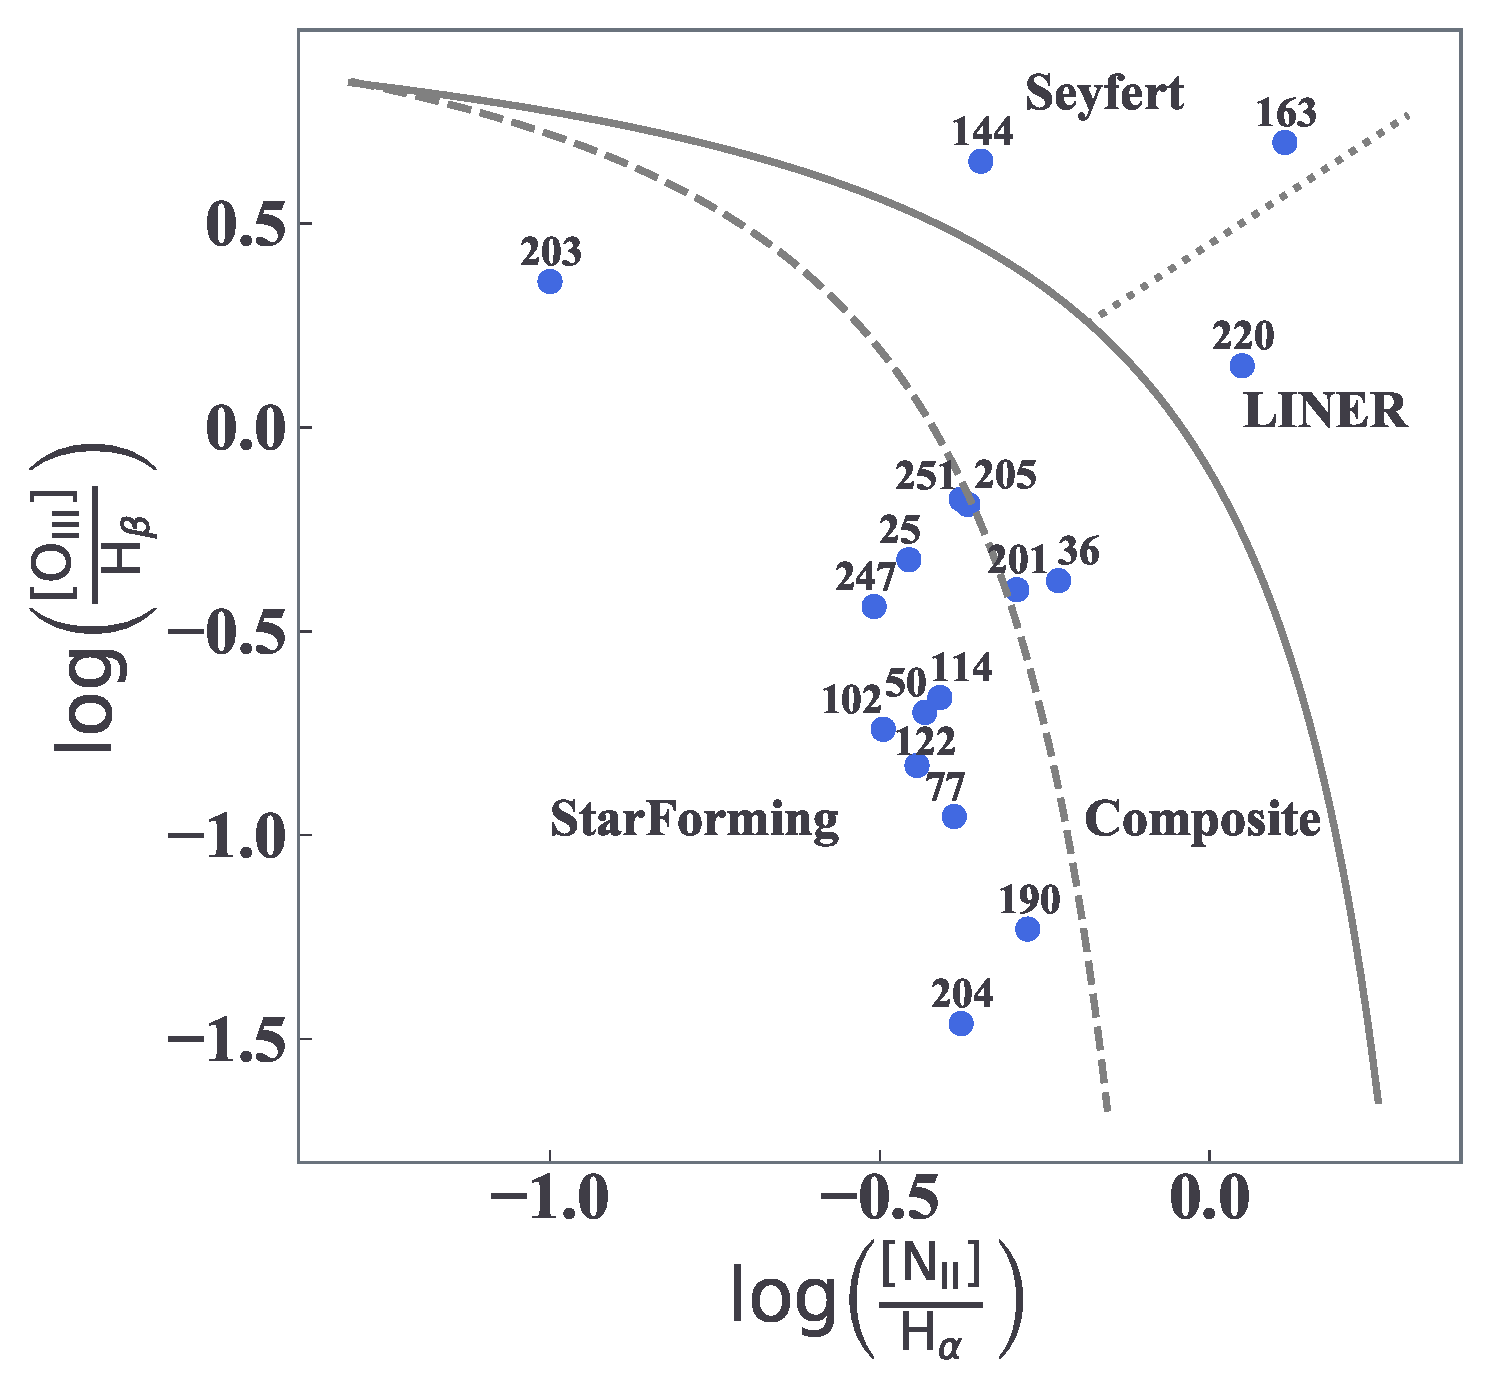
\includegraphics[width=.7\linewidth]{Chapter_6/Figures/Discuss_bpt.pdf}
    \caption[BPT diagram for 18 galaxy samples]{\label{fig:bpt_diagram}
        The BPT diagram is for 18 galaxy samples.
        Since HRS 306 does not have any line emission data, we do not plot it on the plot.
        The solid, dashed and dotted lines show the borders of different kinds of nuclei.
        We draw these lines based on \citet{Kewley2001, Kauffmann2003, Schawinski2007}, respectively.
    }
\end{figure}

After that, we also examine the galaxy environment of each galaxy.
\citet{Boselli2014} have already calculated the \nh-deficiency (\nh-def) for all HRS galaxies.
\nh-deficient galaxy is defined as a galaxy whose the \nh~mass is much smaller than the expected one based on the morphology and the size of a galaxy \citep{Haynes1984, Boselli2009}.

The definition of \nh-deficiency is as follows:

\begin{equation}\label{eq:definitionofHIdeficiency}
    \text{\nh-def} = \log\brp{M\msb{\nh,\,expected}} - \log\brp{M\msb{\nh,\,observed}}
\end{equation}
where $\log\brp{M\msb{\nh,\,expected}}$ is defined by \citet{Haynes1984}:

\begin{equation}\label{eq:definitionofexpectedHIdef}
    \log\brp{h^2 M\msb{\nh,\,expected}} = c + d\log\brp{h\times\mr{diam}}^2
\end{equation}
where $c$ and $d$ are weak functions of the galaxy morphology, $\mr{diam}$ is the linear diameter of the galaxy and $h=H_0 / 100$.

Here, we regard a galaxy whose \nh-deficiency is more than 0.4 as a \nh-deficient galaxy and the other case as a normal galaxy, which is the same criteria in \citet{Ciesla2016}.
\nh-deficiency is known to represent not only the amount of the \nh~mass but also a galaxy environment.
This is because \nh-deficiency might be attributed to the tidal stripping or ram pressure, which happens in the dense region (e.g., the center of a cluster).
Therefore, we can roughly assume that \nh-deficient galaxies are located in the dense regions, and normal galaxies are the field galaxies.
The relation between a galaxy environment and low-frequency emissions are still not fully understood.
However, there is a possible scenario to distort the magnetic field and strengthen the synchrotron radiation due to the frozen-in of the magnetic field with the stripped \nh~gas \citep{Murphy2009}.

Firstly, we show the result of a spectral index distribution (Figure~\ref{fig:comparehist}) with the labeling.
In Figure~\ref{fig:comparehist_h1def}, we cannot see the significant difference between normal galaxies and the others in the left figure.
But in the right one, we can see the \nh-deficient galaxies tend to have a scattered spectral index.
This suggests that the galaxy environment might affect the energy distribution of high-energy electrons, which directly related to the spectral index.
%Unfortunately, in our sample, we do not find the significant difference for Seyfert or LINER galaxies, but cannot reject the possibility that these AGNs vary the spectral index.
For Seyfert and LINER galaxies, we can see relatively steep $\gamma$ in the histogram.
However, we cannot conclude it is intrinsic effect from AGNs because of the small sample size and indistinguishable properties (\nh-deficient and AGNs).

\begin{figure}[htbp]
	\centering
	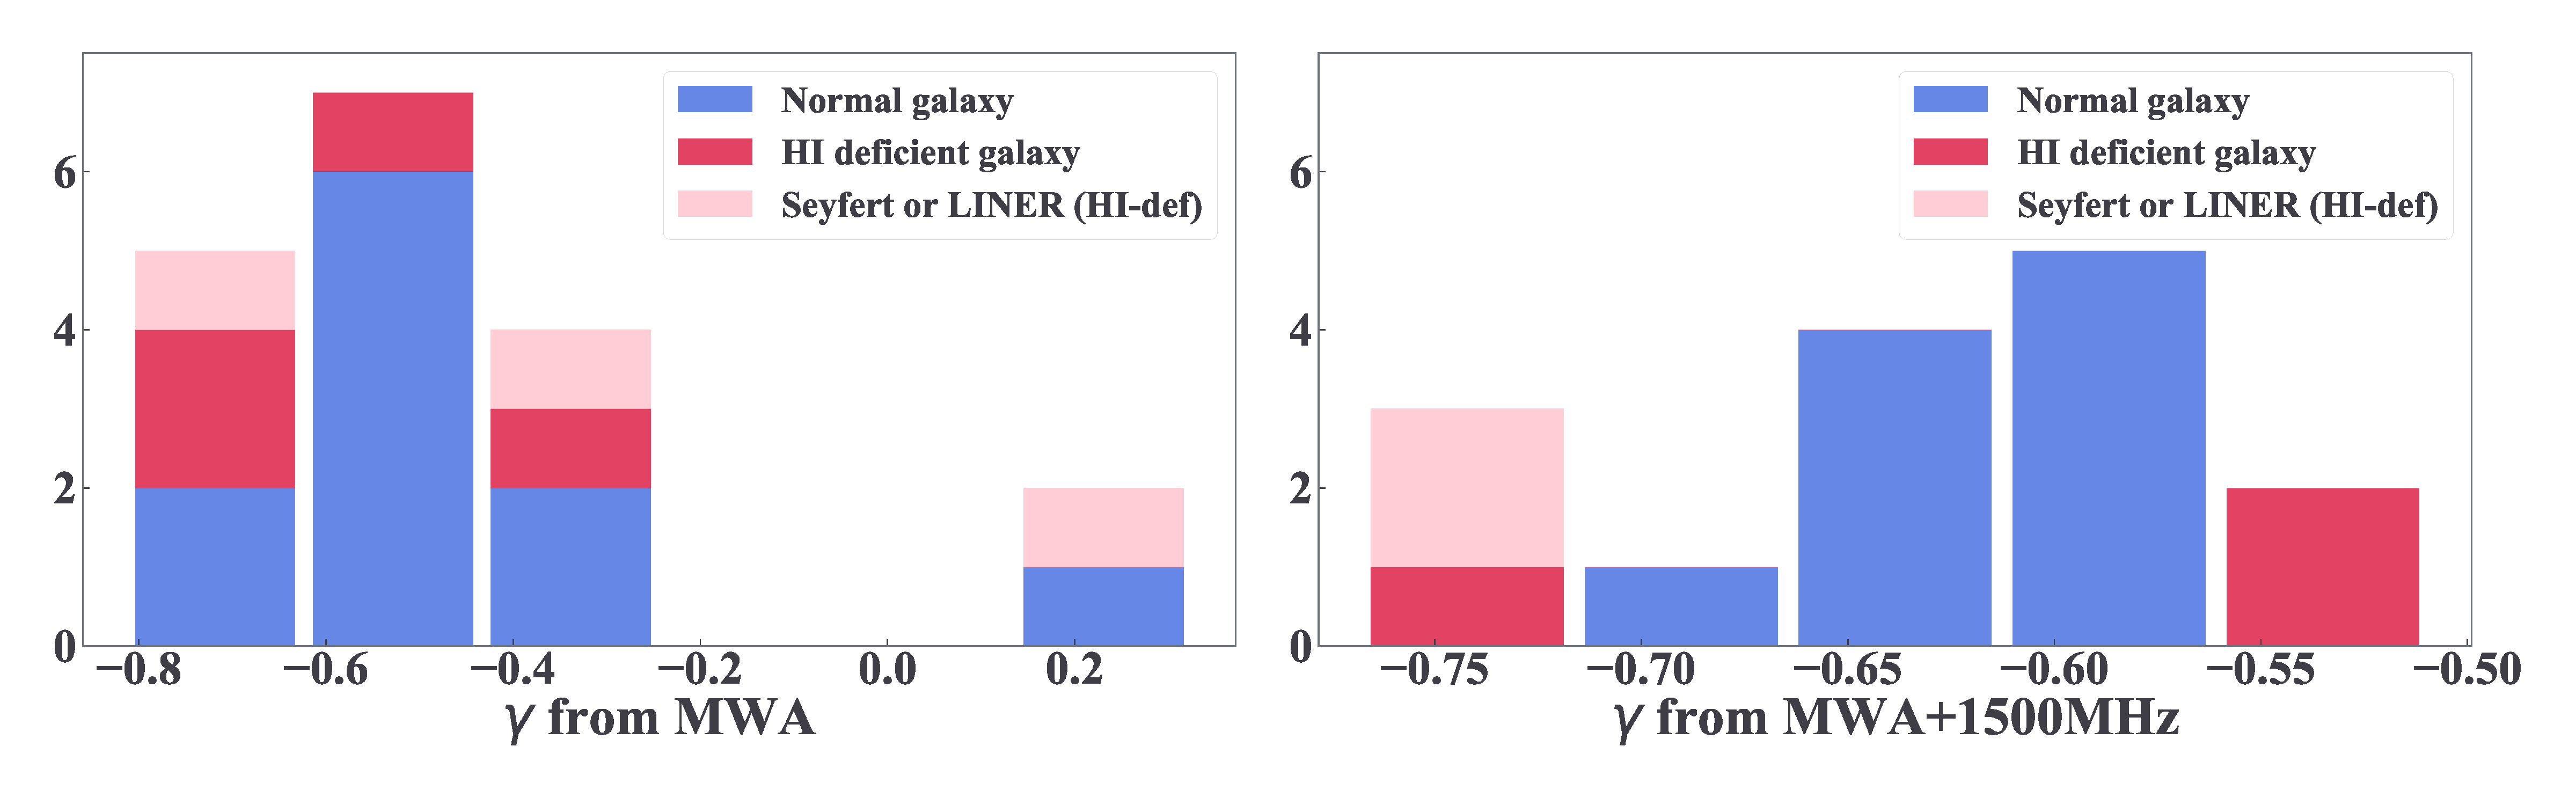
\includegraphics[width=\linewidth]{Chapter_6/Figures/Discuss_comparehist.pdf}
    \caption[Histograms of $\gamma$ from the fitting (labeled)]{\label{fig:comparehist_h1def}
        The spectral index distribution obtained from the two kinds of fitting as same as in Figure~\ref{fig:comparehist}.
        Here, we make a histogram with color labeling based on the galaxy properties mentioned in Section~\ref{sec:galaxypropertiesfortheradiosfr}.
        The blue histogram shows the normal galaxies; red one shows the HI deficient galaxies (\nh-def $> 0.4$), and the pink shows the Seyfert or LINER galaxies with \nh-deficient.
        Our sample does not have the galaxy, which is Seyfert or LINER without \nh-deficient.
        Although the left figure does not show the significant difference between normal galaxies and the others, the right figure shows the \nh~deficient galaxies tend to have a scatter spectral index compared to the normal galaxies.
    }
\end{figure}


Secondly, we show the $\qn$ value plots with the label of galaxy properties mentioned above.
This $\qn$ value plot helps us to understand how the galaxy property affects the SFR ratio in Figure~\ref{fig:sfrratio}.
As we have mentioned in Section~\ref{sec:sfrfromlowradio}, the $\qn$ value variation makes a larger scatter of SFR ratio when we estimate $\mr{SFR}_{\mr{Radio},\,\nu}$ with averaged parameters.

\begin{figure}[htbp]
	\centering
	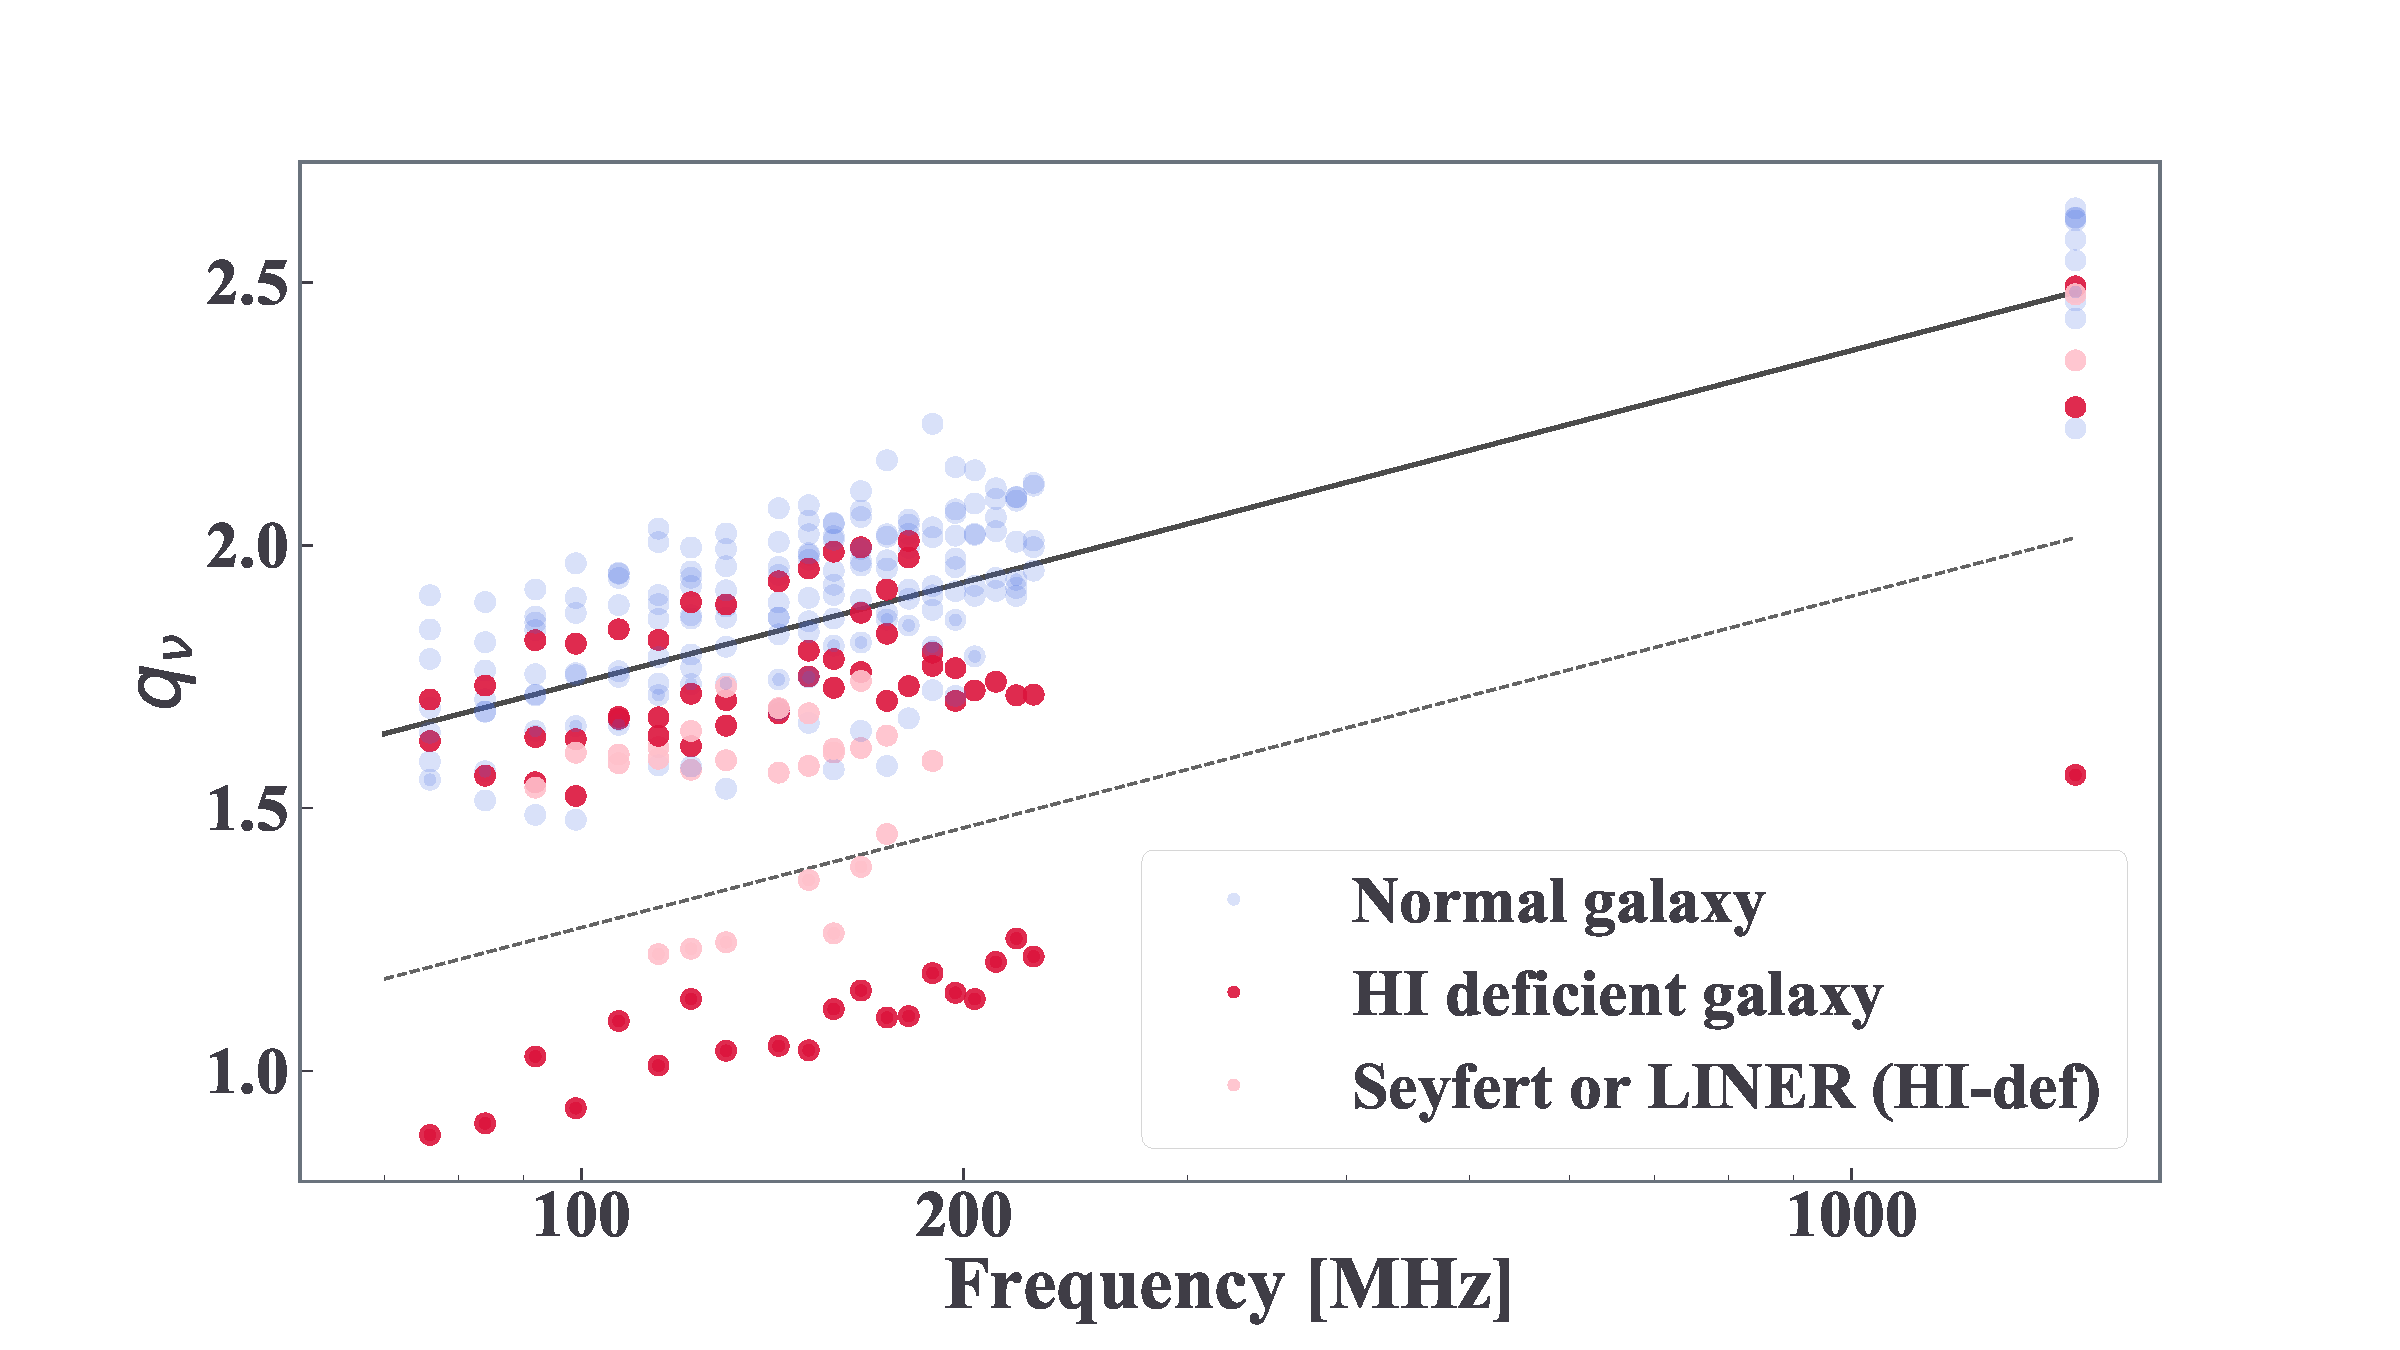
\includegraphics[width=\linewidth]{Chapter_6/Figures/Discuss_compareq.pdf}
    \caption[$\qn$ plots for each galaxy with labels]{\label{fig:comparehist_q}
        The $q_{\nu}$ value distribution at MWA frequencies and $1500\MHz$.
        The solid black line is the extrapolate line from the median value of $\q{1500\MHz}$ to the MWA frequencies with the median spectral index $\gamma$.
        For calculating $\mr{SFR}_{\mr{Radio},\,\nu}$, we have used this extrapolation. The dotted black line is the border for showing the outliers below this line.
        The plots below this line arise from only two galaxies, and we can say these are the outliers.
        In this figure, we can see the most plots distributing around the solid black line, which shows the extrapolated median value from $\q{1500\MHz}$.
        But we also find there are two galaxies (HRS 163 and 306) that have lower values in a whole frequency range.
    }
\end{figure}

In Figure~\ref{fig:comparehist_q}, we can see some \nh-deficient galaxies and Seyfert or LINER galaxies tend to have smaller $\qn$ values, which means they have stronger radio emissions.
As I have already mentioned, \nh-deficient galaxies would have amplified synchrotron radiation caused by the distortion of their magnetic field.
Figure~\ref{fig:comparehist_q} shows that \nh-deficient galaxies including AGNs have relatively smaller $\qn$ (stronger radio emission), and this result might support the scenario.
We also find that there are two galaxies (HRS 163 and 306), which have significantly lower $\qn$ values.
Since galaxies which have stronger radio emissions might possess the other radio source rather than the star formation activity in addition to the effect of the magnetic distortion, we should not estimate SFR from radio emissions for these galaxies.
Indeed, these two galaxies are outliers on the right plot in Figure~\ref{fig:sfrratios} and apparently these make non-negligible uncertainty.

For the reliable SFR estimation with the low-frequency emission, we definitely need to classify which galaxies are appropriate for calculating their SFR from radio emissions.
However, due to our sample size, we cannot conclude how much $\qn$ value is safe for executing the SFR estimation from the low-frequency emission.
In future studies, we should clarify the distribution of this plot and find borders of $\qn$ for reliable SFR estimation.


\section{Non-detected Galaxies by the GLEAM Survey}\label{sec:nondetectedgalaxiesbythegleamsurvey}

Here, we mention galaxies that have not been observed by the GLEAM survey.
In this study, we have found 39 HRS galaxies have a potential radio counterpart in the GLEAM survey in Section~\ref{sec:crossmatching}.
So in this Section, we focus on other 283 HRS galaxies.

Firstly, we check the coordinate of these galaxies, and peeled sources which was removed during the data reduction for compiling the GLEAM catalog.
Out of 283 galaxies, we confirm 44 galaxies are out of the observational region by the GLEAM survey, and HRS 183 (M87, Virgo A) is peeled because of its too strong radio emission.
\citet{Hurley-Walker2017a} peeled radio sources expected to be more than $50\,\mr{Jy}$ in apparent flux density from the visibilities for reducing the grating sidelobes.
So we confirm these 45 galaxies have reasonable reasons why their radio sources are not on the GLEAM catalog.
However, the other 238 out of 283 galaxies do not have understandable reasons.

Secondly, we examine the flux values at $200\MHz$ because their non-detection is reasonable if the expected flux value is lower than the detection limit.
In this analysis, we extrapolate the flux at $200\MHz$ from $1500\MHz$ \citep{Boselli2015} with $S \propto \nu^{\gamma}$ $\brp{\gamma = -0.63\ \text{obtained in this study}}$ and compare it with the rms noise described in \citet{Hurley-Walker2017a}.
Note that the rms noise is different depends on the declination, so we apply $\sigma\msb{rms} = 10$ for galaxies at $-72^{\circ} \leq \mr{Dec} \leq 18^{\circ}.5$ and $\sigma\msb{rms} = 28$ for galaxies at $18^{\circ}.5 \leq \mr{Dec}$.
Also, we should mention that we can analyze only 107 galaxies because other the 131 galaxies do not have a high-quality flux data at $1500\MHz$ \citep{Boselli2015}.
After all, we find 34 galaxies have extrapolated flux at $200\MHz$ higher than $5\sigma\msb{rms}$.
This result means that these 34 galaxies should have been observed by the GLEAM survey, but they were not.
One possible reason for the non-detection of these galaxies is a flatter radio spectral.
Here, we assume $\gamma = -0.63$ for the extrapolation.
However, if these galaxies have a flatter spectral, the flux of these galaxies at $200\MHz$ is smaller than the expected value and they are not detected.

In the GLEAM-X survey, which is the follow-up observation of the GLEAM survey, more than 50 HRS galaxies will be detected even their spectral index is $\gamma = \pm 0$ because of the roughly ten times higher sensitivity of the coming up survey.
This survey also has $\sim 10$ times higher angular resolution, so that we will be able to improve our study, especially to investigate the effect of compact regions in star-forming galaxies.



%\bibliographystyle{mnras}
%%\bibliography{example} % if your bibtex file is called example.bib
%\bibliography{masterthesis}

    \chapter{Summary and Future prospects}\label{chap:summary}
%\begin{chapabstract}
%
%Intro intro intro intro.
%
%\end{chapabstract}

In this study, we investigate 18 star-forming galaxies in the HRS catalog for their global relation of the low-frequency radio with IR luminosities.
We find a single power-law assumption for the frequency dependence of $\qn$ is valid across MWA frequencies and $1.5\GHz$, and their slope $\gamma$ is consistent with previous studies.
We also investigate the consistency of the radio SFR expected to be an extinction-free indicator with SFR calculated from other indicators.
In this study, we calculated the radio SFR in two ways.
The first one is to use individual $\q{1500\MHz}$ and $\gamma$ for calculating SFR.
In this case, the radio SFR is consistent with $\mr{SFR}\msb{IR}$ within $20\%$ error.
Another one is to use the averaged $\q{1500\MHz}$ and $\gamma$ and derive the calibration applied for all galaxies.
This calibration gives us one calibration equation and we can calculate SFR even we have only a single band luminosity.
However, this calibration has a two times more significant error than the former one although it is consistent with $\mr{SFR}\msb{IR}$.

These results suggest that the spectral information for each galaxy is needed to estimate its SFR accurately because of a wide variety of $\qn$.
After all, we propose that future observation with several radio bands is required at low frequencies for measuring accurate SFRs.

For further understanding of the low-frequency properties in star-forming galaxies, we need more samples from multi-band observation.
The updated GLEAM survey will reveal physical details with an order of magnitude better angular-resolution and sensitivity than the latest survey.


%%%%%%%%%%%%%%%%%%%% REFERENCES %%%%%%%%%%%%%%%%%%

% The best way to enter references is to use BibTeX:

\bibliographystyle{mnras}
%\bibliography{example} % if your bibtex file is called example.bib
\bibliography{masterthesis}

%%%%%%%%%%%%%%%%%%%%%%%%%%%%%%%%%%%%%%%%%%%%%%%%%%

\appendix

\chapter{Galaxy images}\label{chap:galaxyimages}

\section{Matched samples (18 samples used for the analysis)}
\begin{figure}[htbp]
	\centering
	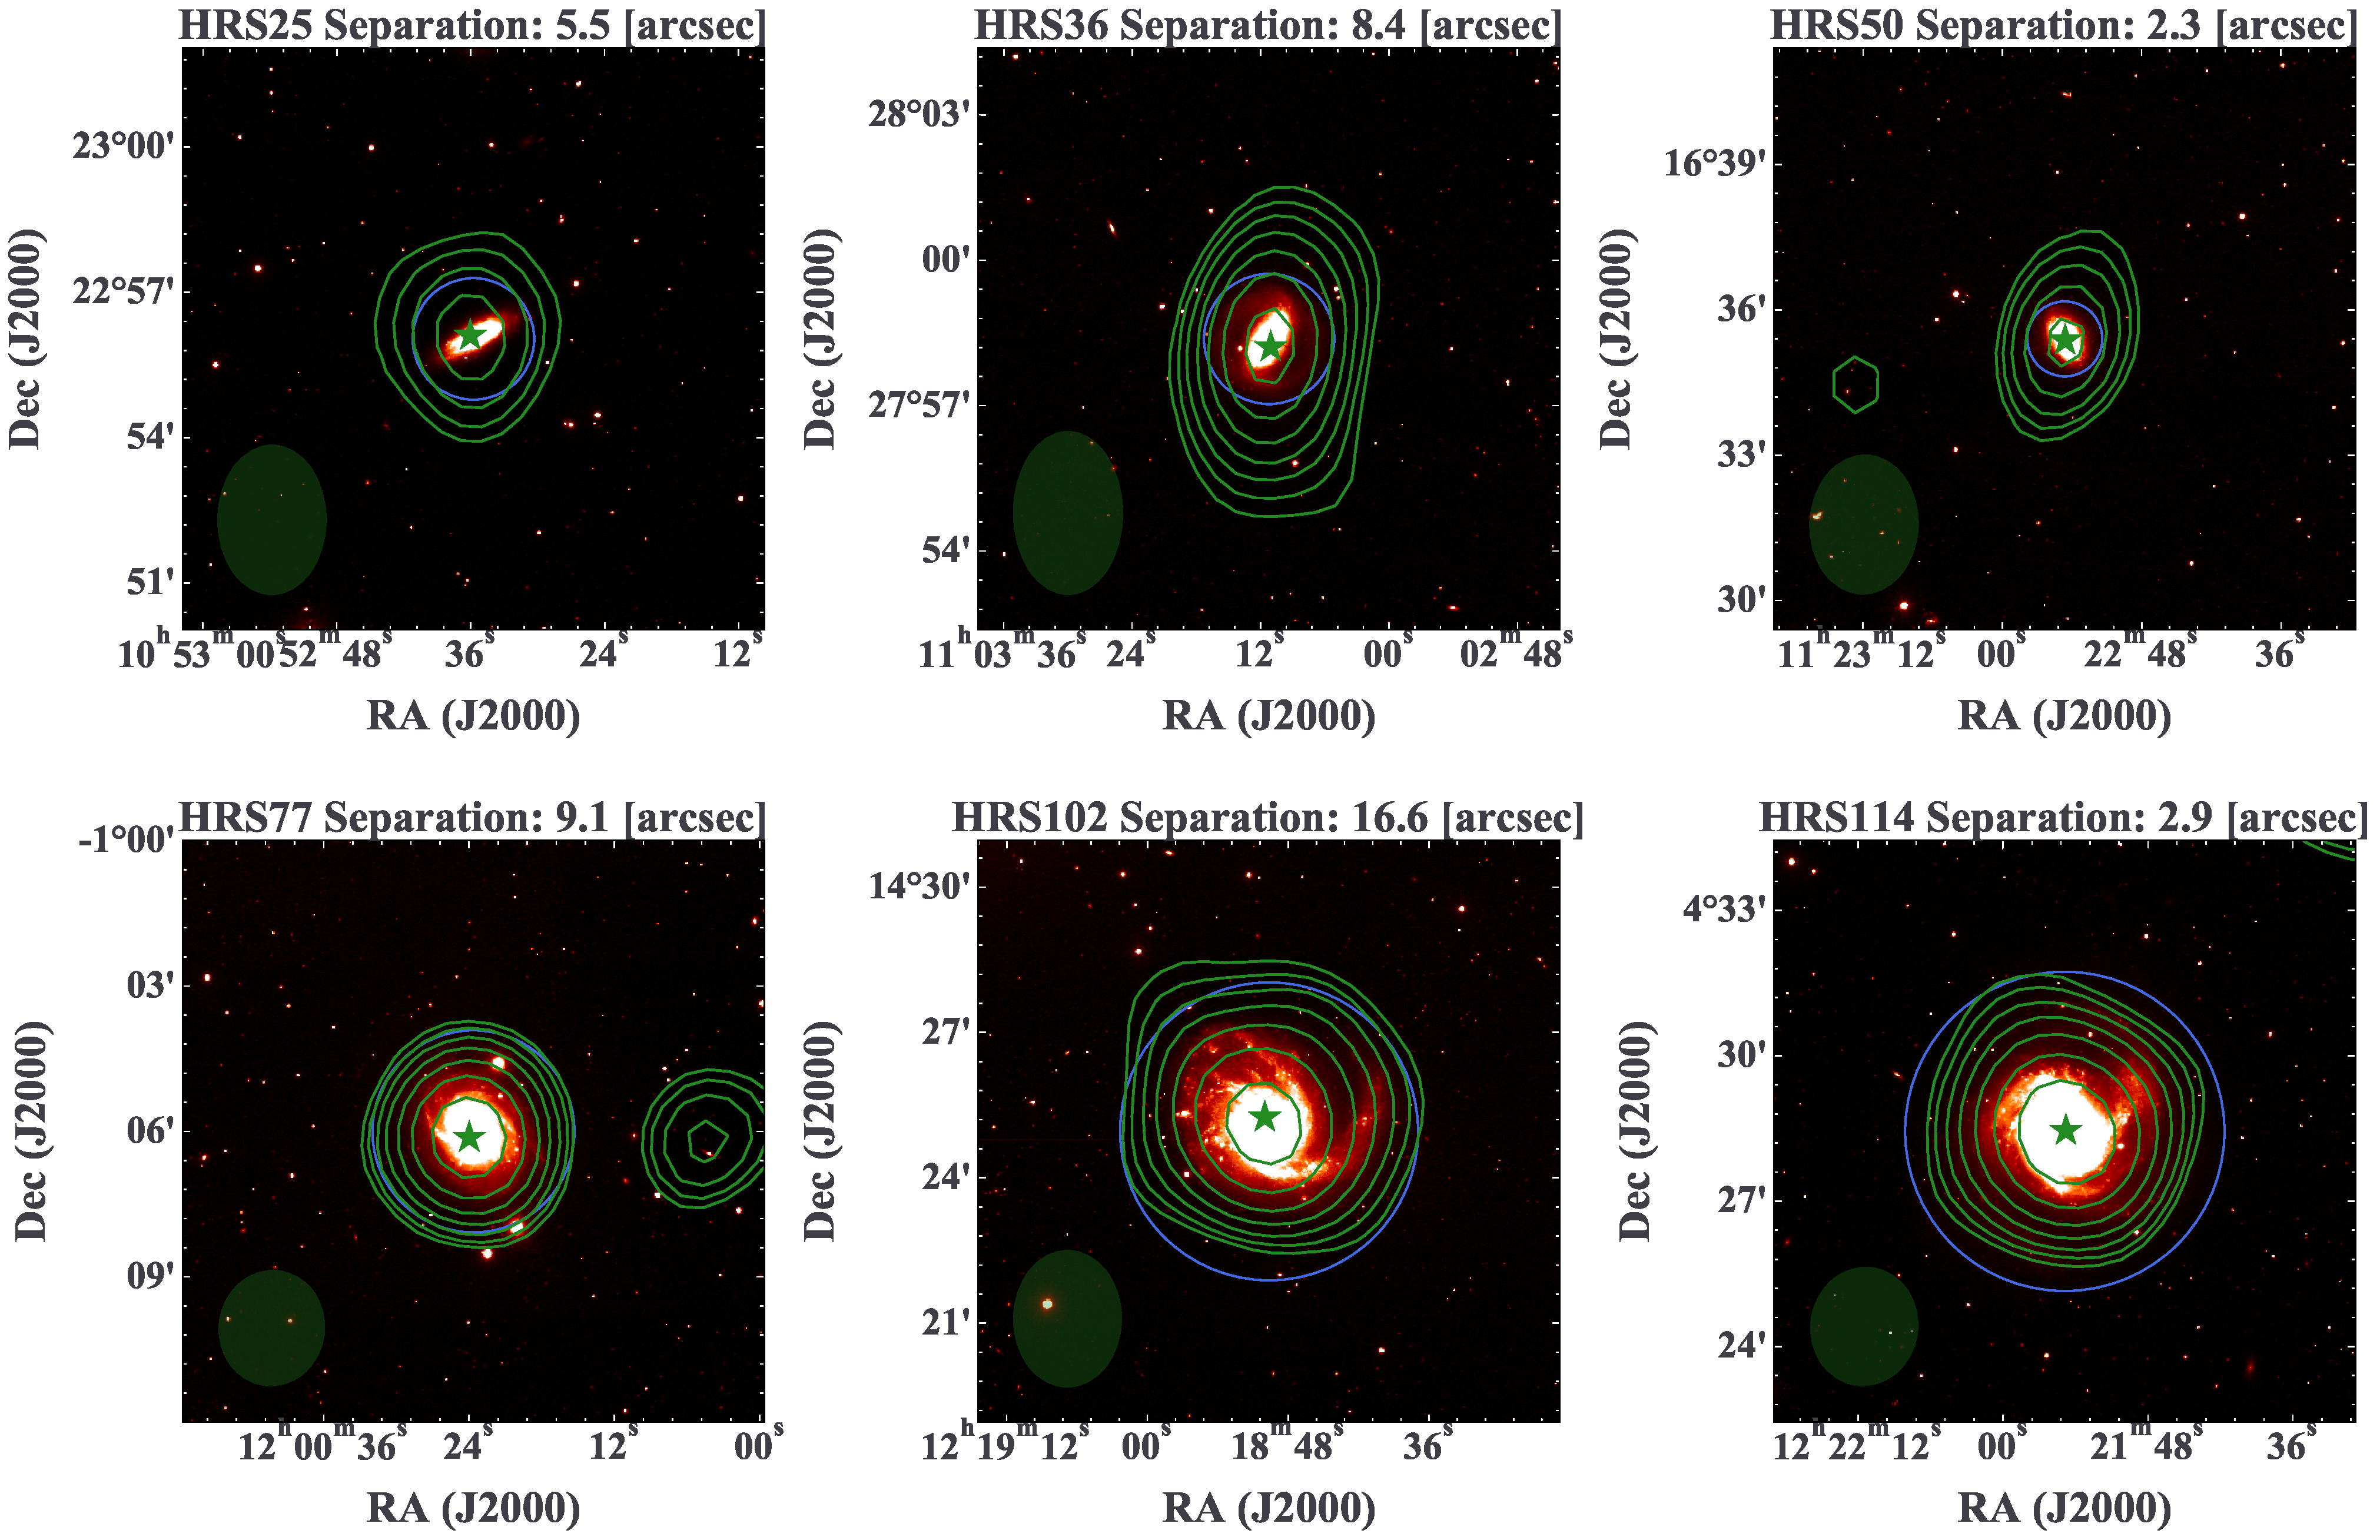
\includegraphics[width=\linewidth]{Figures/AppendixB_galaxyimages.pdf}
    \caption[Galaxy images (6/18 used for the analysis)]{\label{fig:galaxyimages}
        These are the SDSS \citep{Abolfathi2018} i-band images with radio contours from the GLEAM survey at $170-231\MHz$ (solid green lines).
        These galaxies are selected in Section~\ref{sec:crossmatching} and~\ref{sec:reducegalaxysamples}.
        I draw the green contours started from the 3$\sigma$ local noise and increase by a factor of the square root of $2^n$ (``n'' is an integer).
        The green star marker shows the location of a radio source referred to as the GLEAM catalog.
        The size of this marker does not mean any feature of observations.
        The blue circle shows the isophotal optical size at $25\,\mr{mag}\arcs^{-2}$ from \citet{Boselli2010}.
        On the bottom left in each plot, we show the beam size of the GLEAM survey.
    }
\end{figure}

\begin{figure}[htbp]
    \centering
    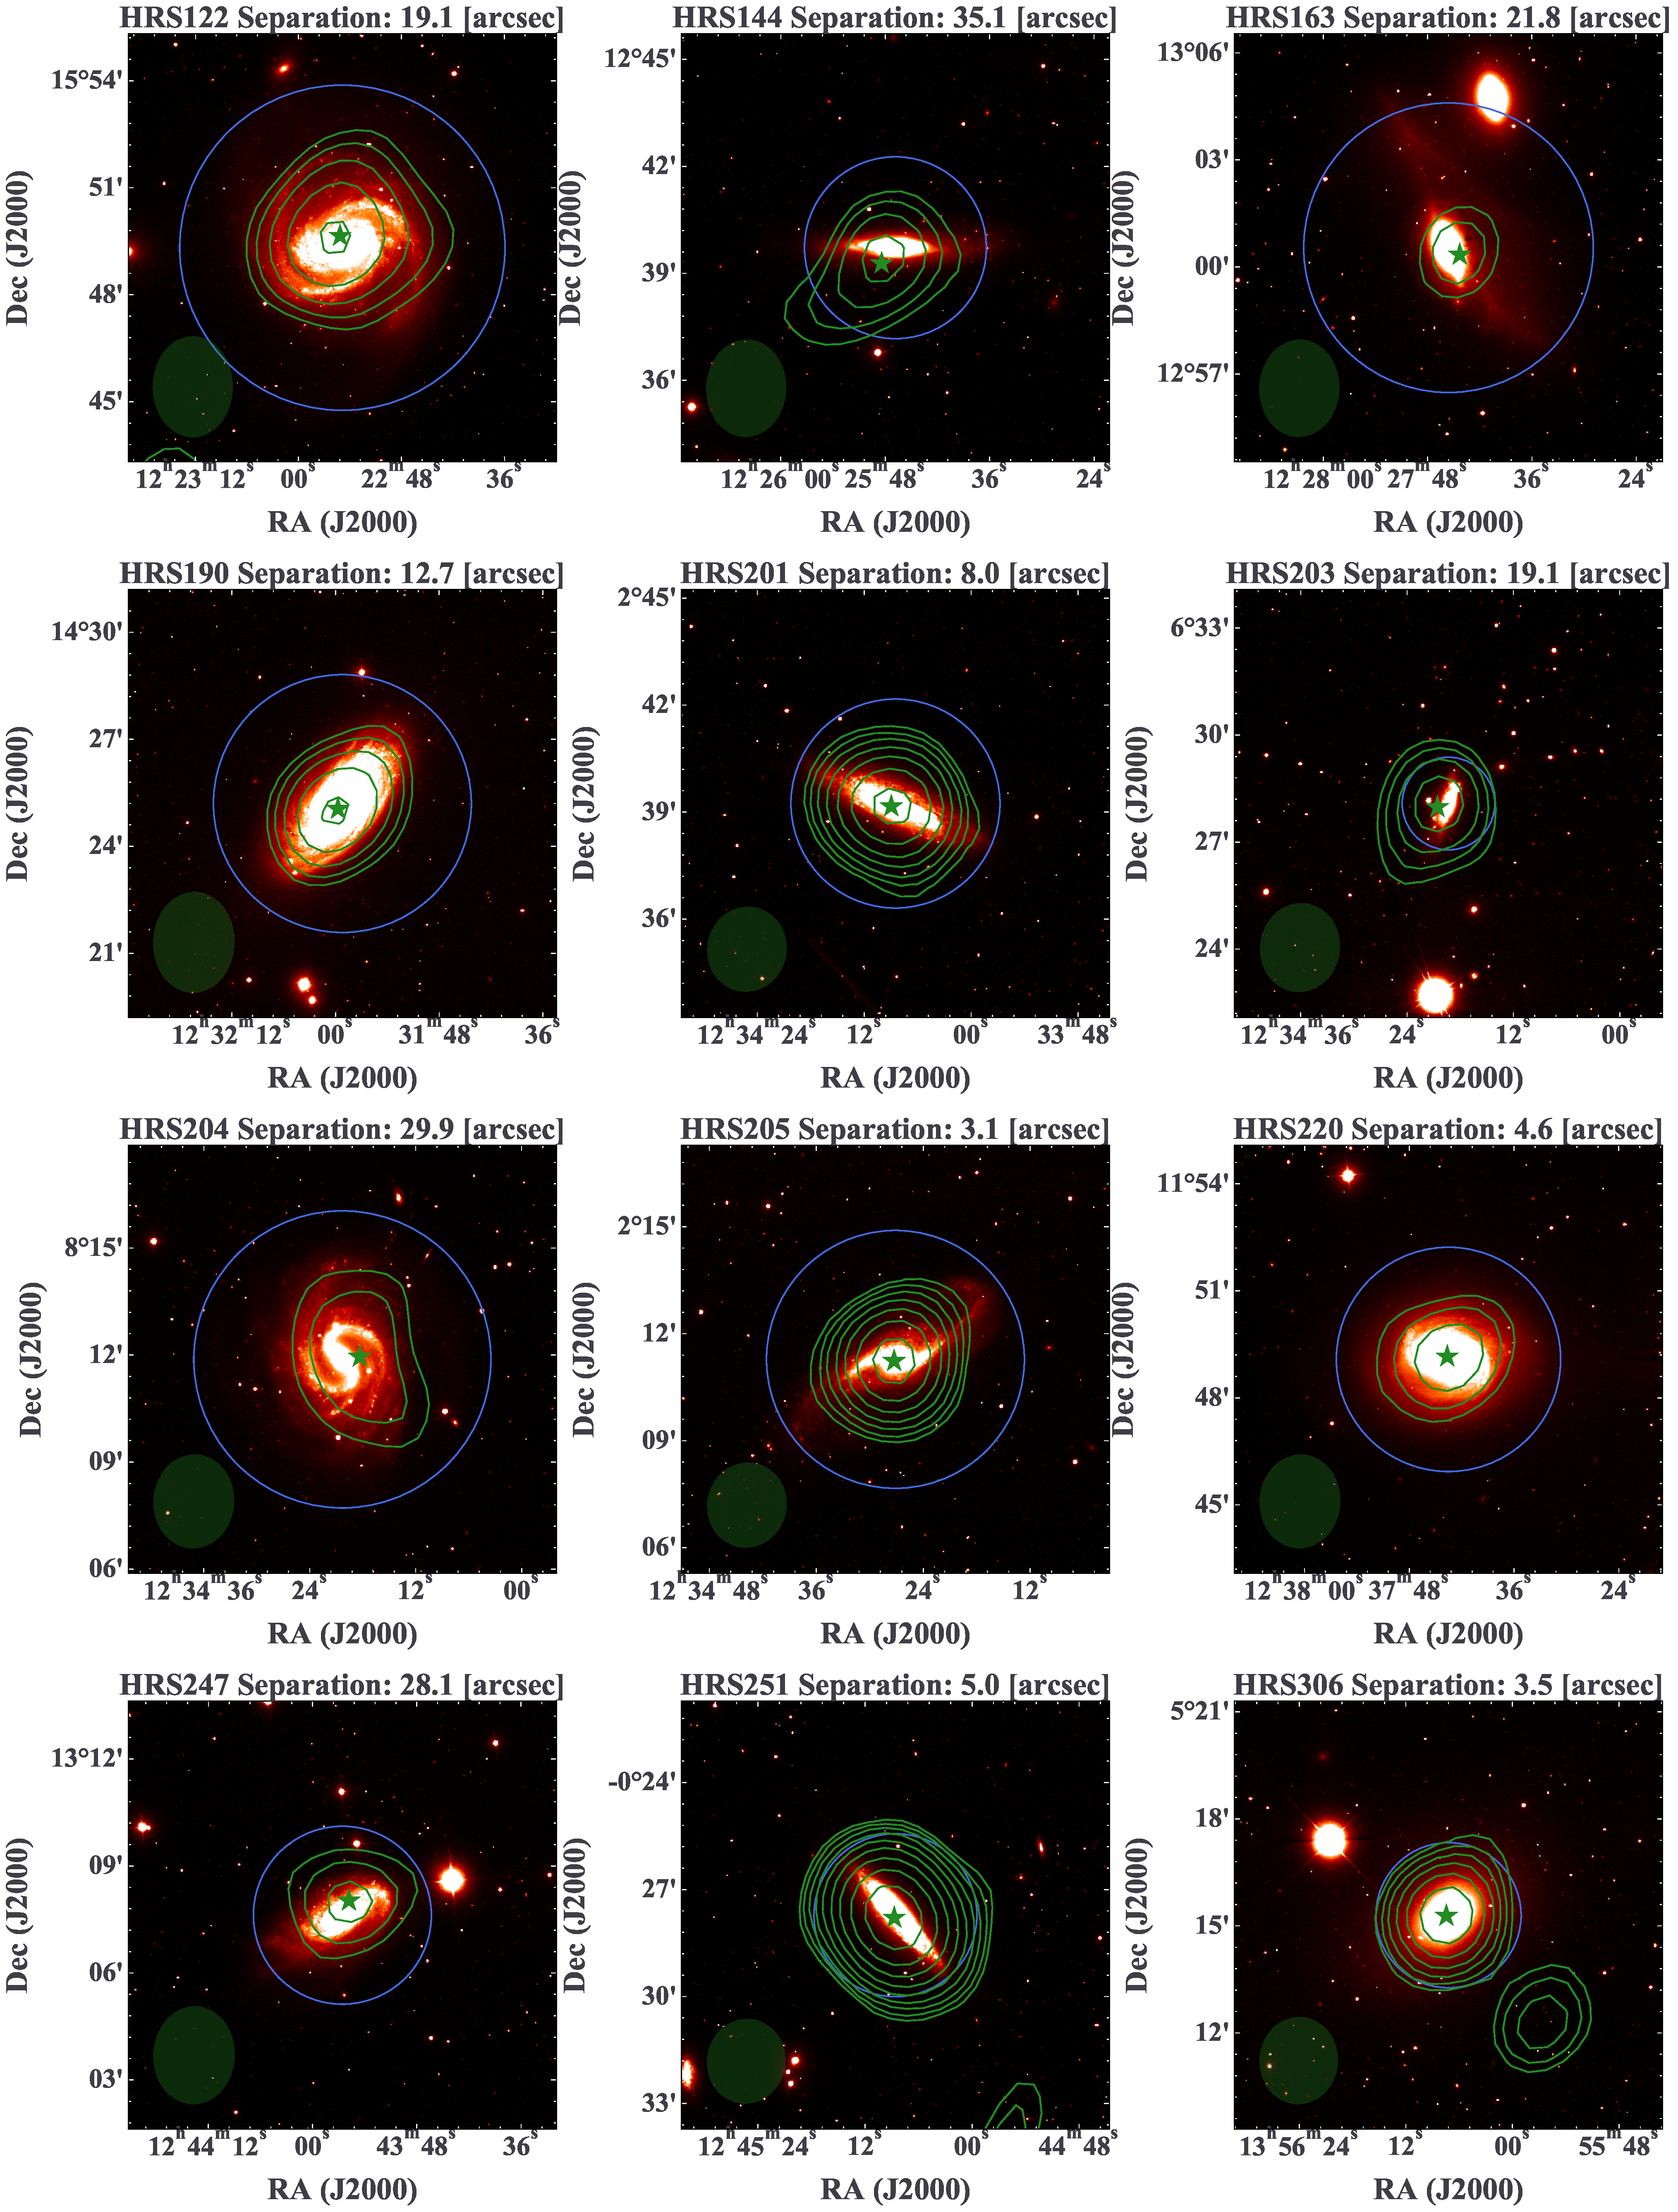
\includegraphics[width=\linewidth]{Figures/AppendixB_galaxyimages2.pdf}
    \caption[Galaxy images (12/18 used for the analysis)]{\label{fig:galaxyimages2}
        Continuous.
    }
\end{figure}



\section{Matched samples (not used for the analysis)}
\begin{figure}[htbp]
    \centering
    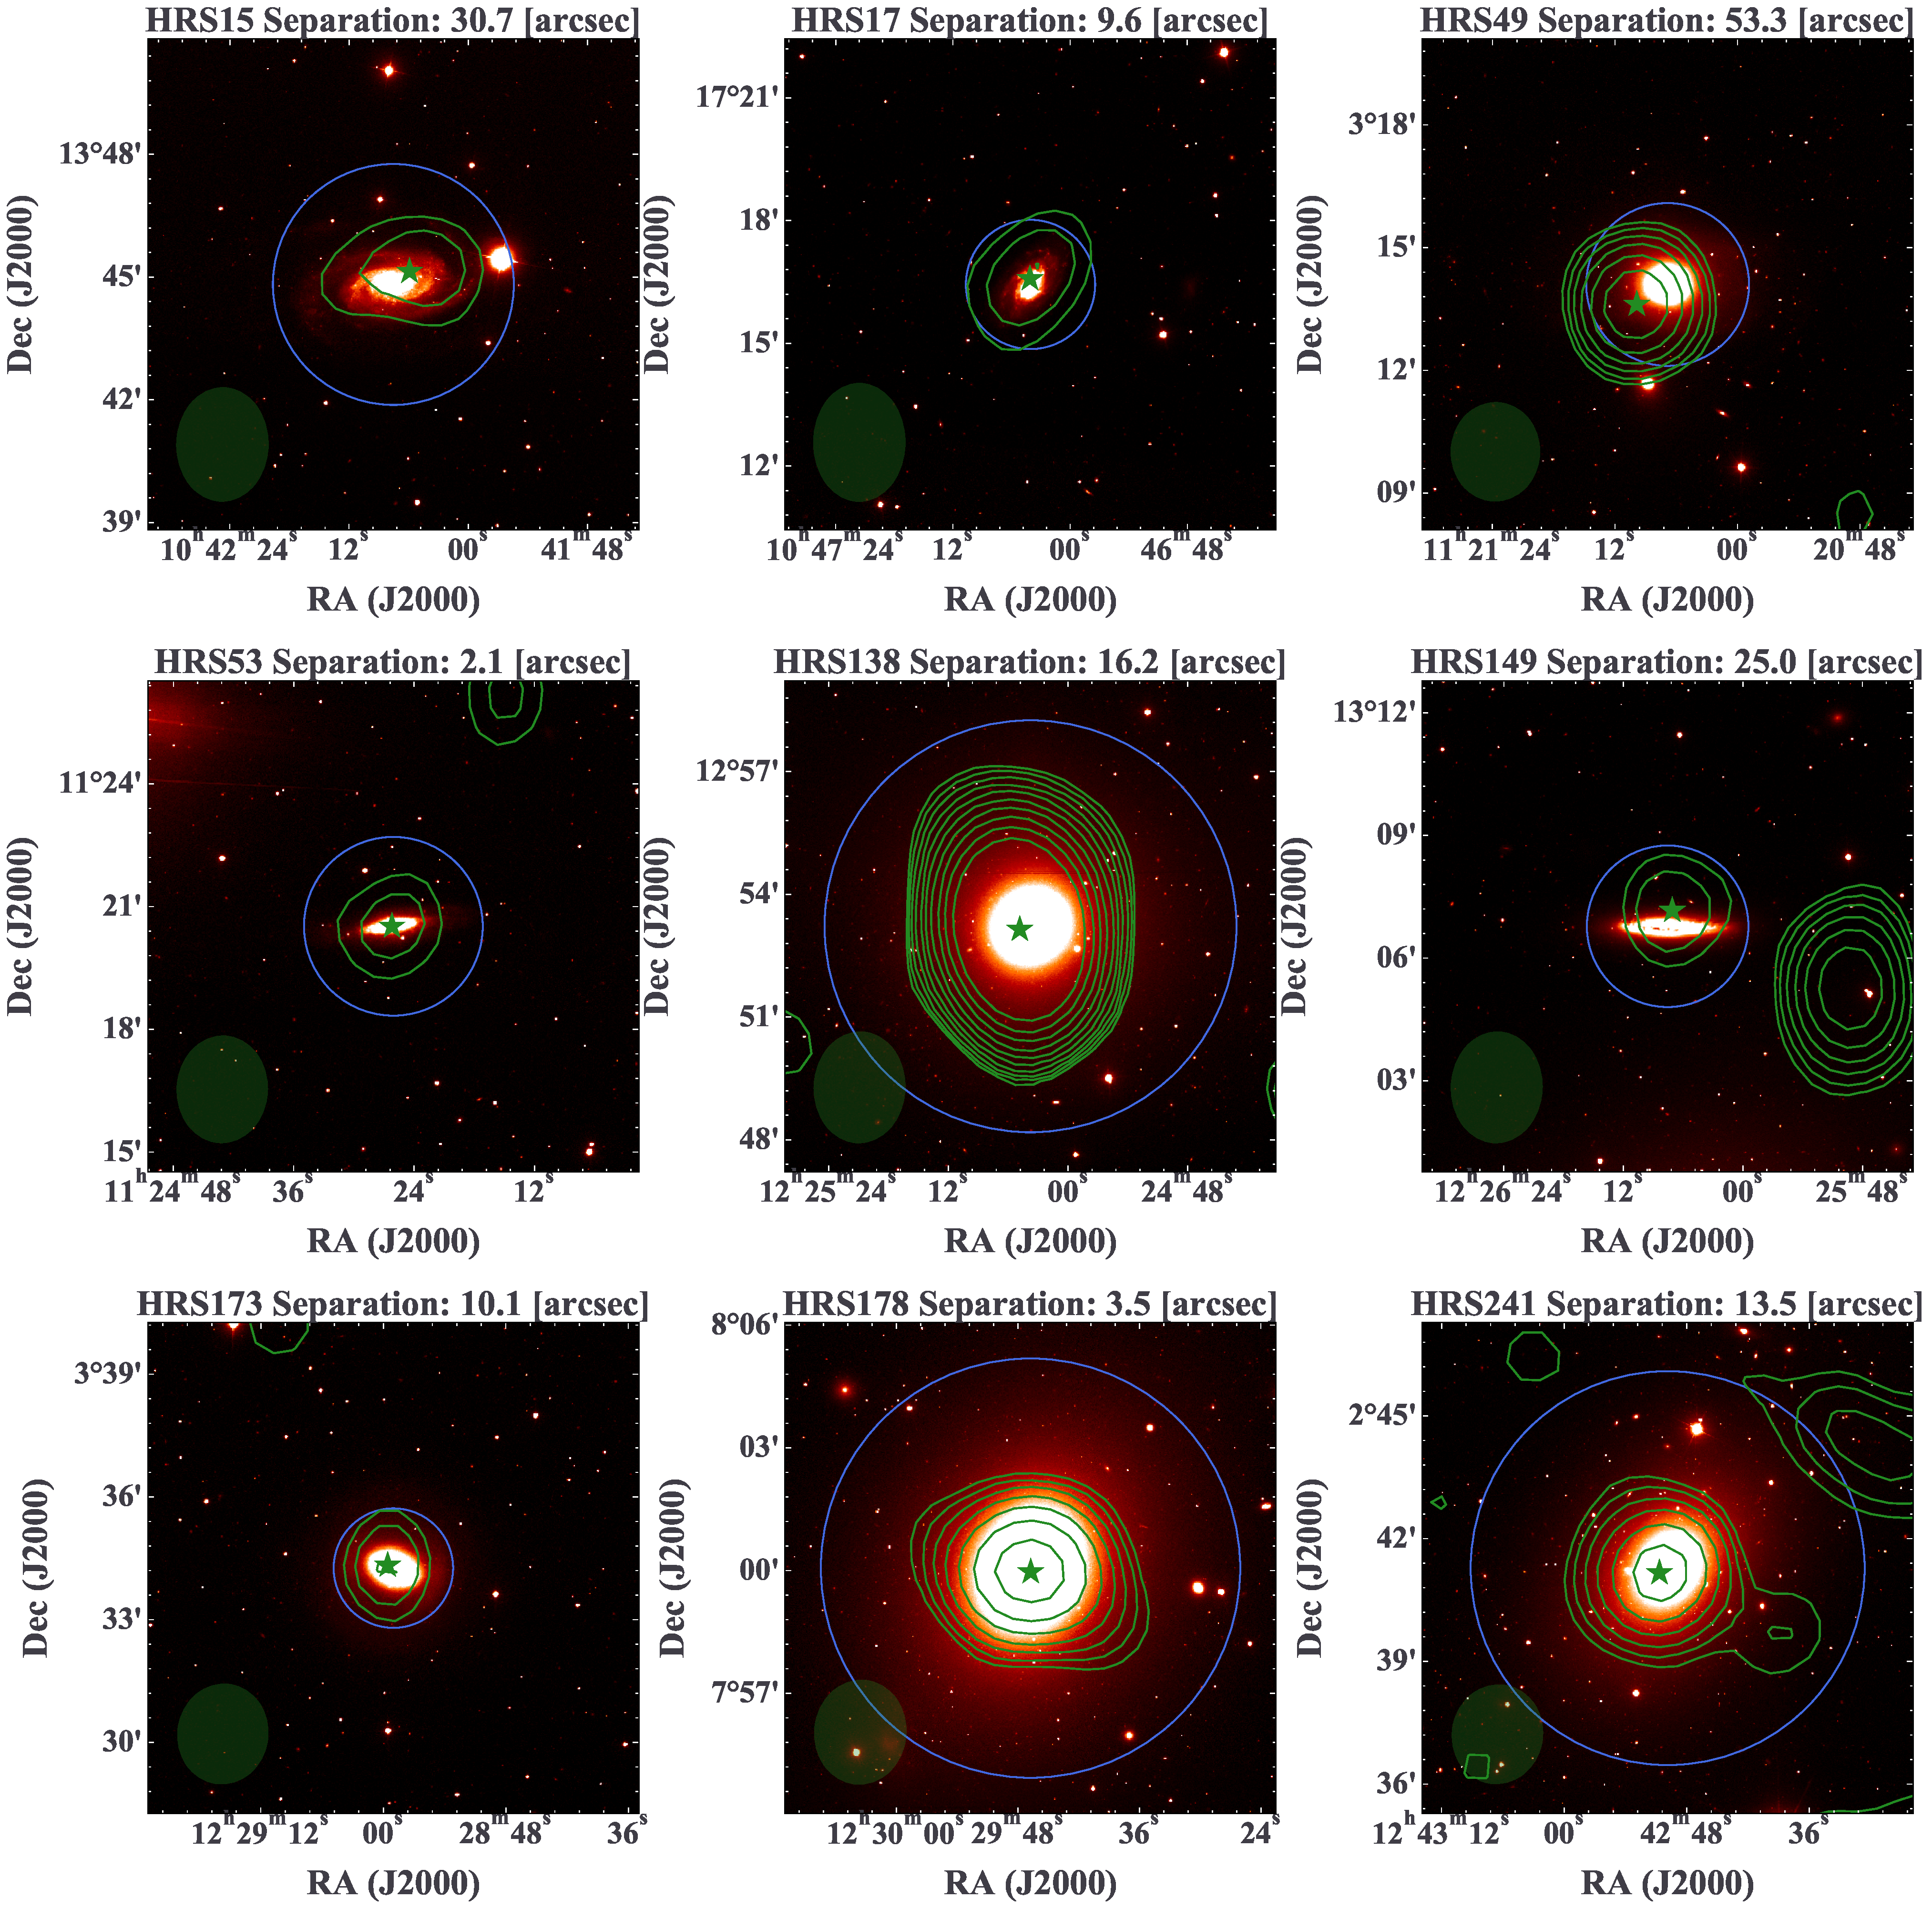
\includegraphics[width=\linewidth]{Figures/AppendixB_galaxyimages_notselected.pdf}
    \caption[Galaxy images (9/15 not used for the analysis)]{\label{fig:galaxyimages_notselected}
        These galaxies are not used for the analysis labeled in Section~\ref{sec:reducegalaxysamples} although they have a radio counterpart in the GLEAM catalog by the cross-matching.
    }
\end{figure}

\begin{figure}[htbp]
    \centering
    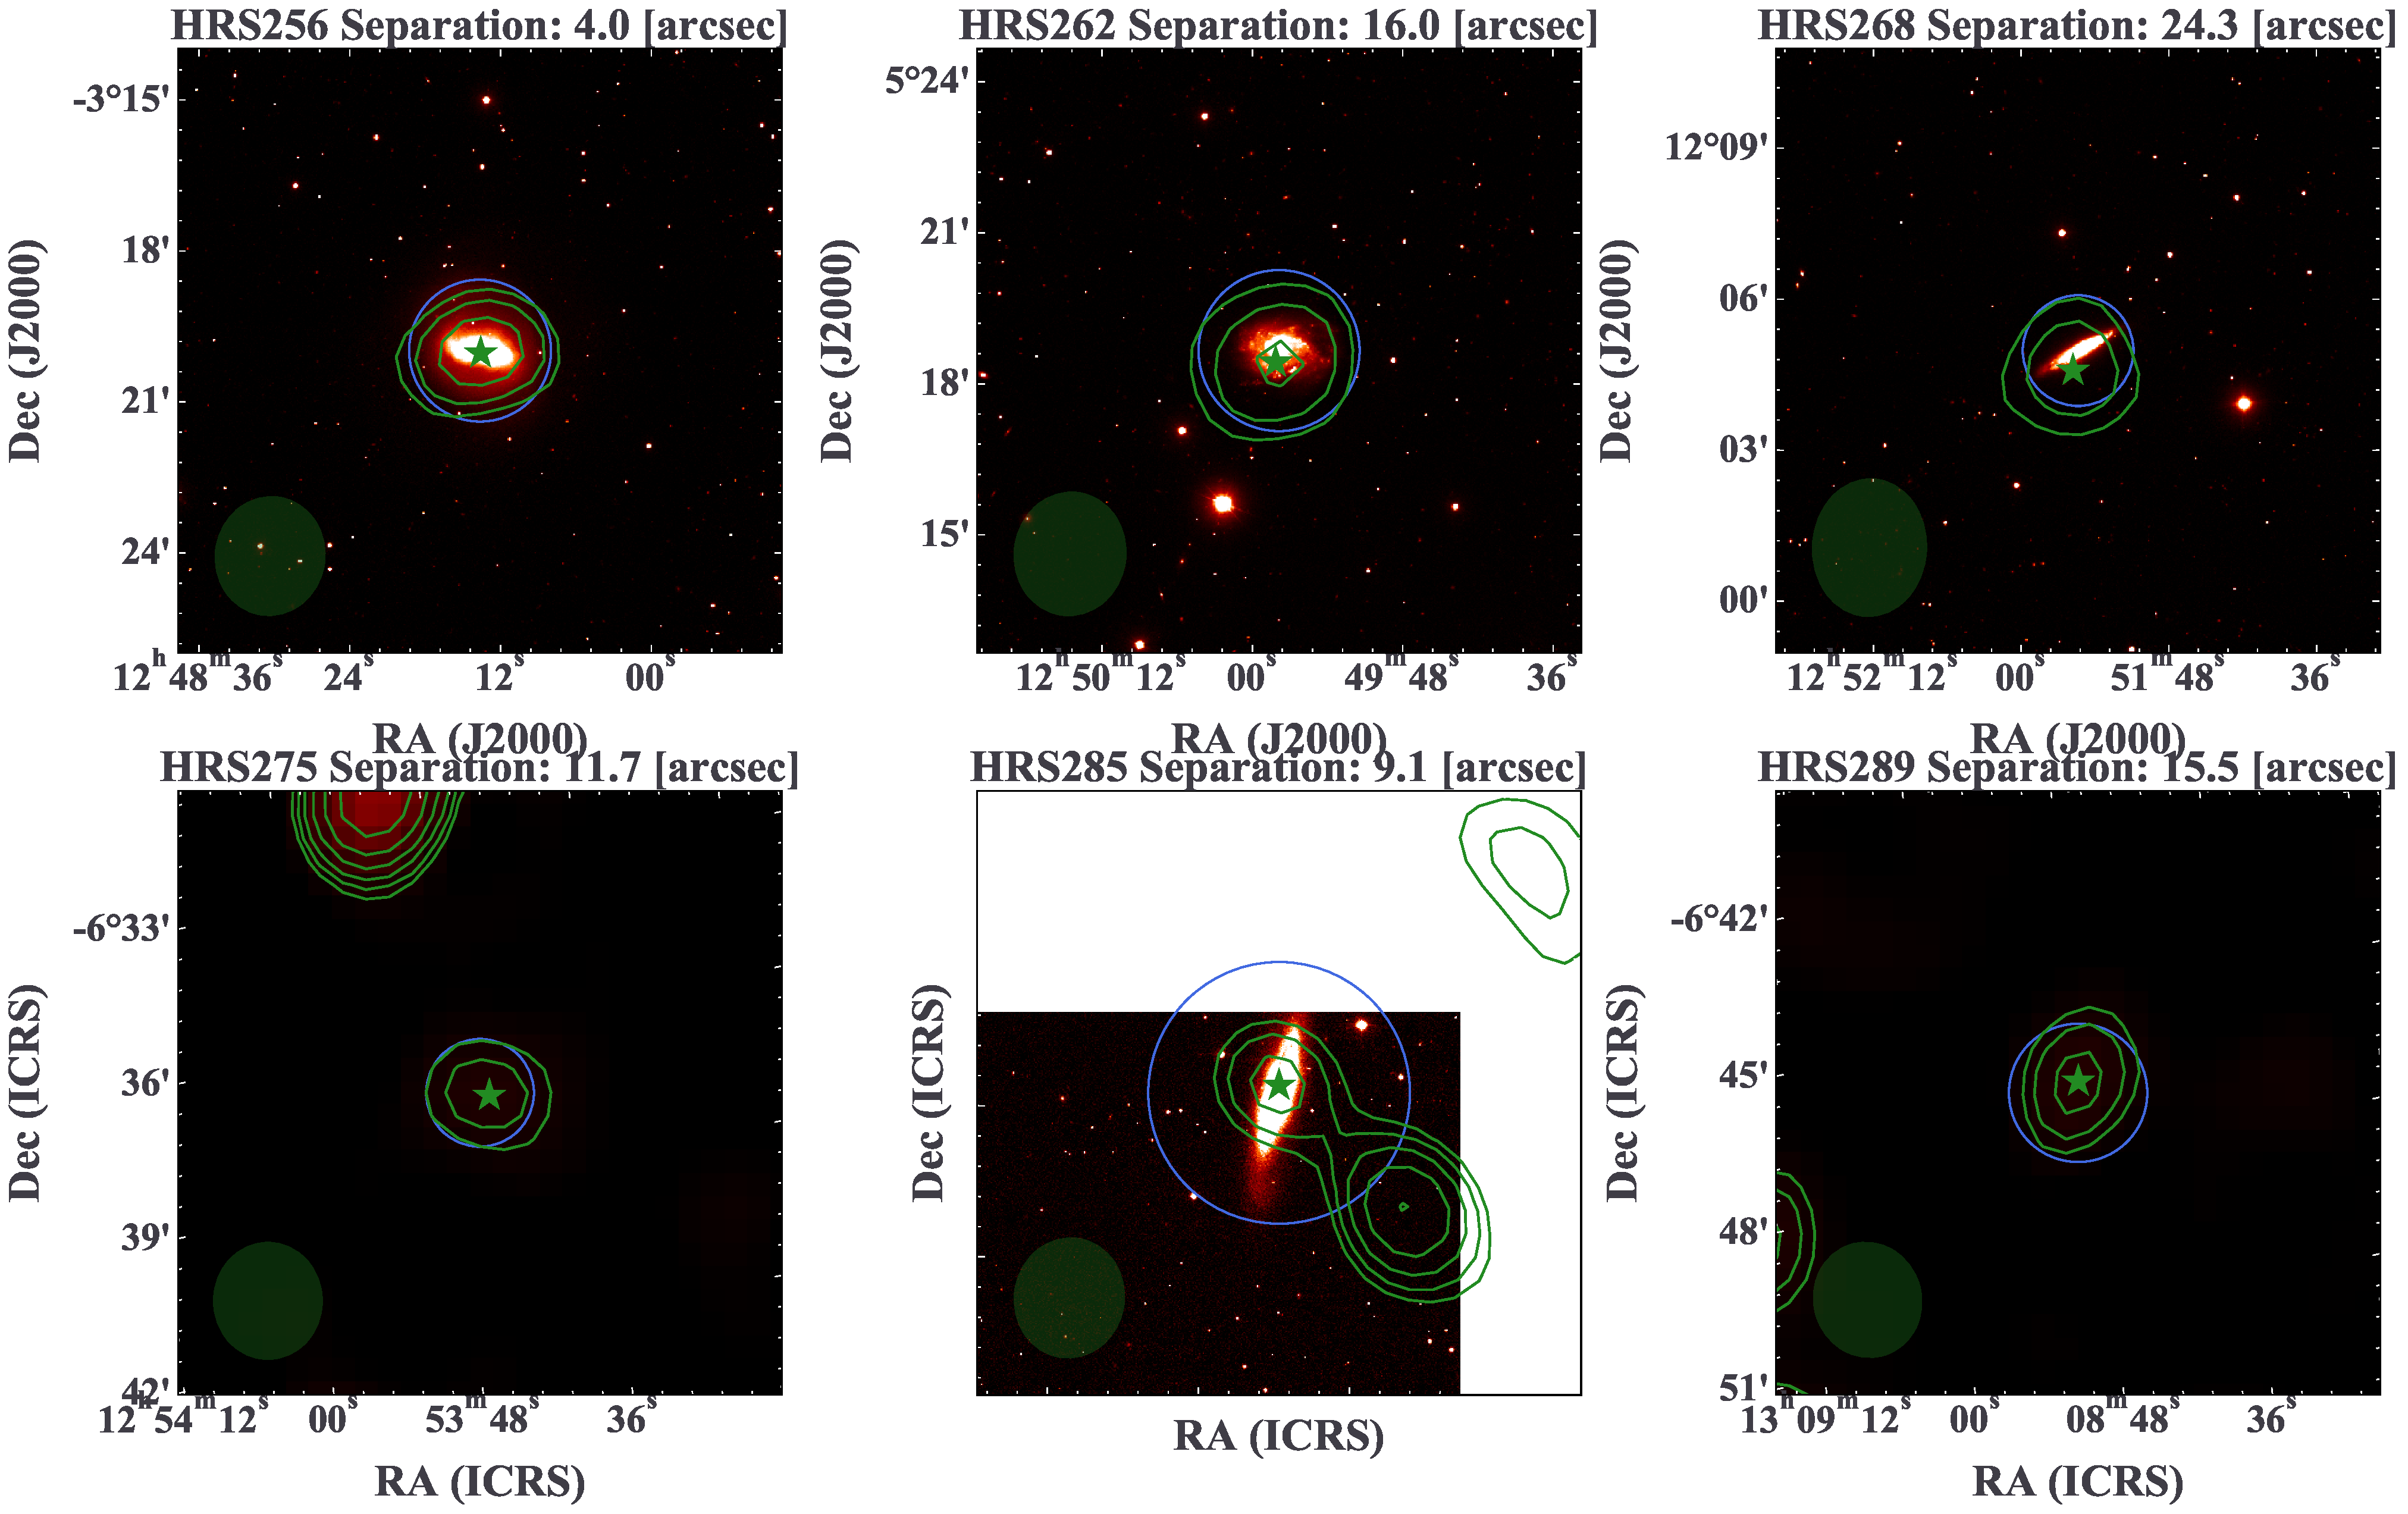
\includegraphics[width=\linewidth]{Figures/AppendixB_galaxyimages_notselected2.pdf}
    \caption[Galaxy images (6/15 not used for the analysis)]{\label{fig:galaxyimages_notselected}
        Continuous.
    }
\end{figure}



\section{Suspicious matching samples}
\begin{figure}[htbp]
    \centering
    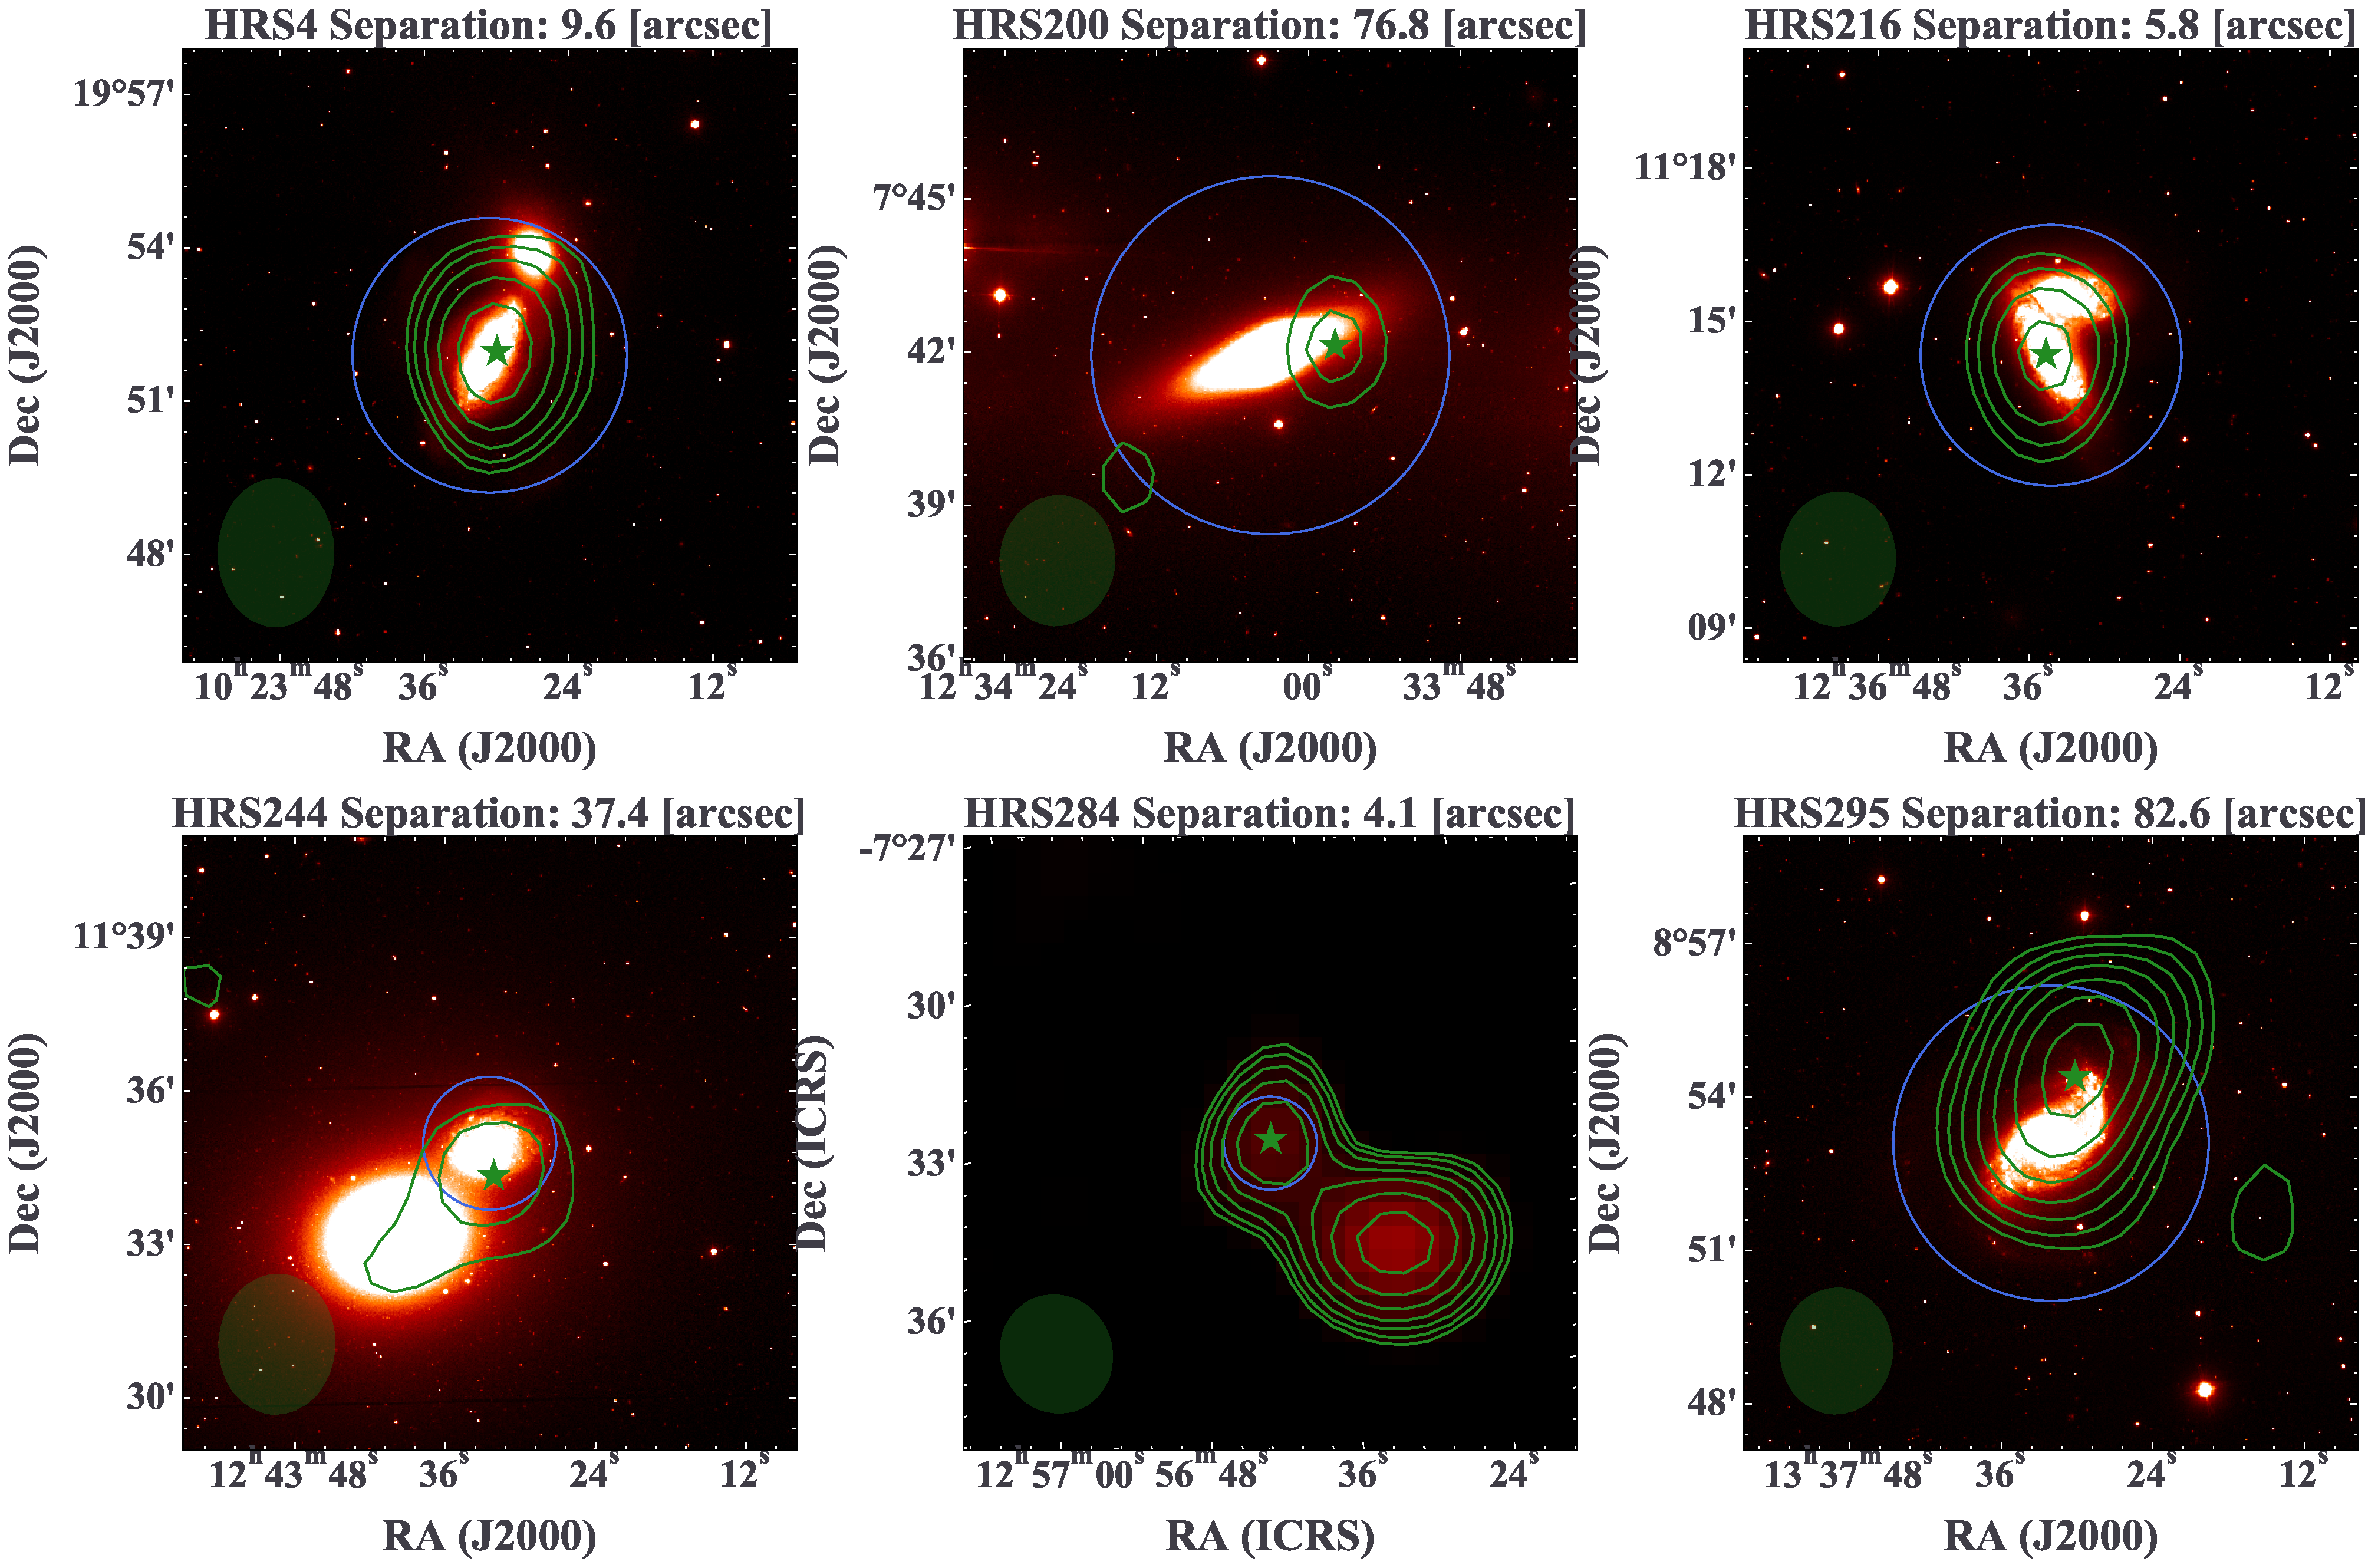
\includegraphics[width=\linewidth]{Figures/AppendixB_galaxyimages_suspicious.pdf}
    \caption[Galaxy images (suspicious matching)]{\label{fig:galaxyimages_suspicious}
        These galaxies are flagged as a suspicious matching in Section~\ref{sec:crossmatching}
    }
\end{figure}



\section{Not matching samples}
\begin{figure}[htbp]
    \centering
    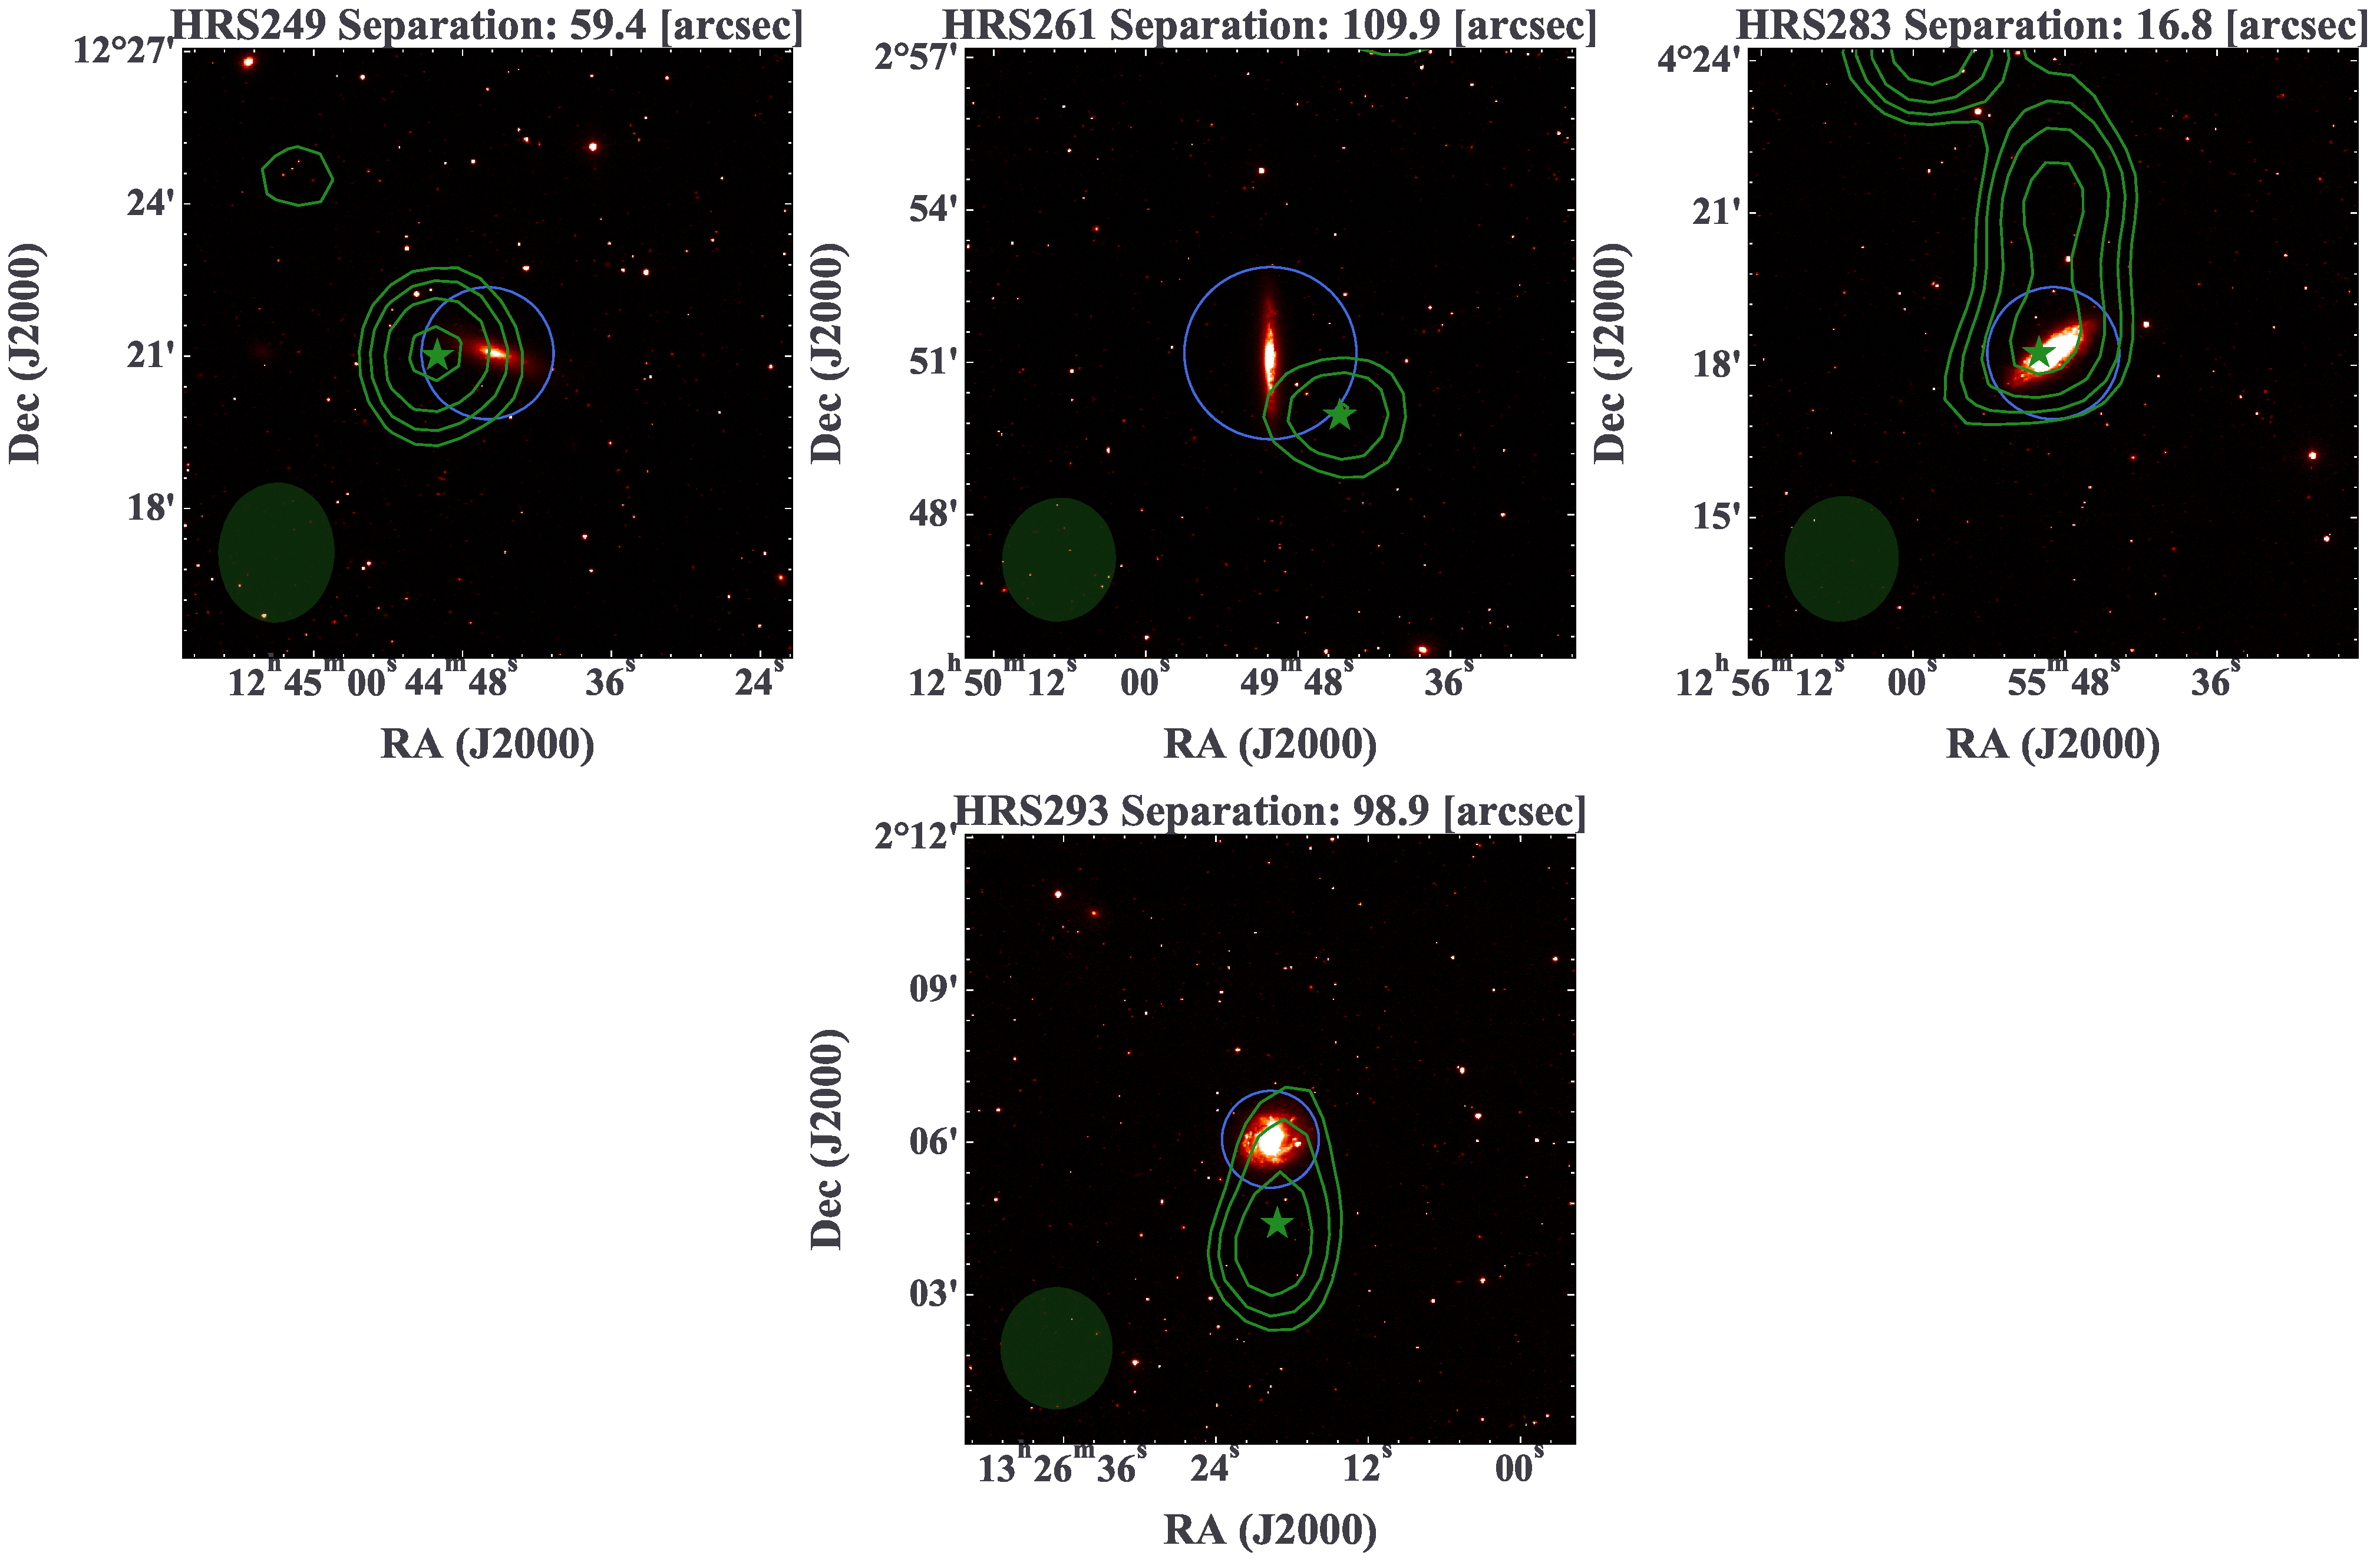
\includegraphics[width=\linewidth]{Figures/AppendixB_galaxyImages_noMatch.pdf}
    \caption[Galaxy images (no matching)]{\label{fig:galaxyimages_nomatch}
        These galaxies do not have a radio counterpart from the GLEAM catalog in Section~\ref{sec:crossmatching}
    }
\end{figure}



\chapter{Galaxy samples for the analysis}\label{chap:galaxysamples}

\begin{landscape}
    \begin{table}
	\centering
    \caption[The overview of 18 samples used for the analysis]{\label{tab:sampletable}
        This table shows 18 HRS galaxies selected in Section~\ref{sec:crossmatching} and~\ref{sec:reducegalaxysamples}.
        Column (1) NGC (2) R.A. (3) Dec. (5) D25 (6) Dist.\ are from \citet{Cortese2012}, column (4) Type is from \citet{Ciesla2014} (\citealt{Cortese2012} for only HRS 163) and column (7) GLEAM ID refers to GLEAM catalog.
        $\gamma\msb{MWA}$, $\gamma\msb{MWA+1500\,MHz}$ are the result in Section~\ref{sec:fittingtoq}.
        $\mr{SFR}\msb{IR}$ is calculated with the equation from \citet{Murphy2011} and $\mr{SFR\msb{Radio,\,151\MHz}}$ is calculated in Section~\ref{sec:calculatingsfr} with individual parameters.
        ``AGN'' is identified BPT diagram \citep[e.g.][]{Baldwin1981, Kewley2001, Kauffmann2003, Schawinski2007} with emission lines \citep{Boselli2015}.
    \nh~deficient galaxy is identified when the value of \nh-def \citep{Boselli2014} is larger than 0.4.}
    \scalebox{0.75}{

\begin{tabular}{lllllrrlllllll}
\toprule
{} &   NGC &         R.A. &          Dec &      Type &   D25 &  Dist. &        GLEAM ID & $\gamma_{\mr{MWA}}$ & $\gamma_{\mr{MWA+1500MHz}}$ & $\mr{SFR}\msb{IR}$ & $\mr{SFR}\msb{Radio,\,151\MHz}$ &   AGN & HI-def \\
HRS &      &              &              &           &  [arcmin] &  [Mpc] &             &                         &                                 & $\brb{M_{\odot}\,\mr{yr}^{-1}}$ & $\brb{M_{\odot}\,\mr{yr}^{-1}}$          &       &        \\
\midrule
25  &  3437 &  10:52:35.75 &  +22:56:02.9 &        Sc &  2.51 &  18.24 &  J105236+225606 &             0.33+/-0.47 &                   -0.66+/-0.07 &         1.41+/-0.08 &                              0.96+/-0.28 &     - &      - \\
36  &  3504 &  11:03:11.21 &  +27:58:21.0 &       Sab &  2.69 &  21.94 &  J110311+275812 &             -0.42+/-0.1 &                   -0.53+/-0.05 &         4.09+/-0.16 &                              5.15+/-1.35 &     - &   True \\
50  &  3655 &  11:22:54.62 &  +16:35:24.5 &        Sc &  1.55 &  21.43 &  J112254+163522 &             -0.38+/-0.2 &                   -0.63+/-0.04 &         1.91+/-0.07 &                              1.45+/-0.41 &     - &      - \\
77  &  4030 &  12:00:23.64 &  -01:06:00.0 &       Sbc &  4.17 &  20.83 &  J120023-010607 &            -0.57+/-0.07 &                   -0.63+/-0.04 &         4.81+/-0.19 &                              3.55+/-0.94 &     - &      - \\
102 &  4254 &  12:18:49.63 &  +14:24:59.4 &        Sc &  6.15 &  17.00 &  J121850+142515 &             -0.7+/-0.05 &                    -0.7+/-0.03 &         6.47+/-0.25 &                              8.19+/-2.12 &     - &      - \\
114 &  4303 &  12:21:54.90 &  +04:28:25.1 &       Sbc &  6.59 &  17.00 &  J122154+042827 &            -0.57+/-0.05 &                   -0.58+/-0.04 &         6.15+/-0.23 &                              5.49+/-1.43 &     - &      - \\
122 &  4321 &  12:22:54.90 &  +15:49:20.6 &       Sbc &  9.12 &  17.00 &  J122255+154939 &            -0.77+/-0.07 &                              - &         5.45+/-0.22 &                              4.28+/-1.14 &     - &   True \\
144 &  4388 &  12:25:46.82 &  +12:39:43.5 &        Sb &  5.10 &  17.00 &  J122548+123917 &             0.22+/-0.22 &                   -0.73+/-0.08 &         1.66+/-0.06 &                              3.09+/-0.85 &  Seyfert &   True \\
163 &  4438 &  12:27:45.59 &  +13:00:31.8 &        Sb &  8.12 &  17.00 &  J122744+130020 &            -0.81+/-0.35 &                              - &         0.69+/-0.03 &                              2.13+/-0.66 &  Seyfert &   True \\
190 &  4501 &  12:31:59.22 &  +14:25:13.5 &        Sb &  7.23 &  17.00 &  J123159+142503 &            -0.67+/-0.12 &                   -0.72+/-0.05 &         4.37+/-0.18 &                              4.92+/-1.31 &     - &   True \\
201 &  4527 &  12:34:08.50 &  +02:39:13.7 &       Sbc &  5.86 &  17.00 &  J123408+023909 &            -0.54+/-0.06 &                   -0.56+/-0.04 &         4.55+/-0.24 &                              2.71+/-0.71 &     - &      - \\
203 &  4532 &  12:34:19.33 &  +06:28:03.7 &  Im(Im/S) &  2.60 &  17.00 &  J123420+062758 &            -0.55+/-0.13 &                    -0.6+/-0.04 &         0.99+/-0.04 &                              1.52+/-0.43 &     - &      - \\
204 &  4535 &  12:34:20.31 &  +08:11:51.9 &        Sc &  8.33 &  17.00 &  J123418+081157 &             -0.71+/-0.1 &                              - &          2.6+/-0.11 &                              2.69+/-0.75 &     - &      - \\
205 &  4536 &  12:34:27.13 &  +02:11:16.4 &       Sbc &  7.23 &  17.00 &  J123427+021114 &            -0.61+/-0.04 &                   -0.57+/-0.02 &         3.58+/-0.14 &                              2.63+/-0.69 &     - &      - \\
220 &  4579 &  12:37:43.52 &  +11:49:05.5 &        Sb &  6.29 &  17.00 &  J123743+114909 &            -0.42+/-0.18 &                   -0.77+/-0.05 &         1.56+/-0.08 &                              2.32+/-0.65 &  LINER &   True \\
247 &  4654 &  12:43:56.58 &  +13:07:36.0 &       Scd &  4.99 &  17.00 &  J124355+130801 &            -0.27+/-0.29 &                   -0.66+/-0.06 &         2.59+/-0.11 &                              1.65+/-0.49 &     - &      - \\
251 &  4666 &  12:45:08.59 &  -00:27:42.8 &        Sc &  4.57 &  21.61 &  J124508-002747 &            -0.58+/-0.03 &                   -0.58+/-0.02 &          9.2+/-0.33 &                              9.11+/-2.35 &     - &      - \\
306 &  5363 &  13:56:07.21 &  +05:15:17.2 &       pec &  4.07 &  16.23 &  J135607+051516 &            -0.61+/-0.08 &                   -0.51+/-0.04 &         0.27+/-0.03 &                              1.75+/-0.46 &     - &   True \\
\bottomrule
\end{tabular}
}
\end{table}
\end{landscape}





\chapter{Fitting results}\label{chap:fittingresults}
\begin{figure}[htbp]
    \centering
    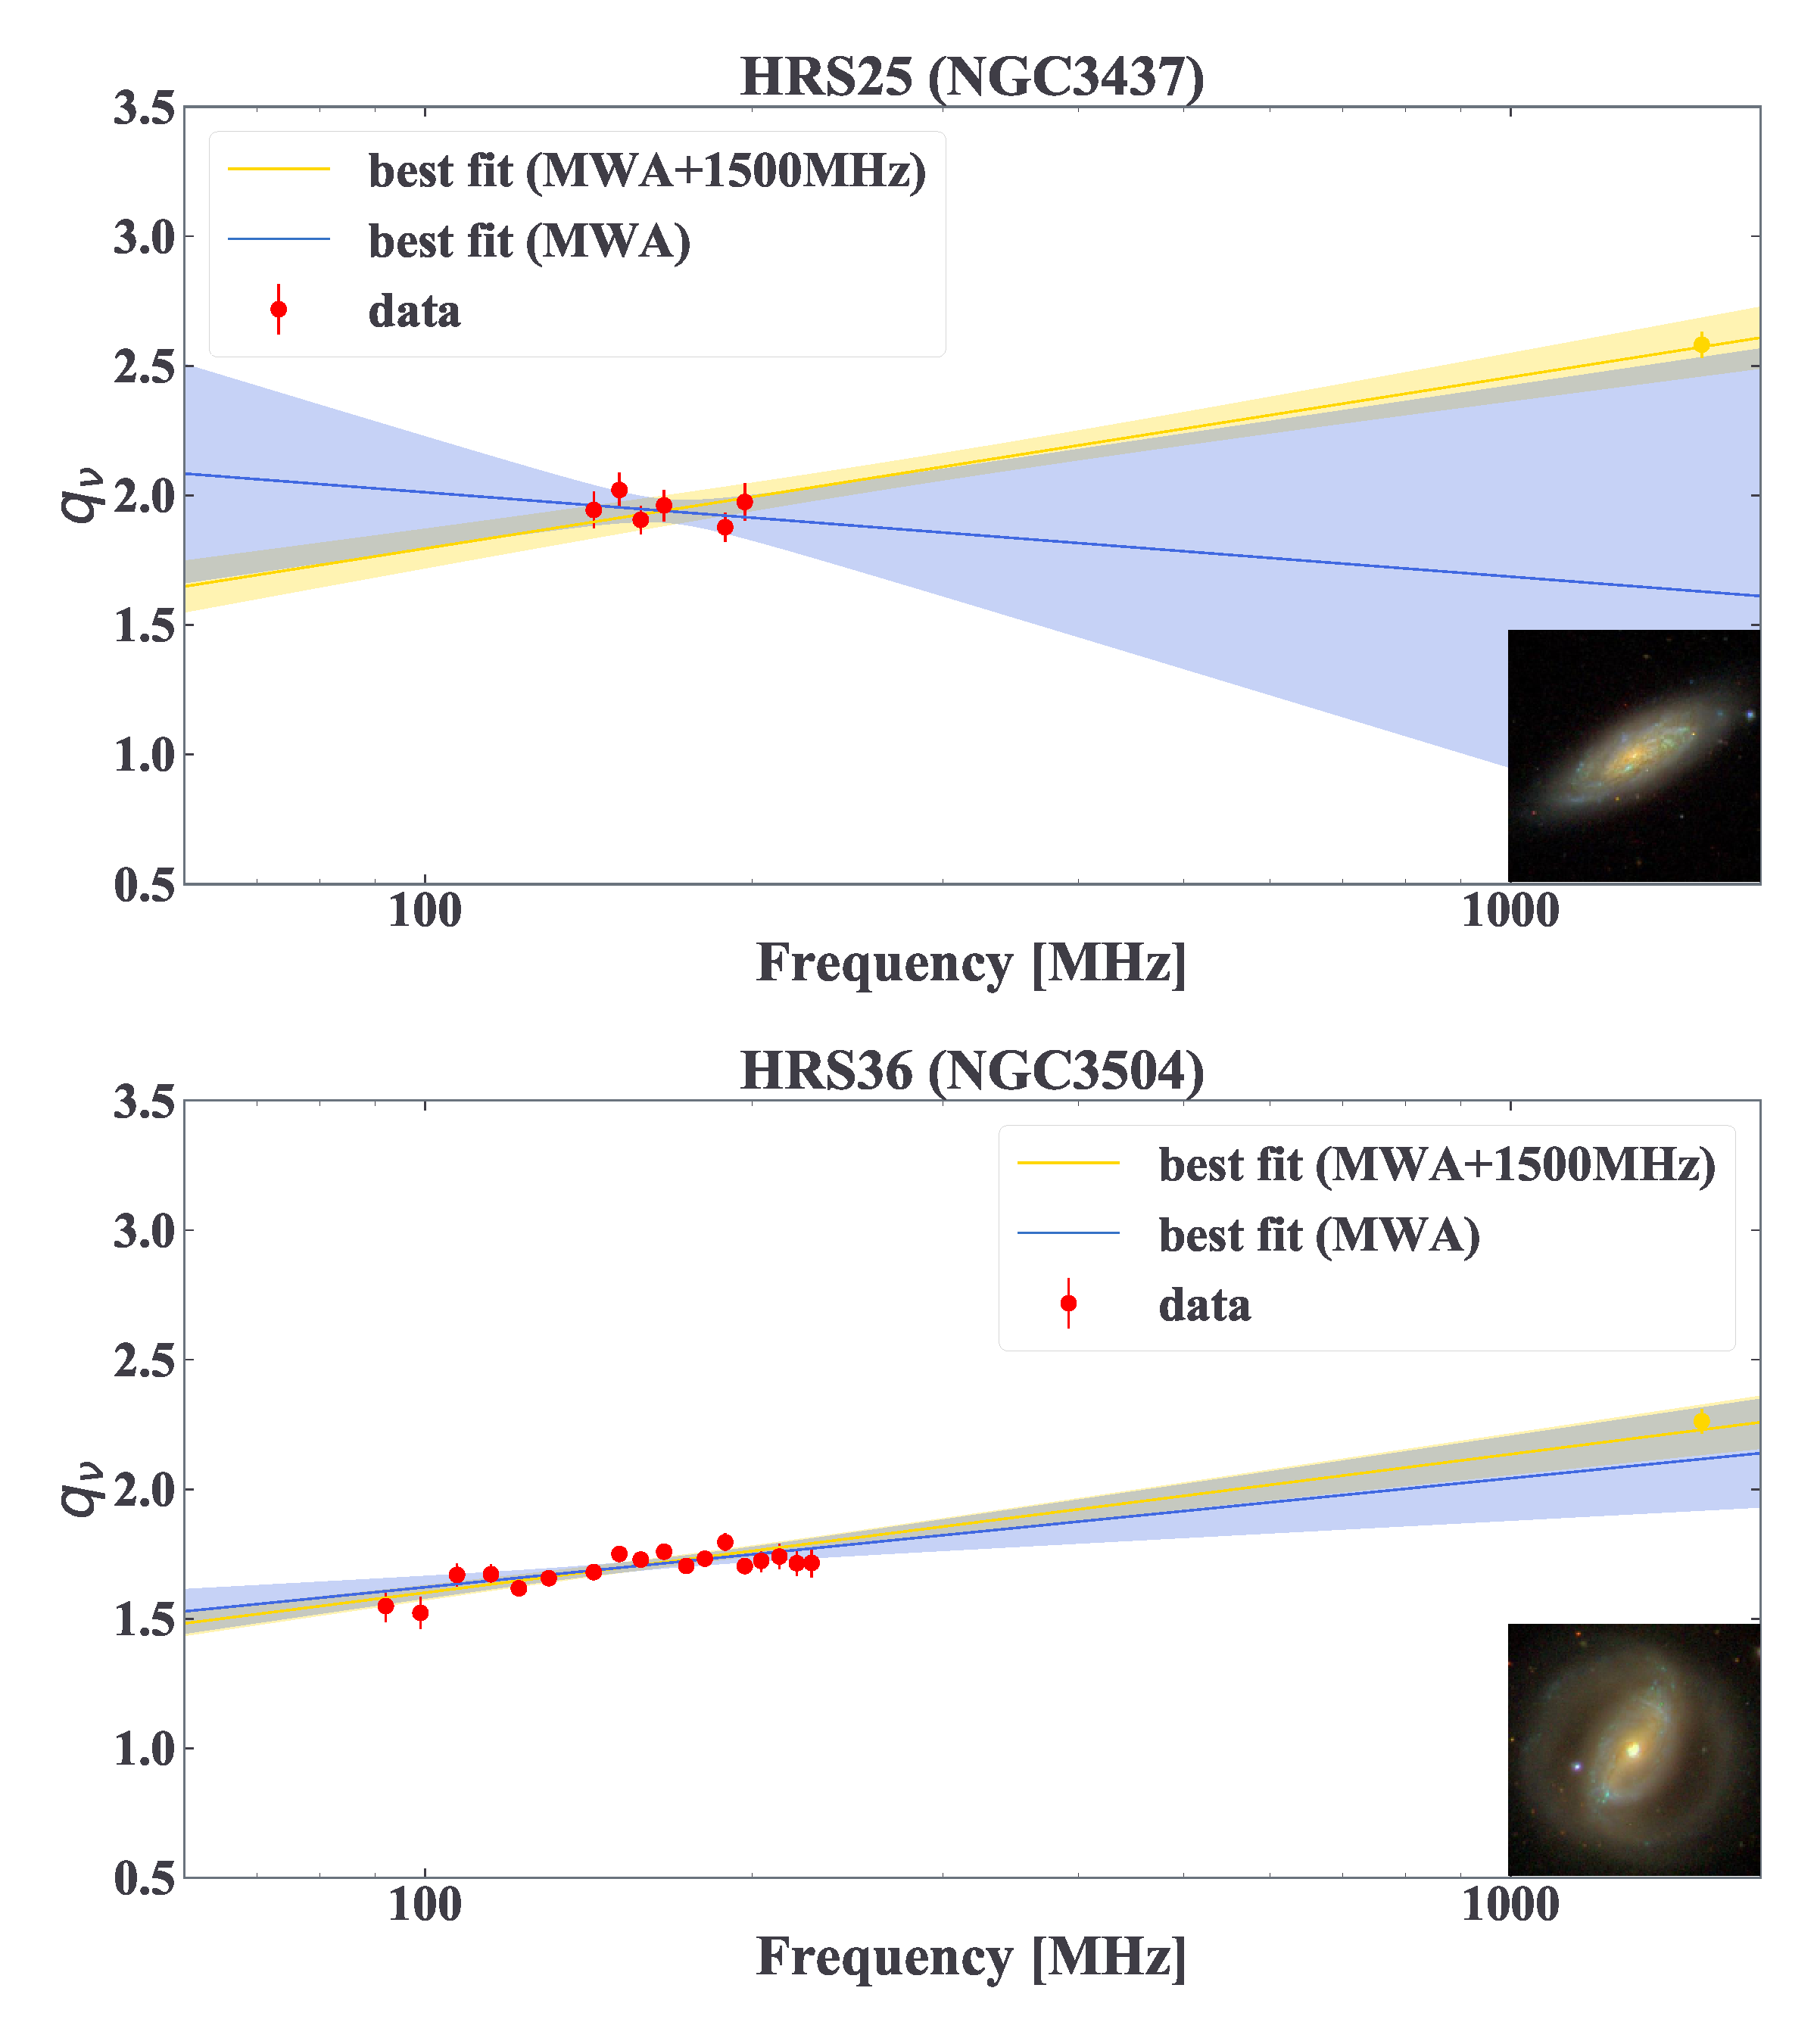
\includegraphics[width=.85\linewidth]{Figures/AppendixC_qfitting1.pdf}
    \caption[Fitting results for 18 samples (1)]{\label{fig:fittingresults1}
        These figures show the fitting result.
        Red points show fluxes at each MWA frequency, and a yellow point shows the flux at $1500\MHz$ \citep{Boselli2015}.
        Blue solid line shows the best fitting line, and the shaded region represents the 95\% confidence interval for the fitting to MWA frequencies.
        Yellow line and shaded area show the fitting result with $1500\MHz$ besides MWA frequencies (For HRS122, 163 and 204, we do not display these because of the lack of high-quality data at $1500\MHz$ data).
        On the bottom right, we show the SDSS-RGB stacking image for each galaxy.
    }
\end{figure}

\begin{figure}[htbp]
    \centering
    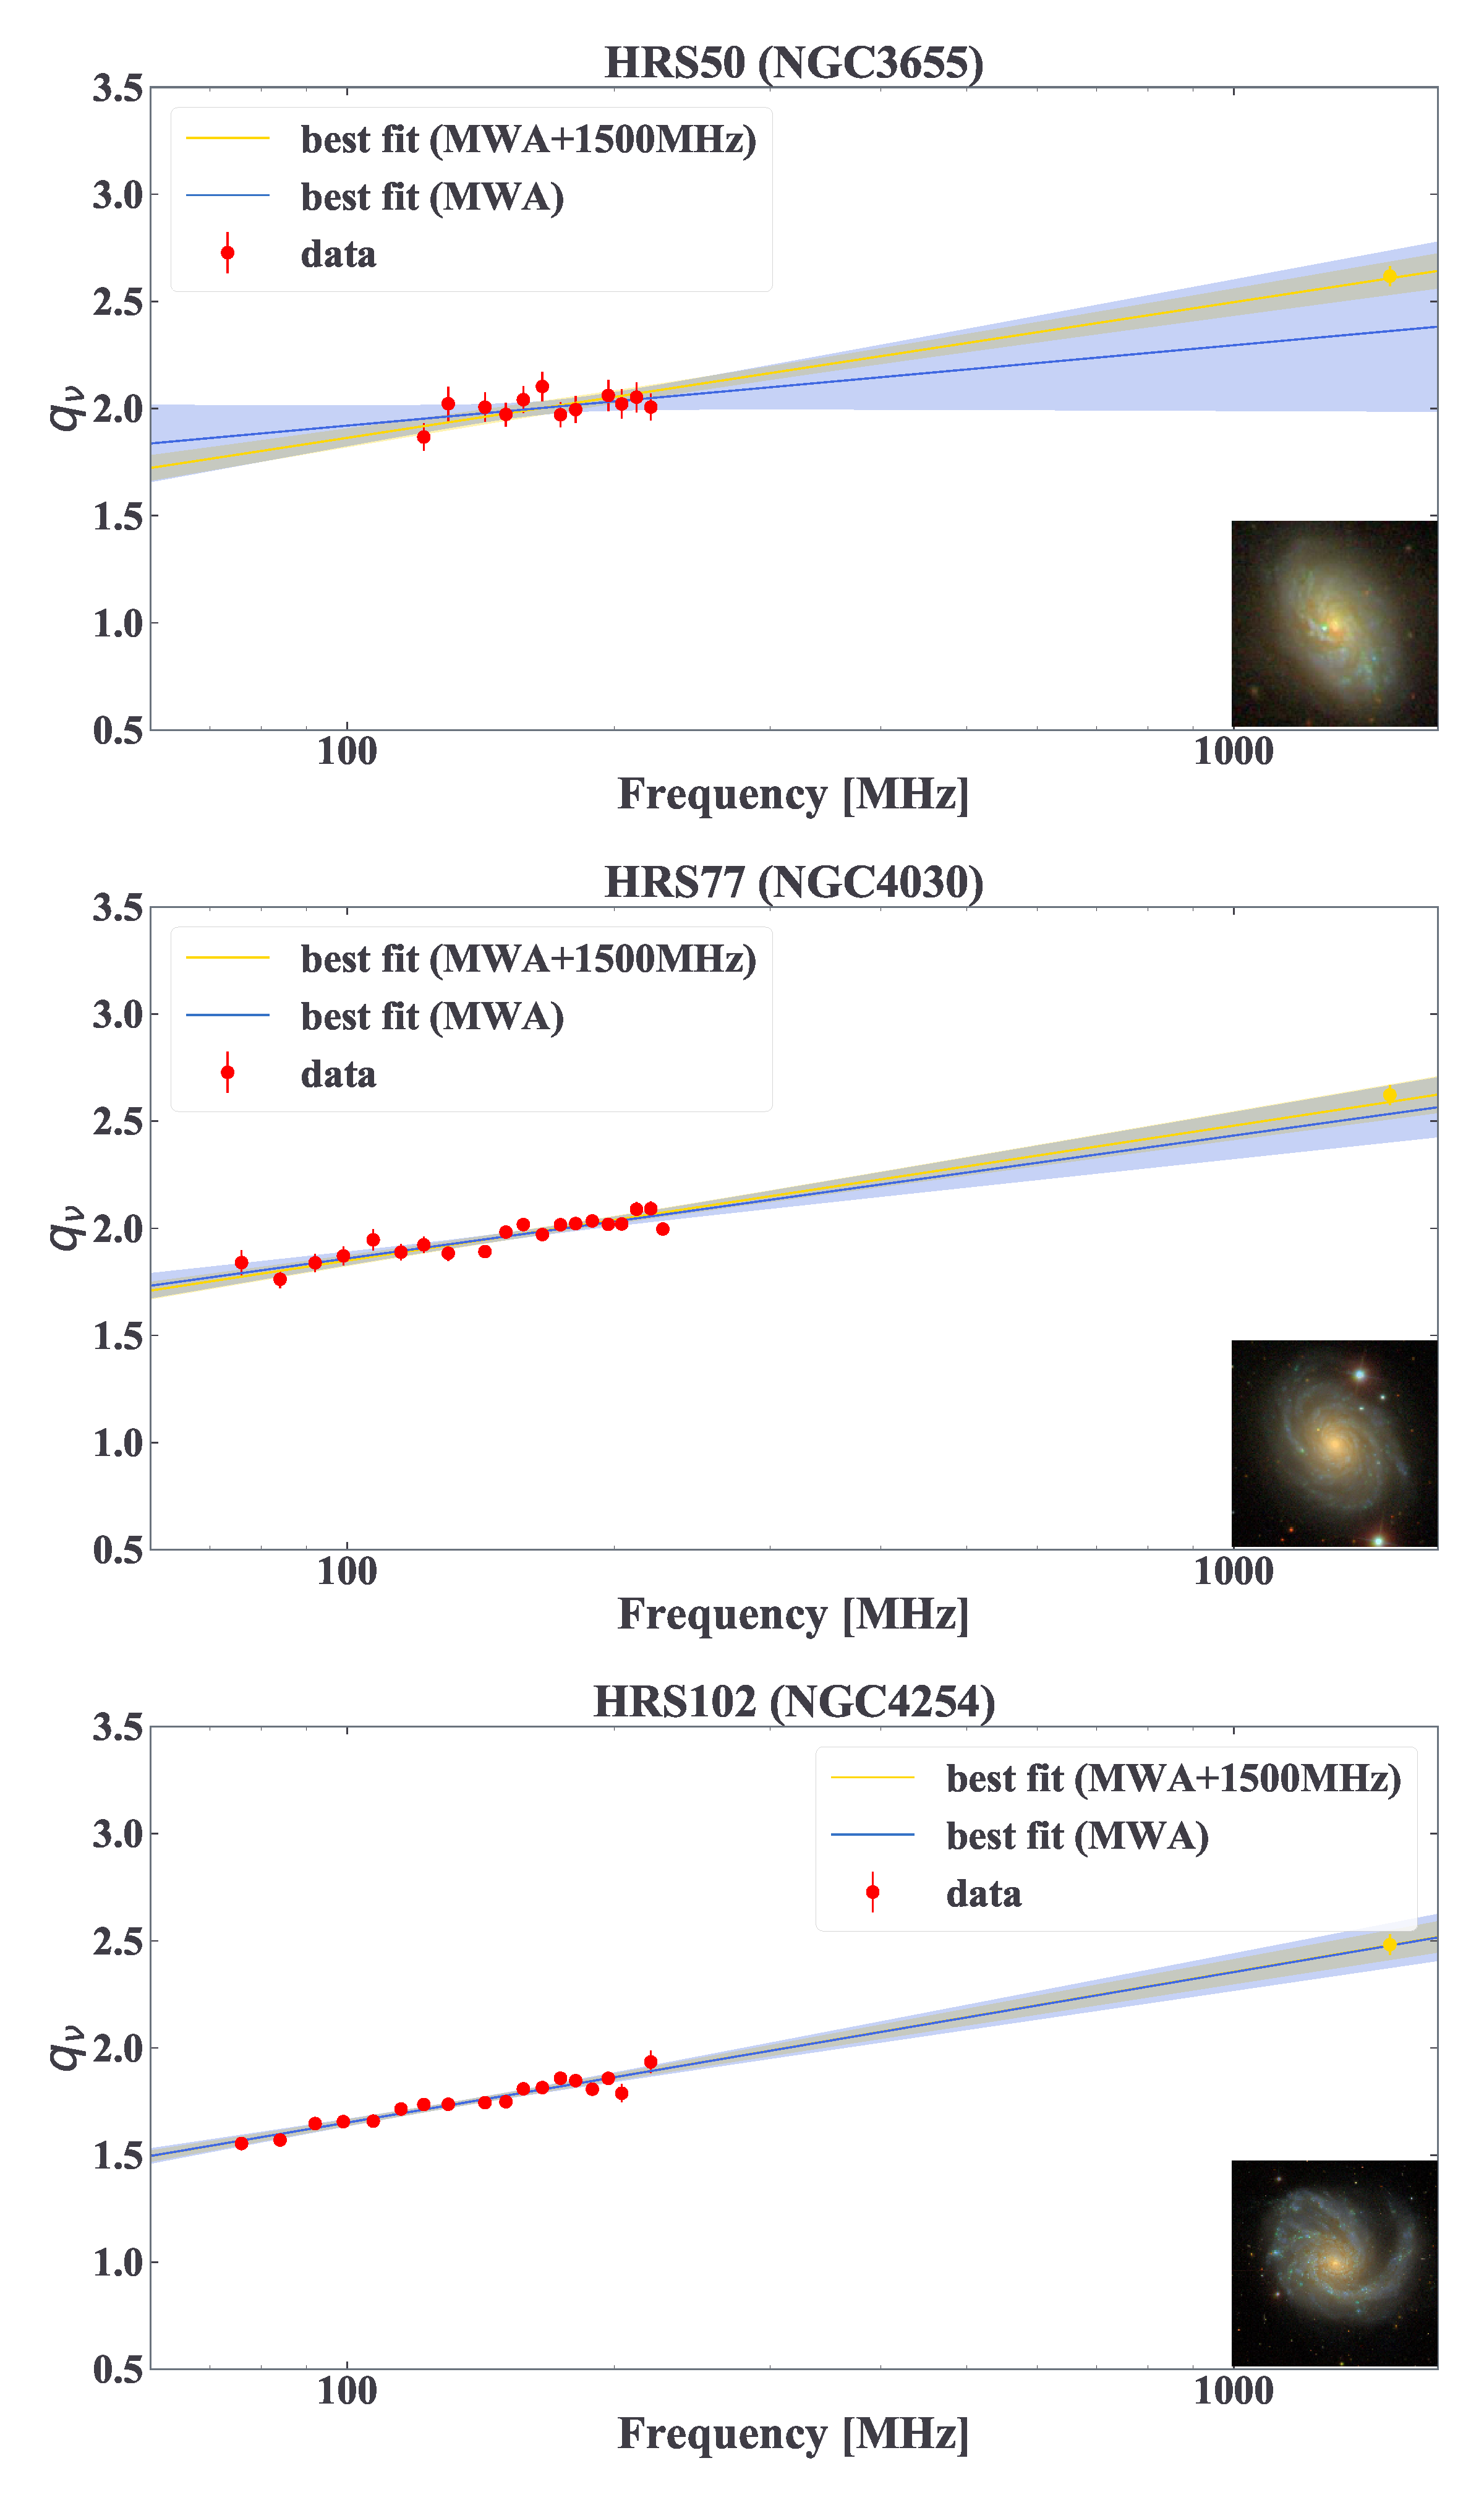
\includegraphics[width=.85\linewidth]{Figures/AppendixC_qfitting2.pdf}
    \caption[Fitting results for 18 samples (2)]{\label{fig:fittingresults2}
        Continuous.
    }
\end{figure}

\begin{figure}[htbp]
    \centering
    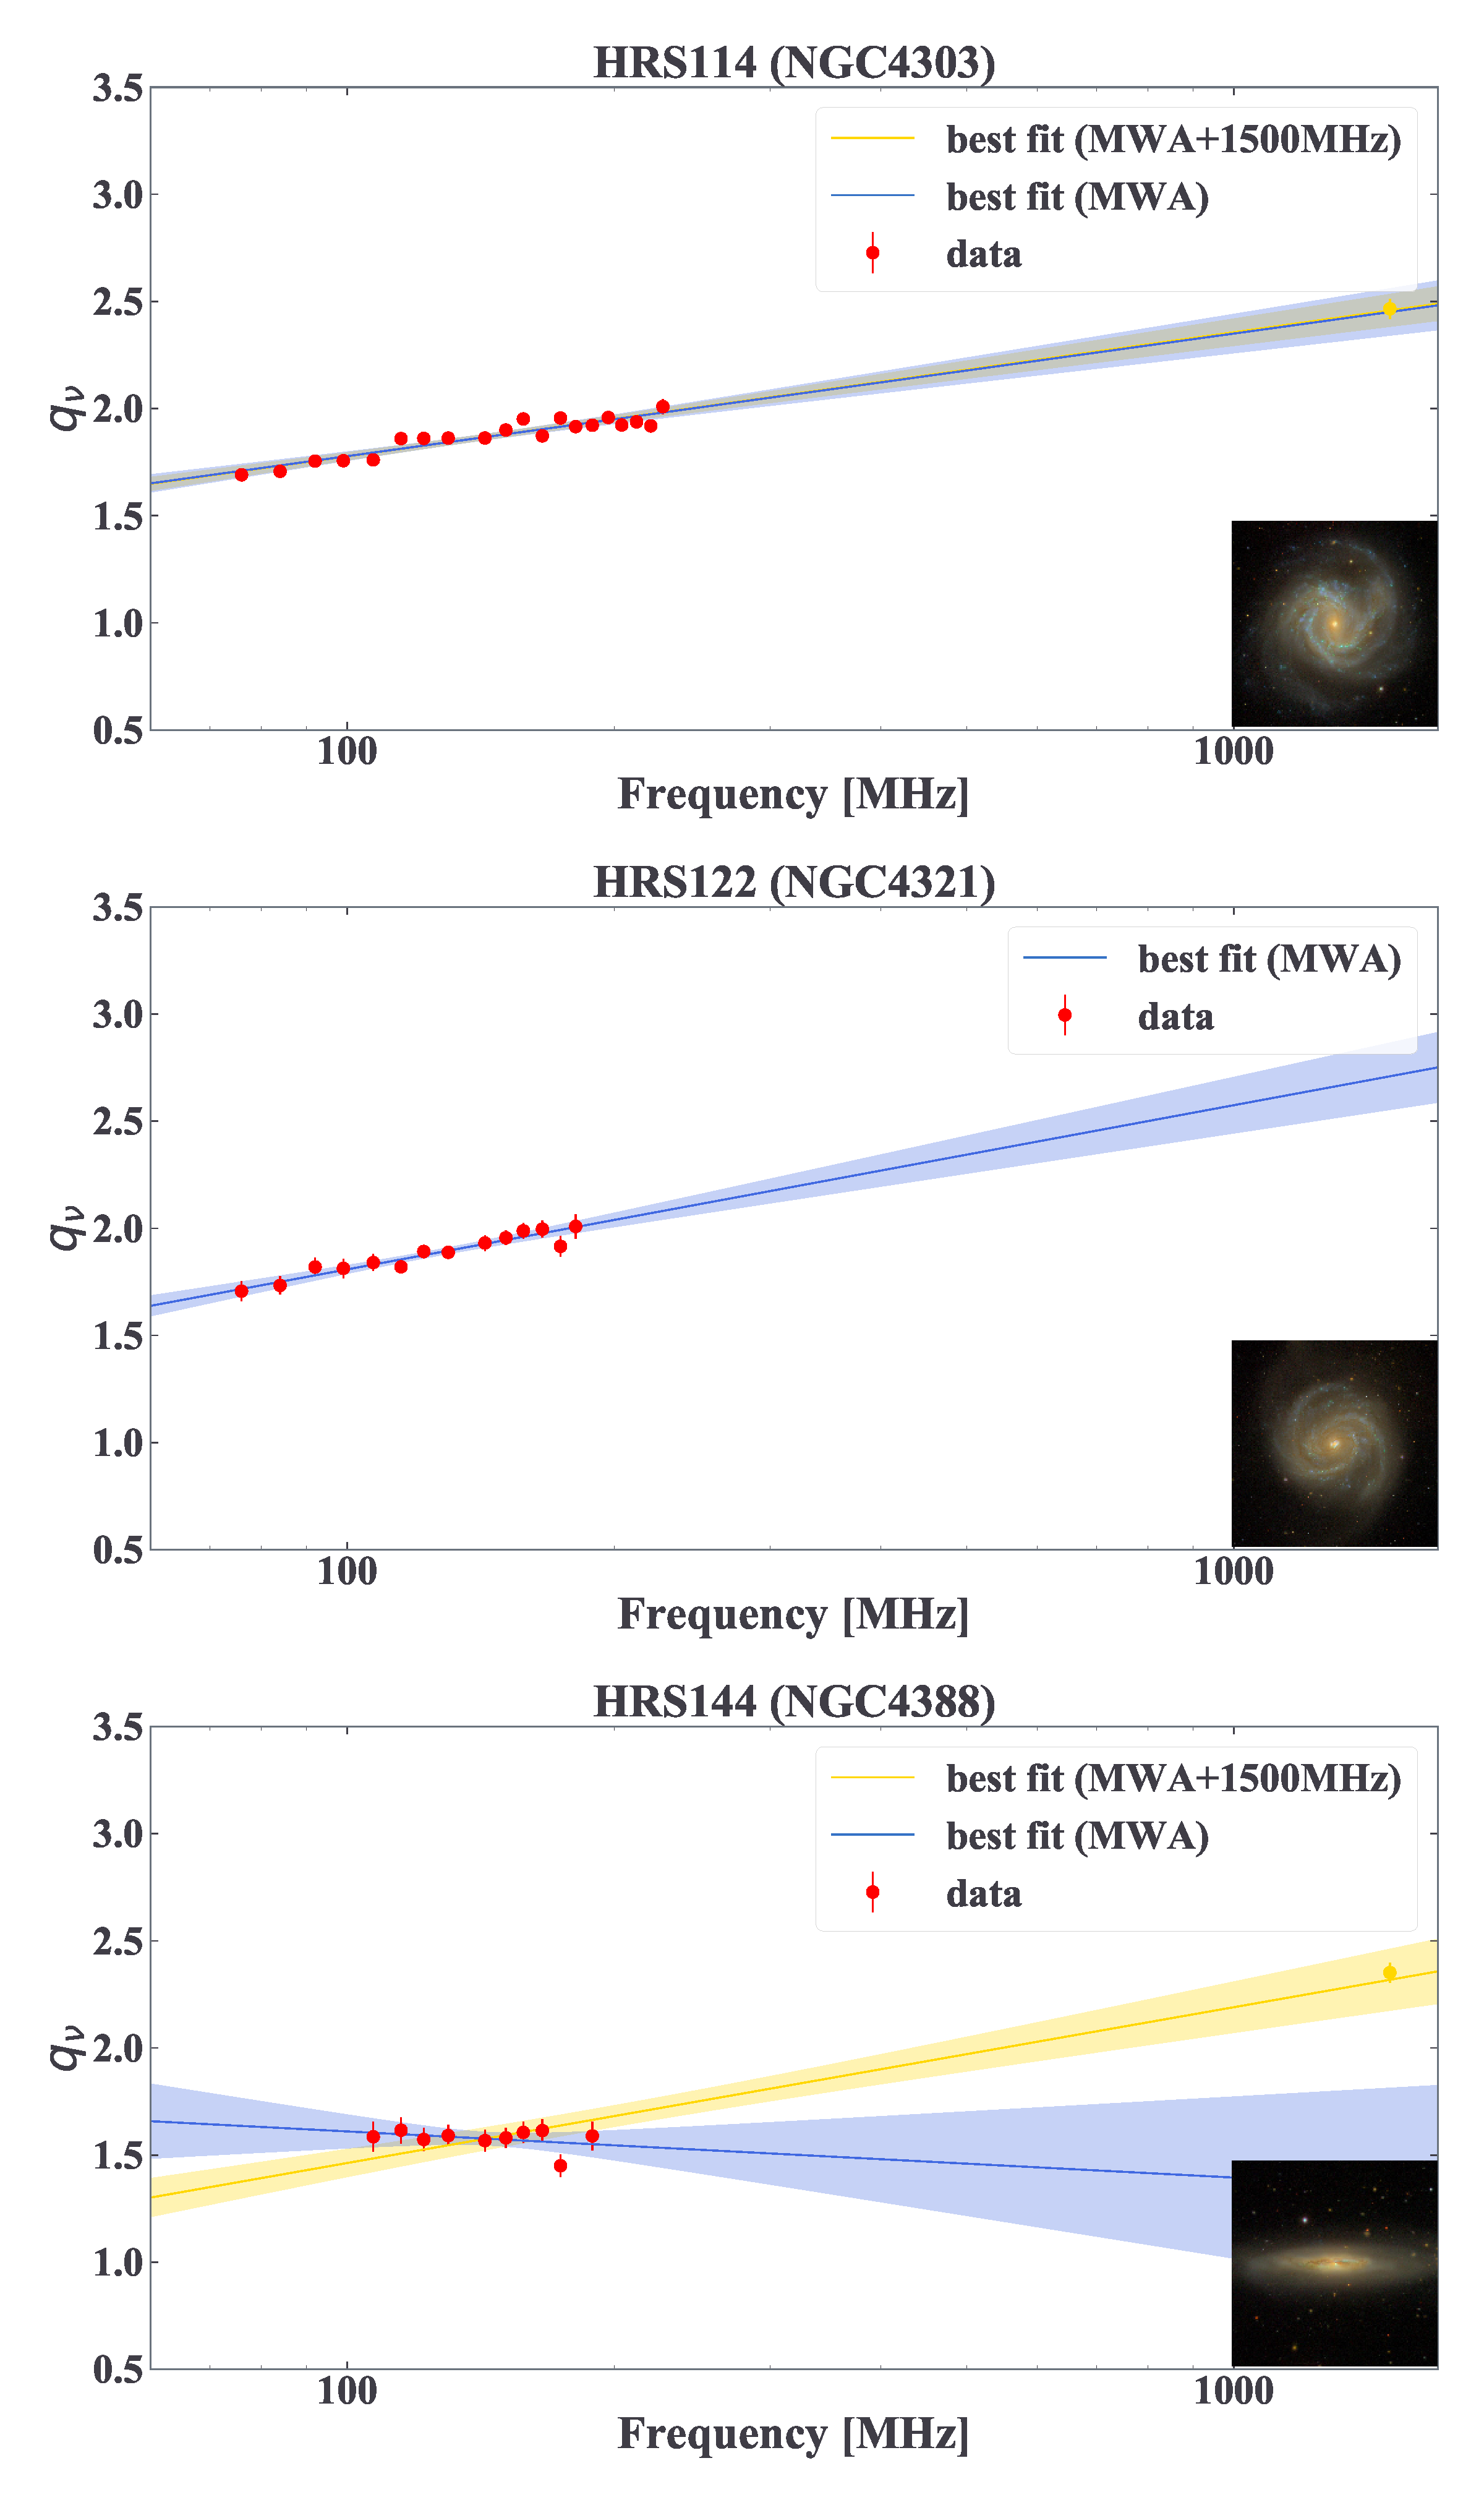
\includegraphics[width=.85\linewidth]{Figures/AppendixC_qfitting3.pdf}
    \caption[Fitting results for 18 samples (3)]{\label{fig:fittingresults3}
        Continuous.
    }
\end{figure}

\begin{figure}[htbp]
    \centering
    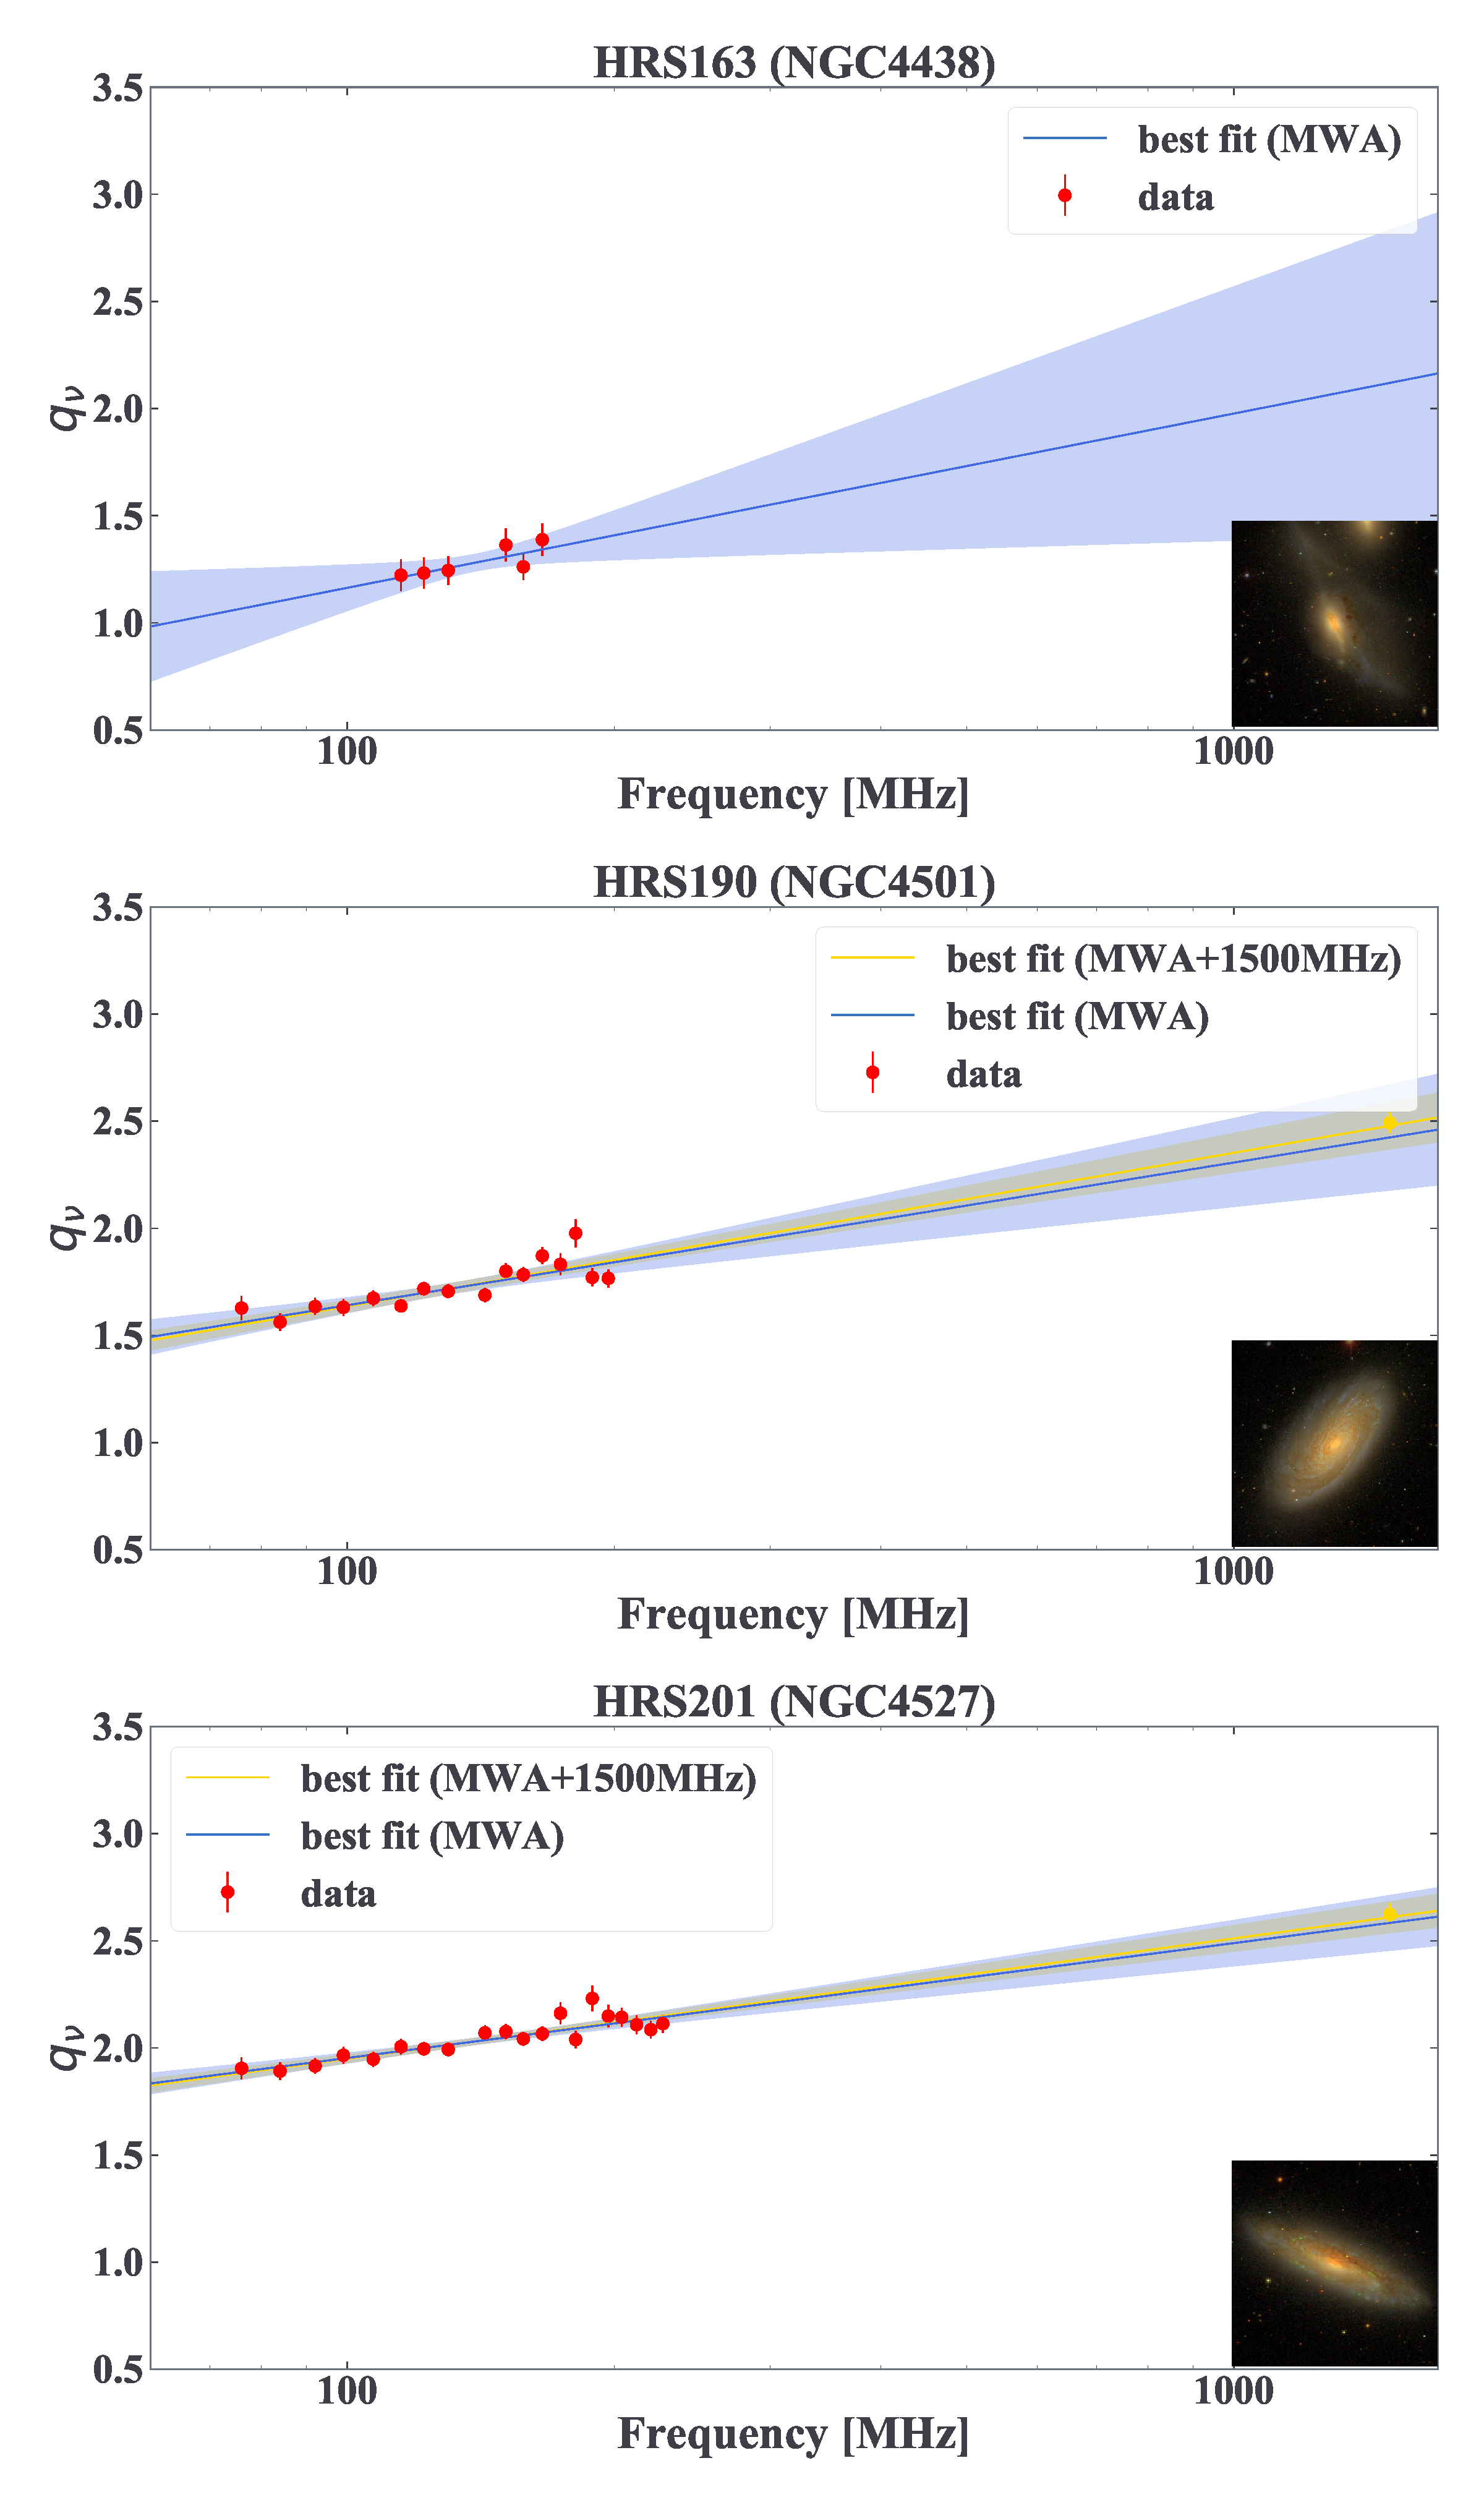
\includegraphics[width=.85\linewidth]{Figures/AppendixC_qfitting4.pdf}
    \caption[Fitting results for 18 samples (4)]{\label{fig:fittingresults4}
        Continuous.
    }
\end{figure}

\begin{figure}[htbp]
    \centering
    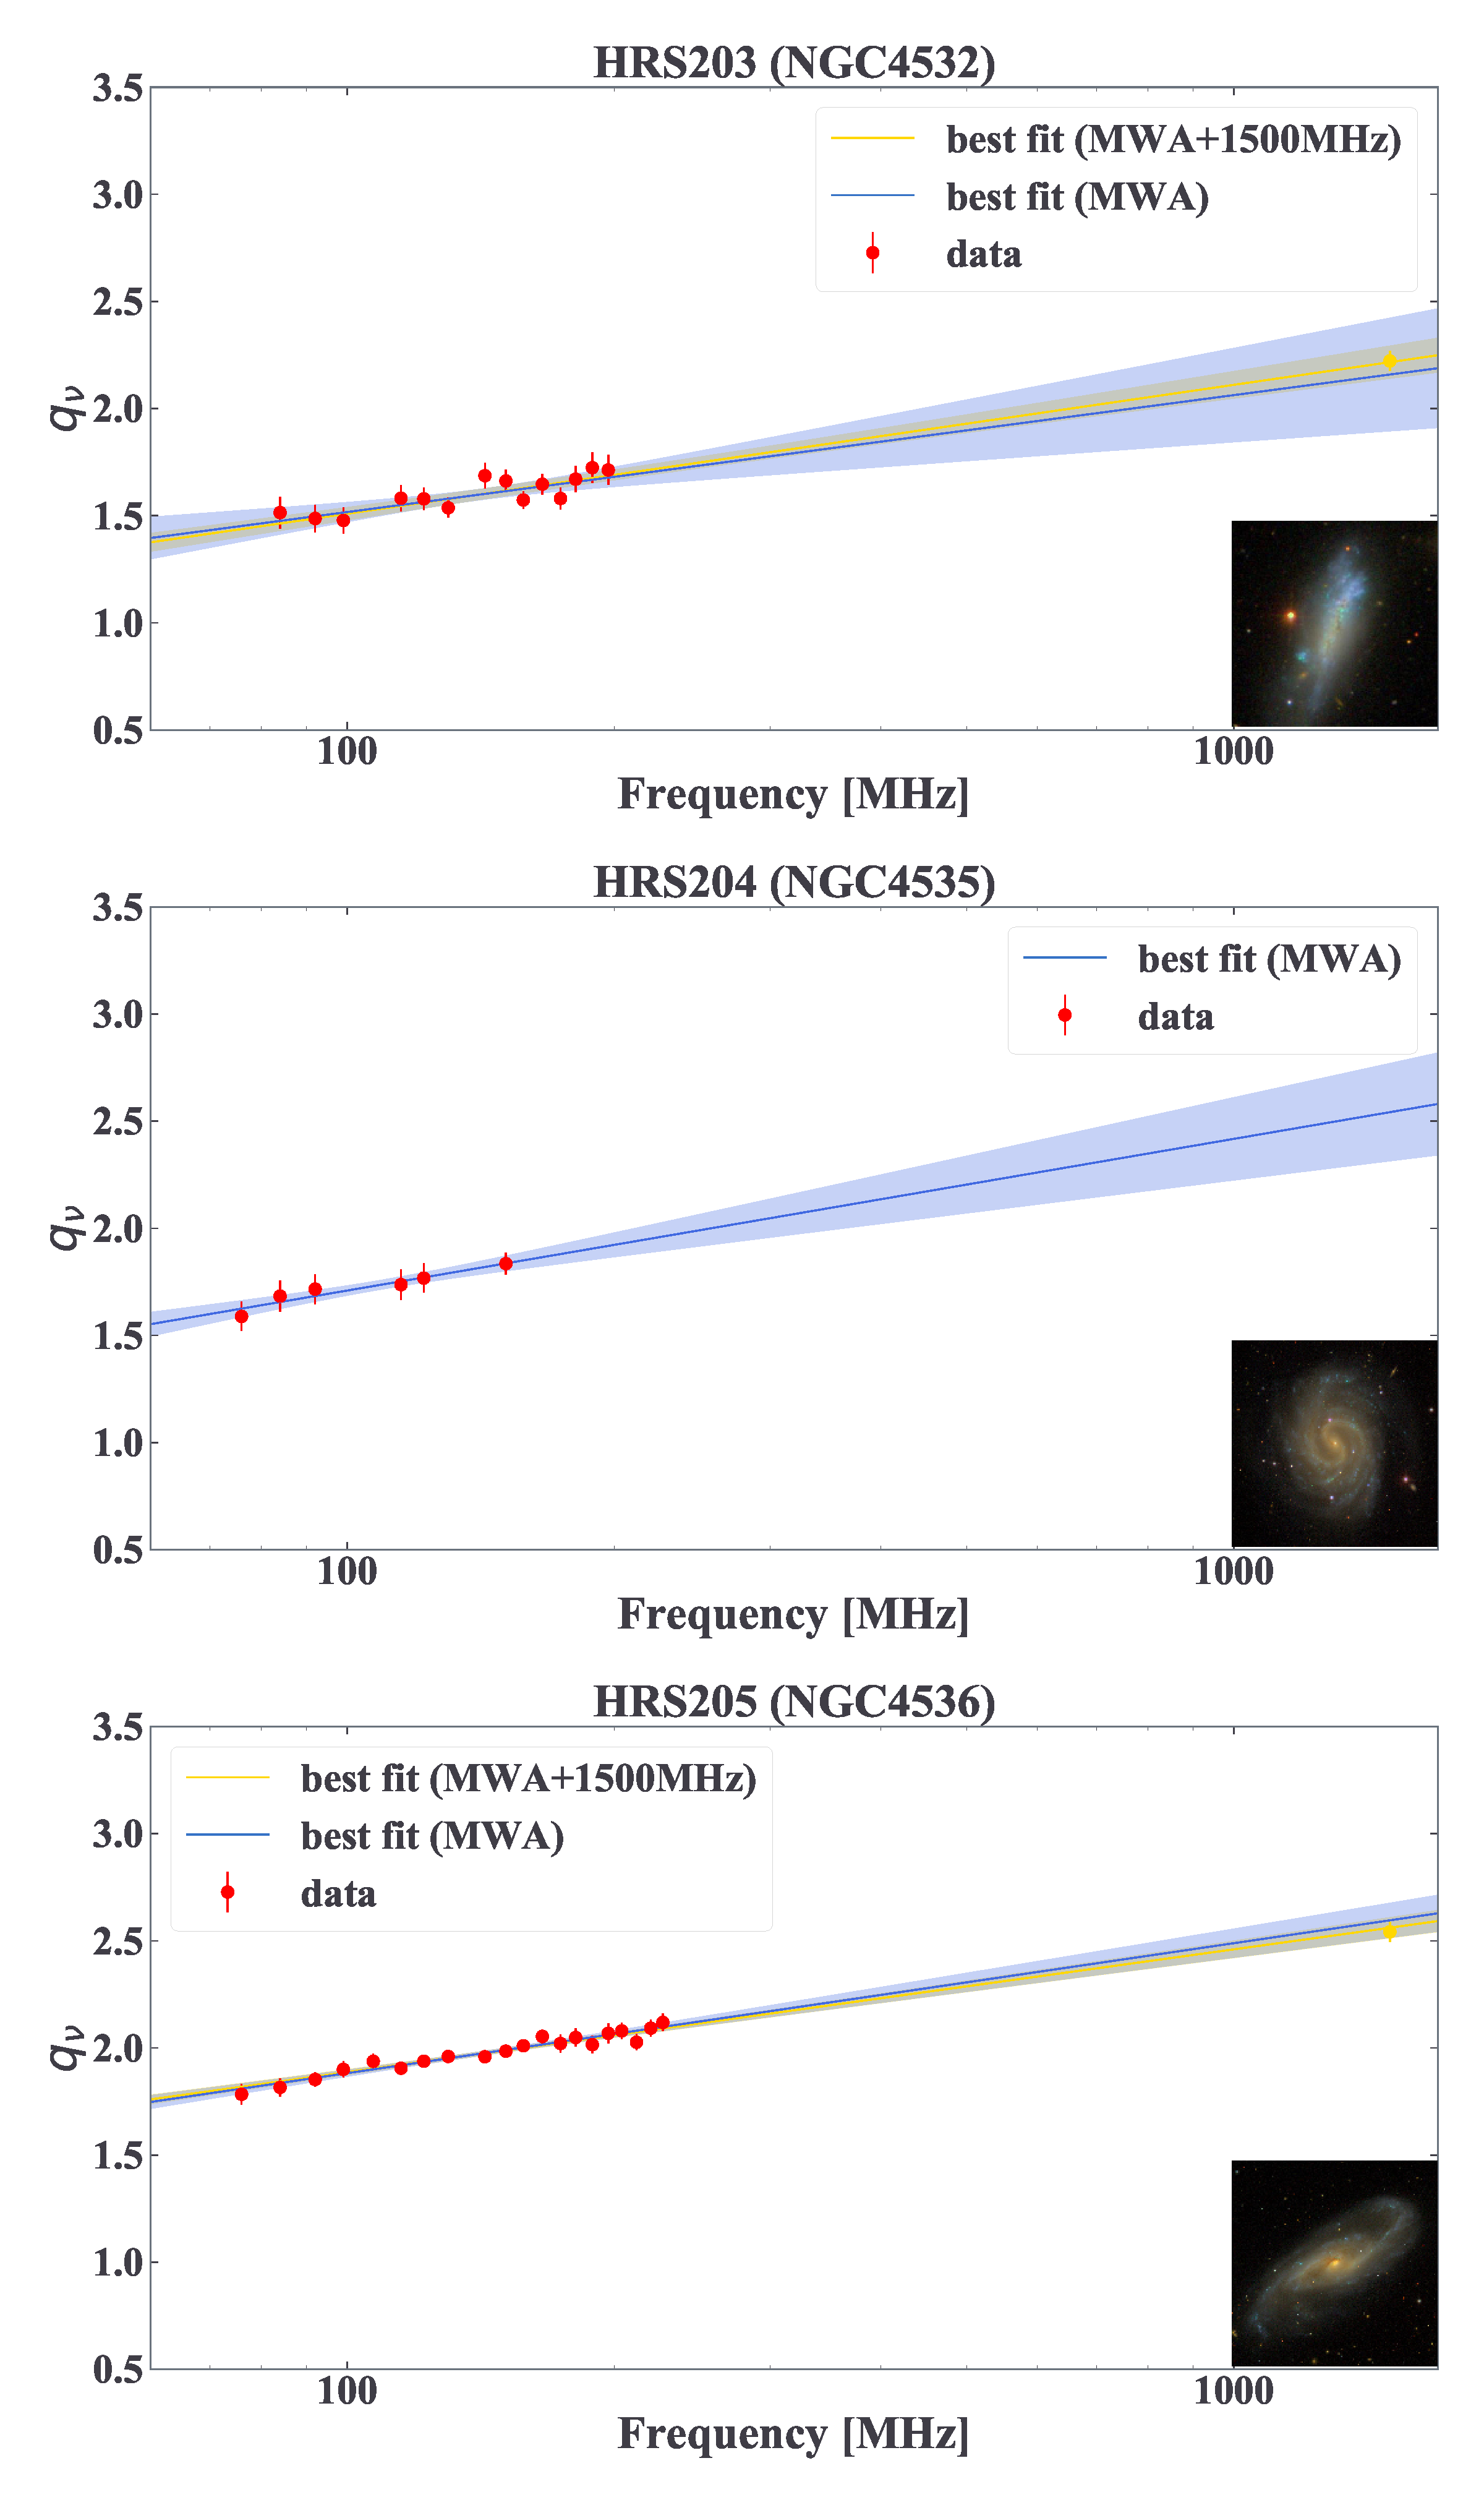
\includegraphics[width=.85\linewidth]{Figures/AppendixC_qfitting5.pdf}
    \caption[Fitting results for 18 samples (5)]{\label{fig:fittingresults5}
        Continuous.
    }
\end{figure}

\begin{figure}[htbp]
    \centering
    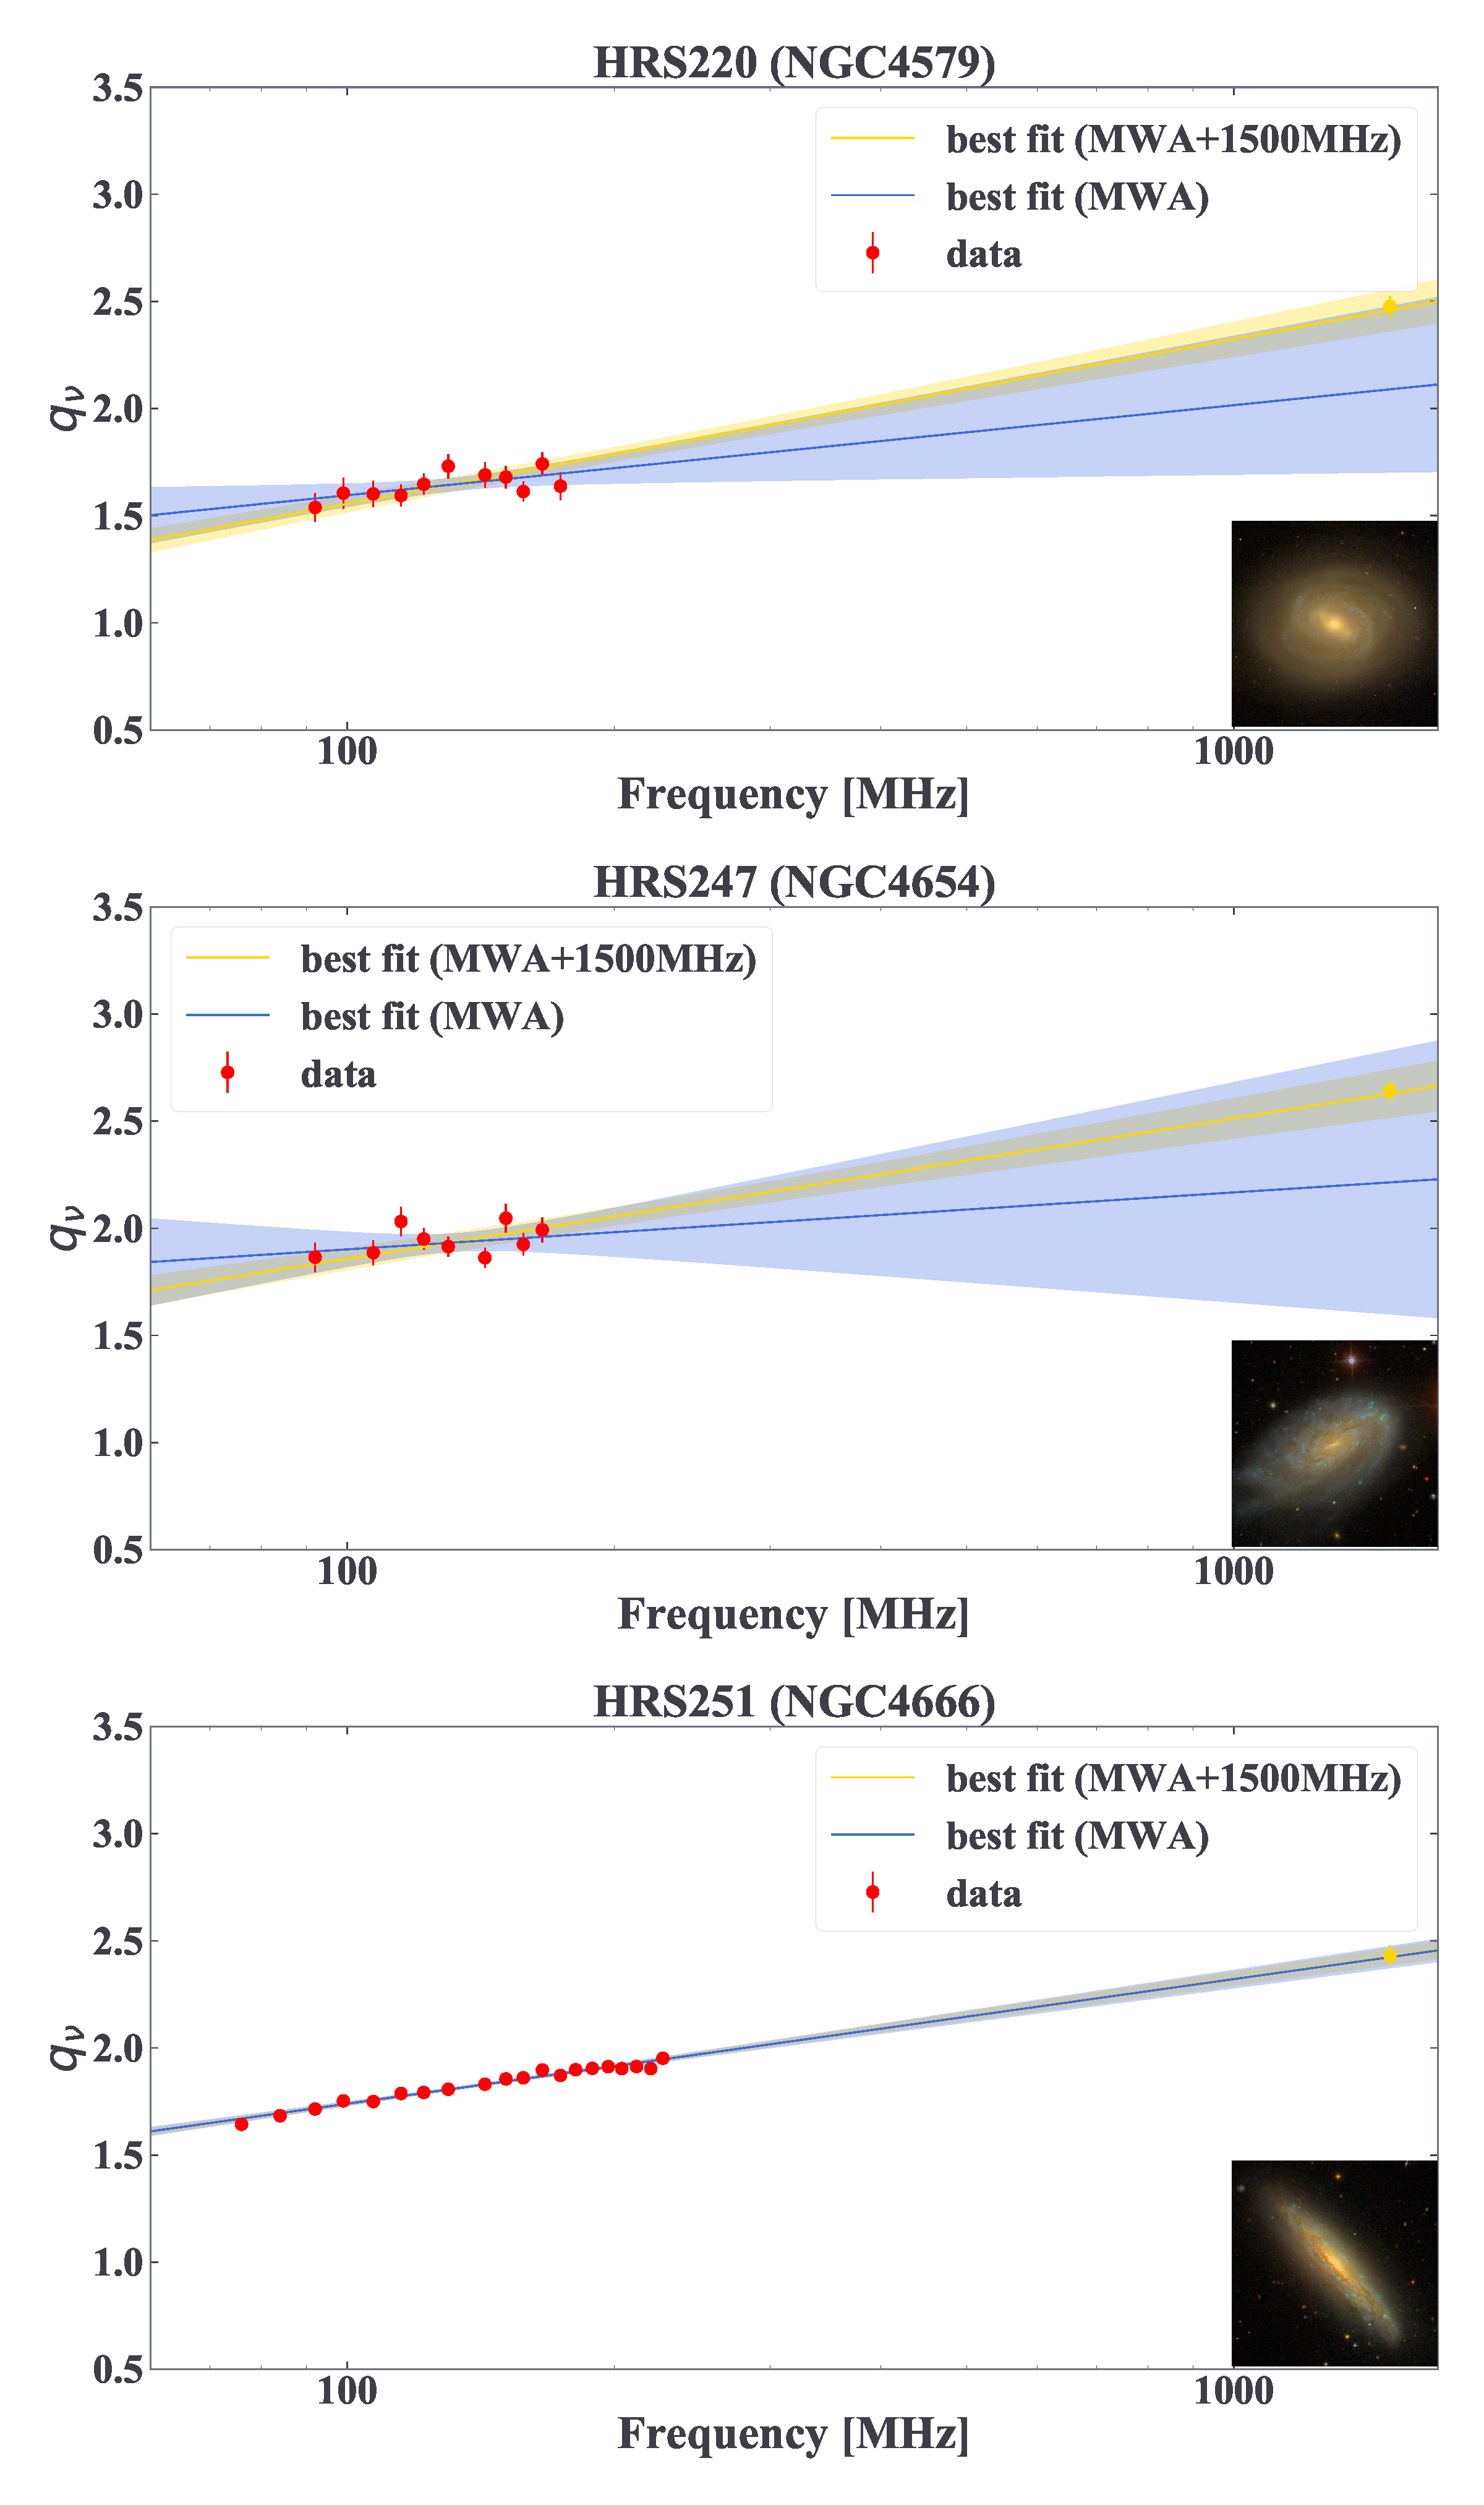
\includegraphics[width=.85\linewidth]{Figures/AppendixC_qfitting6.pdf}
    \caption[Fitting results for 18 samples (6)]{\label{fig:fittingresults6}
        Continuous.
    }
\end{figure}

\begin{figure}[htbp]
    \centering
    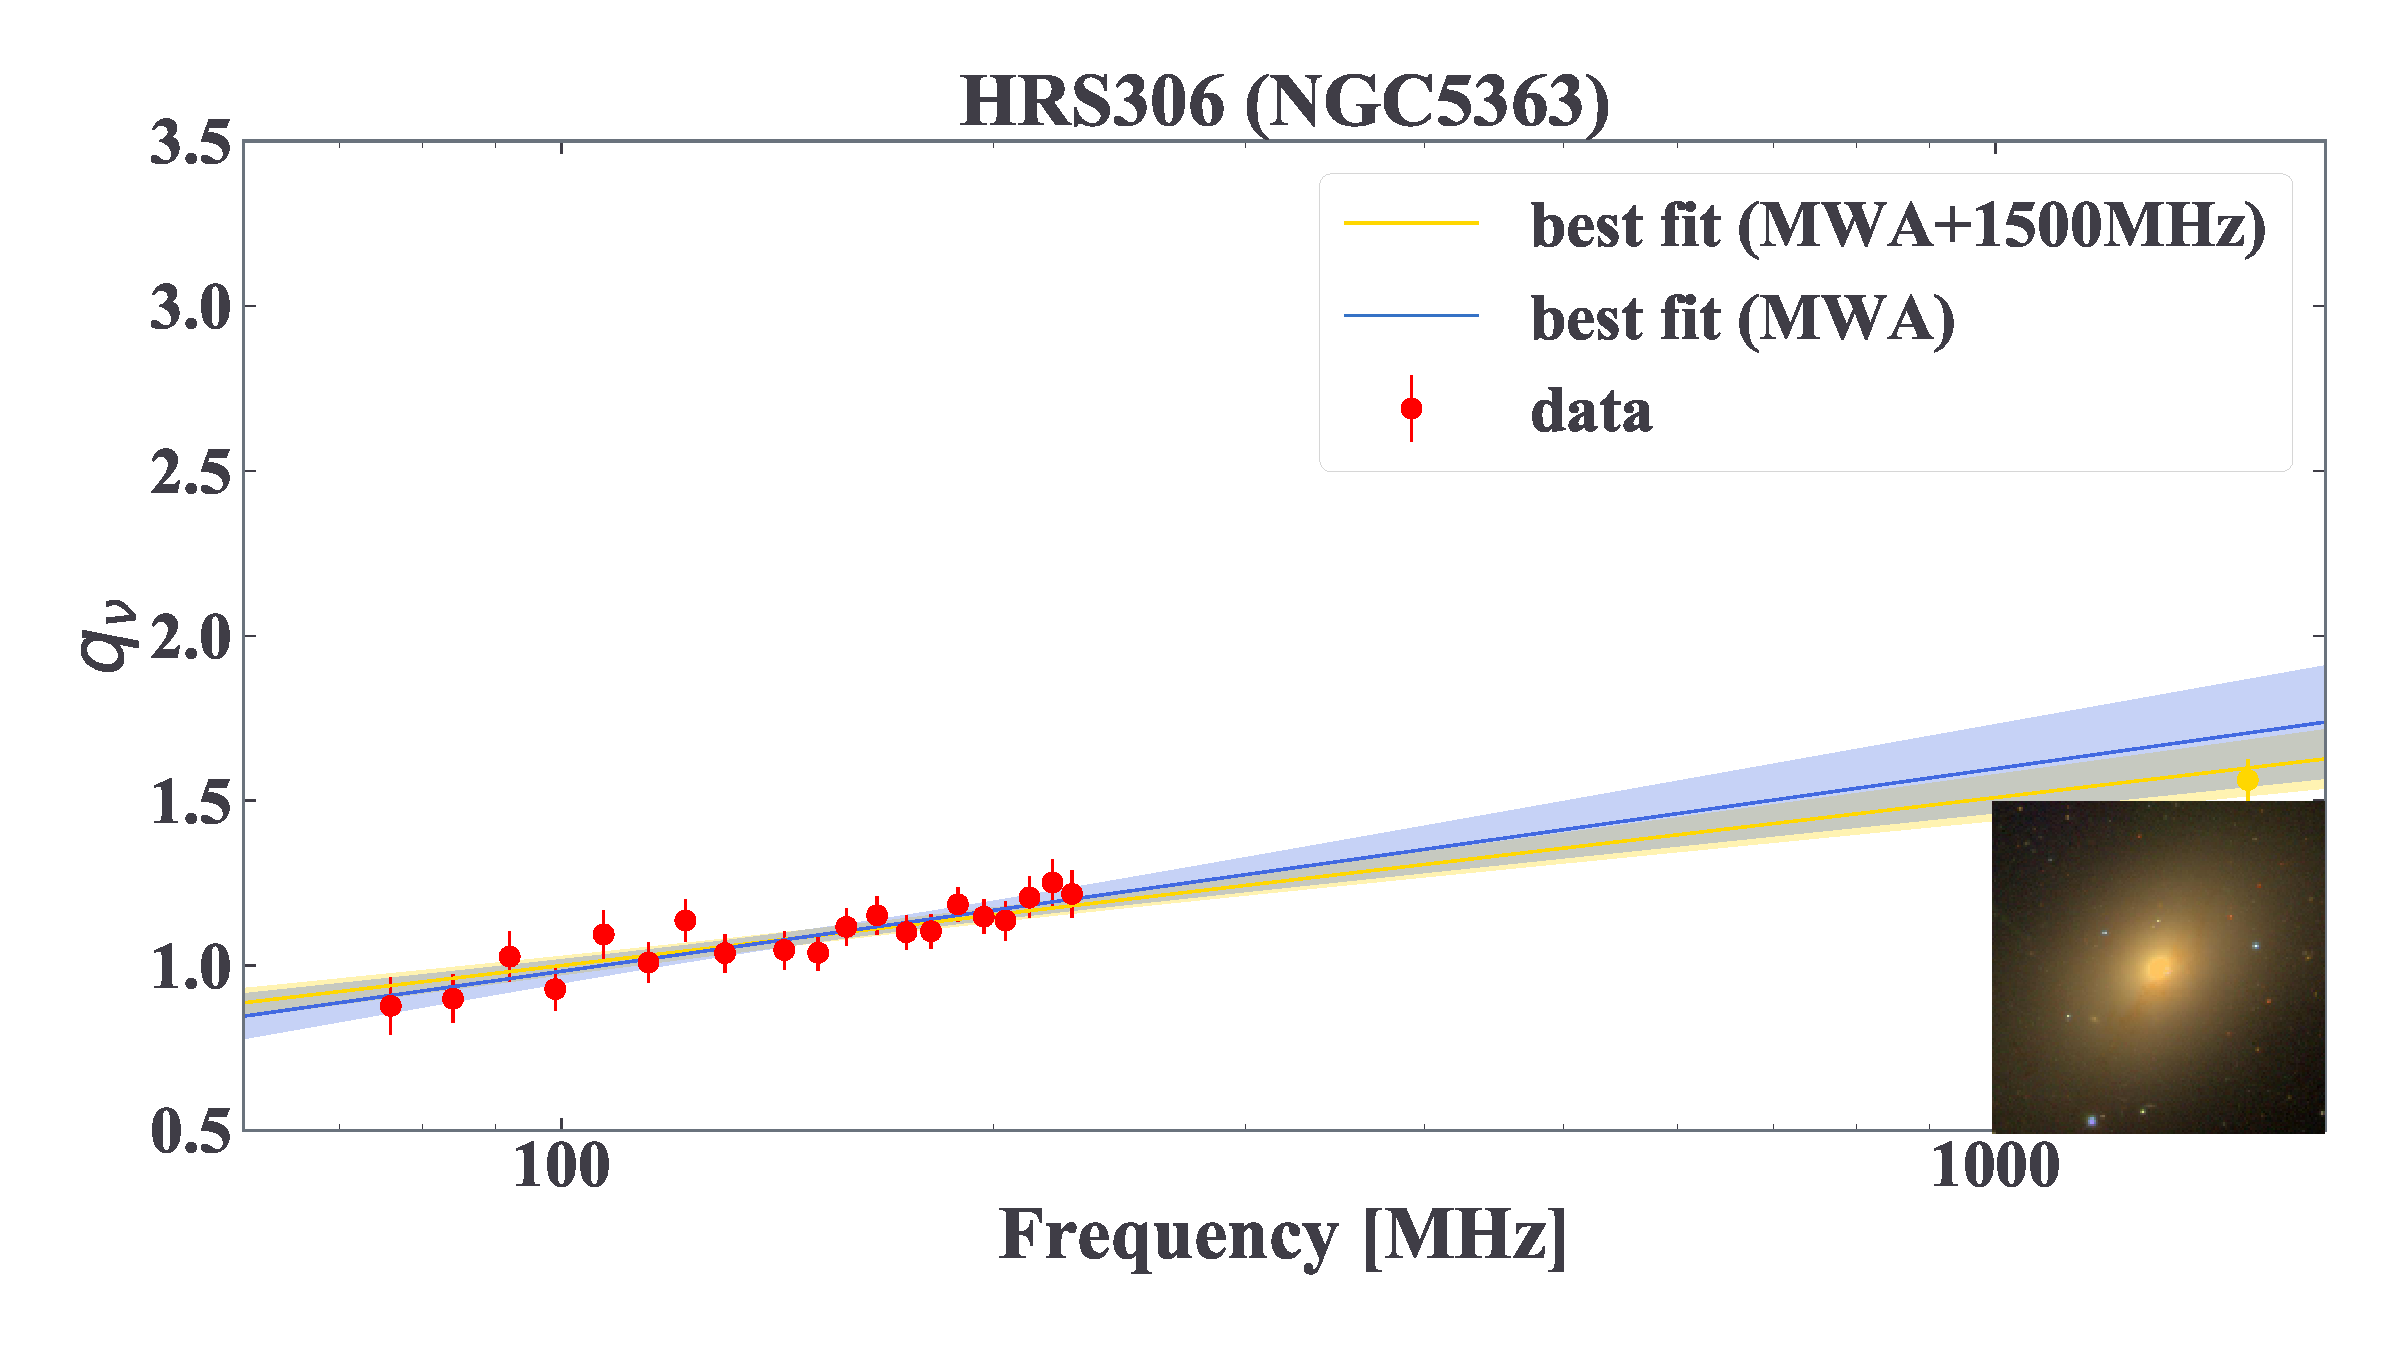
\includegraphics[width=.85\linewidth]{Figures/AppendixC_qfitting7.pdf}
    \caption[Fitting results for 18 samples (7)]{\label{fig:fittingresults7}
        Continuous.
    }
\end{figure}

\end{document}
